\chapter{Application: Cardiac Mechanics}
\label{chap:5}
%
Provided the image-based meshing workflow fully developed in~\chapref{3}, together with the finite element approaches established in~\chapref{4}, the entire image-based modeling and simulation pipeline is demonstrated through modeling the mechanical behavior of a beating human heart. Cardiac mechanics is a good testbed for the particular image-based modeling and simulation workflow described because: 1) the application only involves binary image masks, 2) the exact geometry does not grossly affect results since contact modeling is not included, and 3) the use of simulation in this field arguably has the potential to save and improve more lives than any other biomechanics application area.

This chapter introduces and motivates the task of modeling the human heart. The essential components to computational cardiac mechanics are described for an implementation using conventional finite elements, and  simulation results are presented. Finally, the details of implementing the same mechanics into the polyhedral code \textit{Celeris} are discussed, along with verification results.

\section{Introduction}

A brief overview of the anatomy and function of the heart will be presented, followed by a survey of approaches found in the literature.

\subsection{Anatomy and Function of the Heart}
The heart consists of four chambers: the \textit{left ventricle} (LV), \textit{right ventricle} (RV), \textit{left atria} (LA), and \textit{right atria} (RA) (See~\figref{anatomy}). The \textit{septum} is the tissue wall that separates the LV and RV. The thinner-walled atria act as blood reservoirs for the ventricles, which are predominantly responsible for the pumping function. The entire heart is encompassed by a fibrous sac known as the \textit{pericardium}, which resists rapid increases in cardiac size. The primary function of the heart is to pump blood throughout the body, delivering nutrients and removing waste from each organ~\cite{holzapfel_2009}. Cyclic pumping of the heart arises from the interaction of its electrical and mechanical function. Namely, the electrical activation of cardiac muscle fibers causes an excitation and contraction of tissue that drives the motion of the organ. Myocardial tissue consists of discrete muscle fiber bundles that exhibit orthotropic material behavior. For a more detailed description of the macro and microstructural properties of the heart, refer to Holzapfel \textit{et al.}~\cite{holzapfel_2009} and Hunter~\cite{holzapfel_2009} 

\begin{figure}[htbp!]
\centering
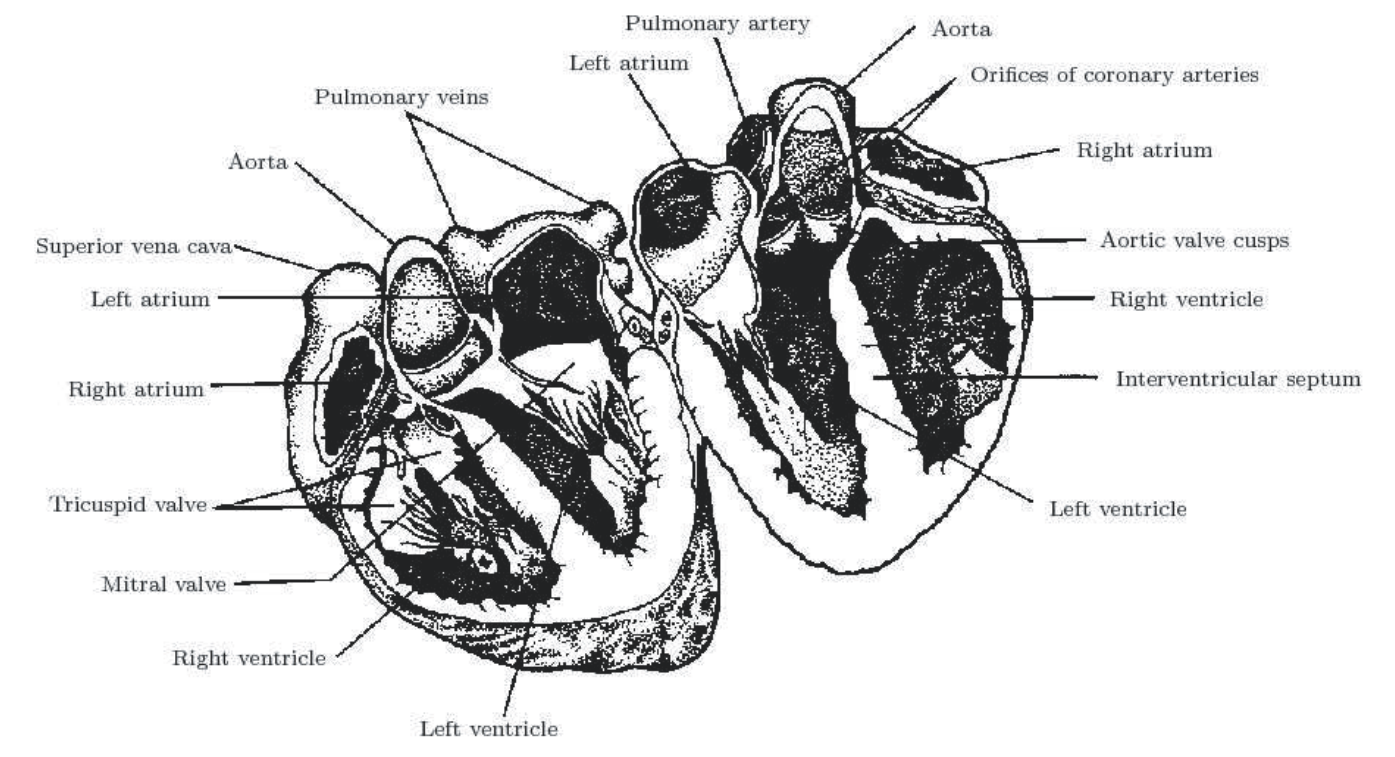
\includegraphics[width=1.0\textwidth]{media/anatomy.png}
\caption{Longitudinal cross-section of the human heart~\cite{katz_2015}}
\label{fig:anatomy}
\end{figure}

\subsection{Related Work}
Cardiovascular disease is the leading cause of death and disability, accounting for about 40$\%$ of all human mortality~\cite{genet_2015}. Heart failure is one of the most common, costly, and deadly medical conditions, affecting more than 25 million people worldwide~\cite{mann_2015}. Better understanding the nuanced electrical and mechanical behavior of normal and pathological hearts is an important step in improving treatment for heart disease. The complexity of the mechanisms of interest, time and cost savings offered by simulation, and the high sensitivity to various patient-specific parameters make \textit{in silico} modeling an important tool in addressing heart disease.

Indeed, cardiac mechanics is one of the most mature fields in computational biomechanics. Several well-known groups have advanced the field using a variety of approaches with respect to the geometry and meshing. \textit{The Living Heart Project}~\cite{genet_2015, baillargeon_2014} has arguably gained the most traction in advancing the understanding of whole-heart cardiac mechanics through simulation, albeit using linear tetrahedra for an artificial heart geometry not generated from medical imaging. Augustin \textit{et al.}~\cite{augustin_2016} also used linear tetrahedral finite elements, meshed from considerably smoothed surfaces originating from MRI data. Pleny of informative research still only models simplified geometries of the left ventricle~\cite{guccione_2005, sack_2016}, in conjunction even with cubic Hermite finite elements~\cite{mcculloch_2000}. Generally speaking, though, most modern approaches generate either bi-ventricular models (i.e., left and right ventricles) or whole heart models that include the atria and potentially other geometric structures.

Gurev \textit{et al.}~\cite{gurev_2015} performed mechanical simulations on a quadratic hex-dominant mixed element mesh of the human heart ventricles, whose work forms the basis for the cardiac mechanics explorations detailed in this chapter. The review article by Trayanova \textit{et al.}~\cite{trayanova_2011} provides an excellent summary of the various components involved in ventricular electromechanical modeling, many of which are discussed in this chapter.

\section[Demonstration using Conventional Finite Elements]{Demonstration using Conventional Finite \\ Elements}

The key features of \textit{Cardioid}~\cite{richards_2013, gurev_2015} will be highlighted, as is relevant to image-based cardiac mechanics modeling. Cardioid is a highly efficient and scalable code at Lawrence Livermore National Laboratory that utilizes high performance computing for modeling the electromechanics of cardiac arrhythmia. The code is used here to demonstrate the image-based modeling and simulation pipeline using conventional finite element methods.

%%%%%%%%%%%%%%%%%%%%%%%%%%%%%%%%%%%%%%%%%%%%%%%
%%%%%%%%%%%%%%%%%%%%%%%%%%%%%%%%%%%%%%%%%%%%%%%
\subsection{Methods}
\label{Methods}

In Cardioid, the body is assumed to undergo quasi-static finite deformations, body forces are assumed negligible, and the stress measure of interest is the second Piola-Kirchoff stress $\bm{S}$. Thus, balance of linear momentum reduces to the following equation:
\begin{equation}
(F_{ik}S_{kj}),_{j} = 0
\end{equation}

In order to fully define and solve these equations, the following are specified: the mesh, constitutive update, muscle fiber orientation, solution-dependent pressure boundary conditions, and the finite element solver. Each consideration will be described in turn.

%%%%%%%%%%%%%%%%%%%%%%%%%%%%%%%%%%%%%%%%%%%%%%%
%%%%%%%%%%%%%%%%%%%%%%%%%%%%%%%%%%%%%%%%%%%%%%%
\subsubsection{Mesh Generation}
\label{Mesh Generation}

A bi-ventricular mesh is generated using the procedures described in~\chapref{2} and \chapref{3}. Namely, an MRI of an \textit{ex vivo} human heart from the CardioVascular Research~\cite{cvgg} is segmented using the software Seg3D. Since the ventricles are most responsible for the pumping action, image segmentation is restricted to those geometric structures. A threshold segmentation is used as the initial seed to Seg3D's level set segmentation tool. Additional tools to \textit{fill holes} and \textit{dilate-erode} the image mask are utilized before a final sweep of manual paintbrushing is employed. Following careful manual inspection, the final image mask is input to Shabaka to generate a high quality surface of the heart ventricles with a total of 50k points. Tetgen is invoked to produce a tetrahedral mesh that honors the input surface and attempts to produce high quality tetrahedra for the purposes of finite element simulations. A maximum element volume of 2 \textit{mm$^3$} was imposed. Again, quadratic tetrahedral elements are chosen in favor of linear elements to avoid volumetric locking and/or impracticably fine meshes. The surface and volume meshes are shown in \figref{tetmesh} - the final quadratc tetrahedral mesh has 374k elements and 595k nodes.

%%%%%%%%%%%%%%%%%%%%%%%%%%%%%%%%%%%%%%%%%%%%%%%
%%%%%%%%%%%%%%%%%%%%%%%%%%%%%%%%%%%%%%%%%%%%%%%
\subsubsection{Material Model}
\label{Material Model}

The cardiac tissue is assumed to exhibit an additive stress decomposition, such that $\bm{S} = \bm{S}_p + \bm{S}_a$ at any point in the model. The \textit{active stress} $\bm{S}_a$ represents the stress induced through active contraction of muscle fibers, and the \textit{passive stress} $\bm{S}_p$ is the stress experienced by the surrounding tissue.

\textbf{Passive Stress}

The passive response of the cardiac tissue is characterized by an incompressible, transversely isotropic constitutive law by Usyk~\textit{et al.}~\cite{usyk_2002}. The strain energy density functional is given by:
\begin{gather}
W(\bm{C}) = \frac{C}{2}\left(e^Q -1\right) \\
Q = b_{ff} E^2_{ff} + b_{ss} E^2_{ss} + b_{nn} E^2_{nn} + b_{fs}\left(E^2_{fs} + E^2_{sf}\right) + b_{fn}\left(E^2_{fn} + E^2_{nf}\right) + b_{ns}\left(E^2_{ns} + E^2_{sn}\right)
\end{gather}
where $\bm{E}$ is the Green-Lagrange strain tensor expressed in a local orthonormal coordinate system with axes parallel to the local fiber, sheet, and sheet-normal $(f,s,n)$ directions, $\bm{E} = \frac{1}{2}(\bm{C} - \bm{I})$, and $C$, $b_{ff}$, $b_{ss}$, $b_{nn}$, $b_{fs}$, $b_{fn}$, and $b_{ns}$ are material parameters.

Incompressibility is fully enforced by solving for pressure unknowns as Lagrange multipliers in addition to nodal unknowns. In order to use the constitutive law in a fully incompressible context, the deviatoric and volumetric portions of the strain energy are separated as is done by Weiss~\textit{et al.}~\cite{weiss_1996}. Rather than defining the passive stress as simply $\bm{S}_p = \frac{\partial W}{\partial \bm{E}}$, the passive stress becomes:
\begin{equation}
\bm{S}_p= 2\frac{\partial{\tilde{W}(\tilde{\bm{C}})}}{\partial{\bm{C}}} - pJ\bm{C}^{-1}
\end{equation}
where $\tilde{W}(\tilde{\bm{C}})$ is the deviatoric component of the strain energy functional, $J = \text{det}(\bm{F})$, and $\tilde{\bm{C}} = J^{-2/3}\bm{C}$. More details regarding the enforcement of incompressibility can be found in Gurev \textit{et al.}~\cite{gurev_2015} and Weiss~\textit{et al.}~\cite{weiss_1996}.

\textbf{Active Stress}

The active stress is defined as :
\begin{equation}
\bm{S}_a = \sigma_a \bm{f} \bm{f}^{T}
\label{eqn:active}
\end{equation}
where $\bm{f}$ is the muscle fiber direction and ${\sigma_a}$ is the scalar active tension induced in the fiber direction. The vector $\bm{f}$ here may refer to the fiber orientation either in the reference configuration or the current configuration - within Cardioid it refers to the direction in the reference configuration.

The model by Lumens \textit{et al.}~\cite{lumens_2009} is used to determine the active tension $\sigma_a$ in the following manner:
\begin{align}
\frac{d\bm{w}}{dt} = \bm{q}(\bm{w}; t_a, \lambda) \\
\sigma_a \equiv \sigma_a(\bm{w}; t_a, \lambda)
\end{align}
The scalar active tension depends on the state variables $\bm{w}$ of the muscle cells, the time $t_a$ at which the muscle cells electrically activate, and the muscle fiber stretch $\lambda$ in the direction of $\bm{f}$. Specifically, the fiber stretch is defined as $\lambda = (\bm{f}\bm{C}\bm{f}^T)^{1/2}$. The state variables are updated using a forward Euler scheme within the constitutive update. Further details on the state variables $\bm{w}$ and the way in which they are updated via $\bm{q}$ can be found in the work by Lumens~\textit{et al.}~\cite{lumens_2009}.

The activation time $t_a$ at each integration point is gathered from the results of the electrophysiology portion of the Cardioid code~\cite{richards_2013}. Specifically, an electrostatics problem is solved numerically for time-varying voltages, and the the activation time is determined based on when the voltage at each location passes a certain threshold. A one-way coupling is thus imposed, in which the mechanics code depends on the electrophysiology results, but not vice versa. A fixed beat duration $t_b$ is assumed, such that the myofilament model excites and contracts for the $n$th beat at time $nt_b + t_a$. Activation times are stored in the mechanics code as a field variable (see \figref{supp1}).

\begin{sidewaysfigure}[htbp!]
\centering
\subfigure[]{%
		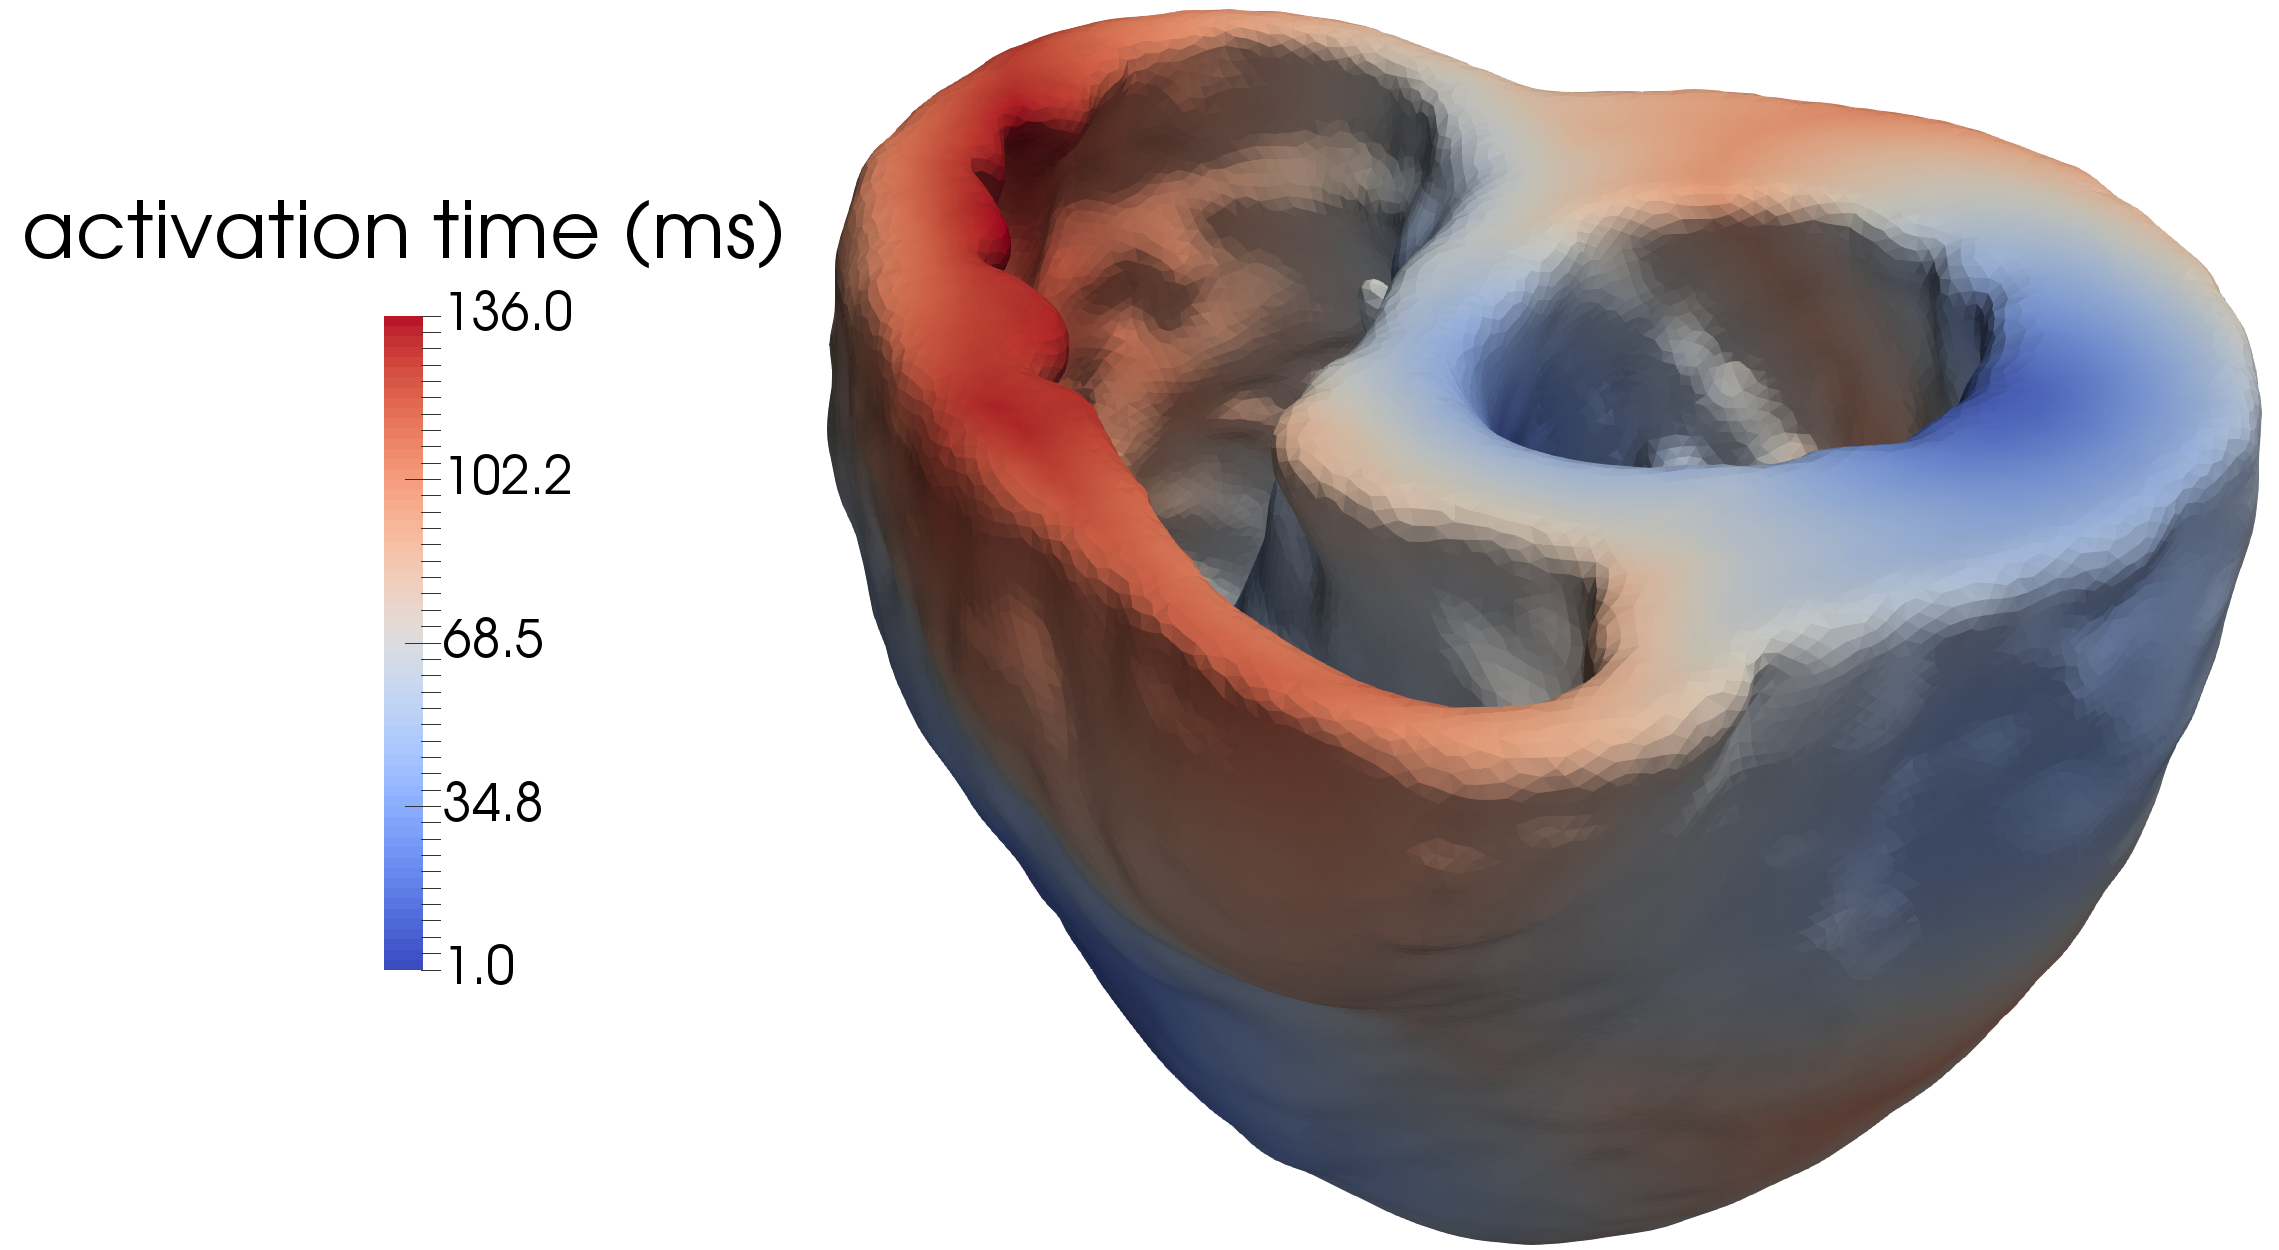
\includegraphics[scale=0.11]{media/4-cardioid/22-activationtime.png}
\label{fig:supp1}}
\subfigure[]{%
		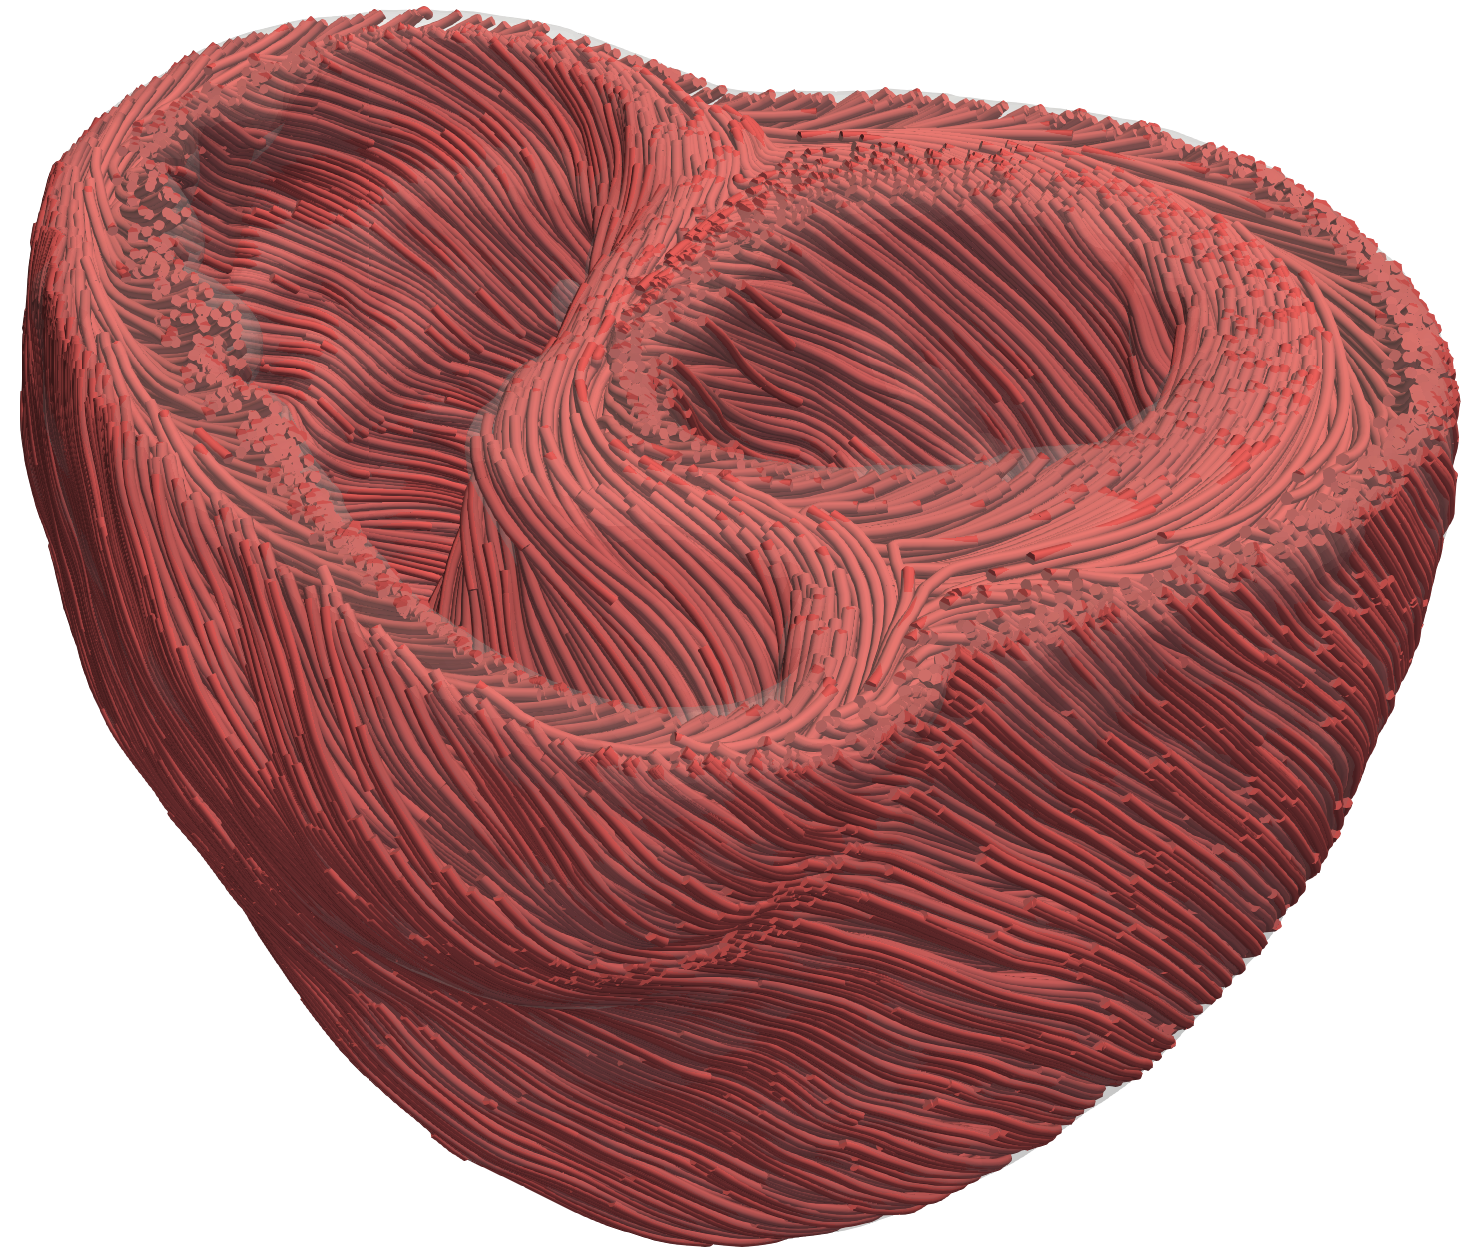
\includegraphics[scale=0.11]{media/4-cardioid/3-fibers.png}
\label{fig:supp2}}
\subfigure[]{%
		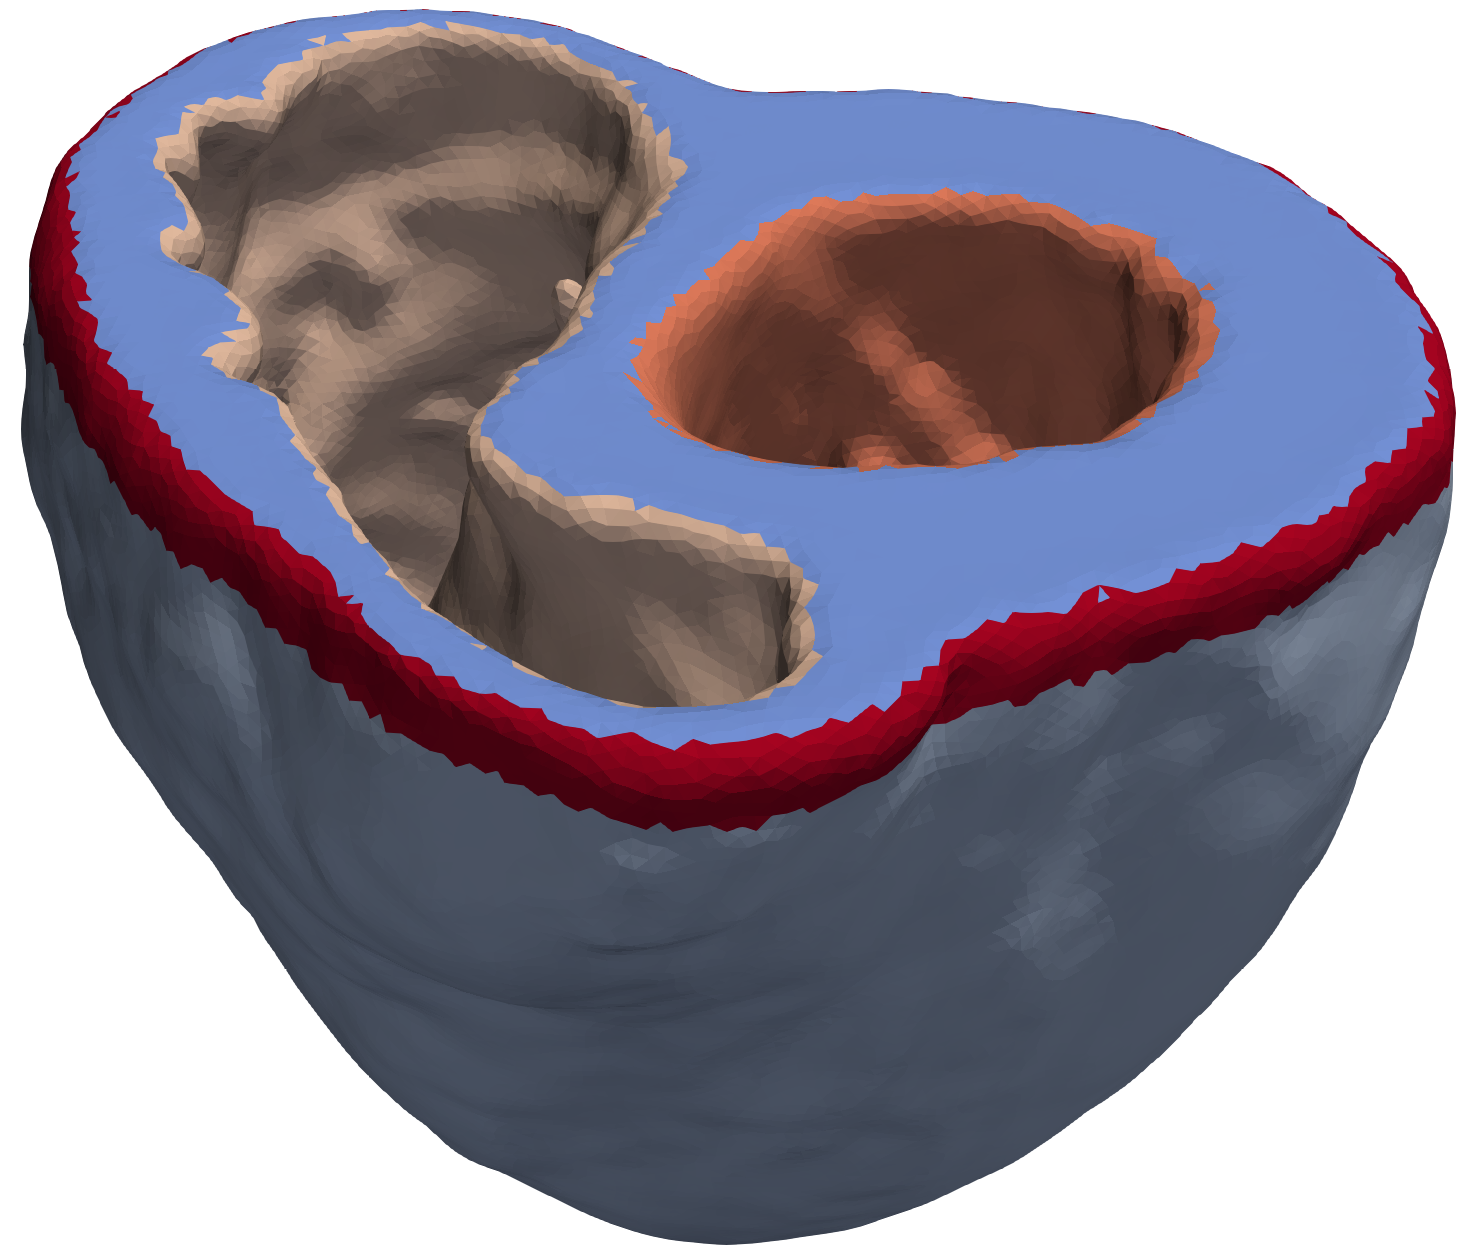
\includegraphics[scale=0.11]{media/4-cardioid/4-tagged.png}
\label{fig:supp3}}
%
\caption{Mechanics modeling considerations: (a) electrical activation times, (b) muscle fiber orientations, and c) surface tagging and prescription of corresponding boundary conditions.}
\label{fig:supp}
\end{sidewaysfigure}

\textbf{Fiber Generation}

Both the passive and active portions of the constitutive model depend on the muscle fiber orientation. Fiber orientations may be generated directly from DTMRI data, but that process requires denoising, smoothing, and interpolating tensor datasets, which can lead to unsatisfactory results. Additionally, DTMRI data is more expensive to acquire, and may not always be available. The Cardioid fiber generation code opts for the more popular \textit{rule-based approach}, in which fiber orientations are artificially generated based on the input mesh to mimic the actual muscle fiber orientations. The code utilizes the algorithm by Bayer \textit{et al.}~\cite{bayer_2012}, which involves solving Laplace's equation $\nabla^2\phi = 0$ four times, each with different Dirichlet boundary conditions (see~\figref{bayer}).

\begin{figure}[ht]
\centering
		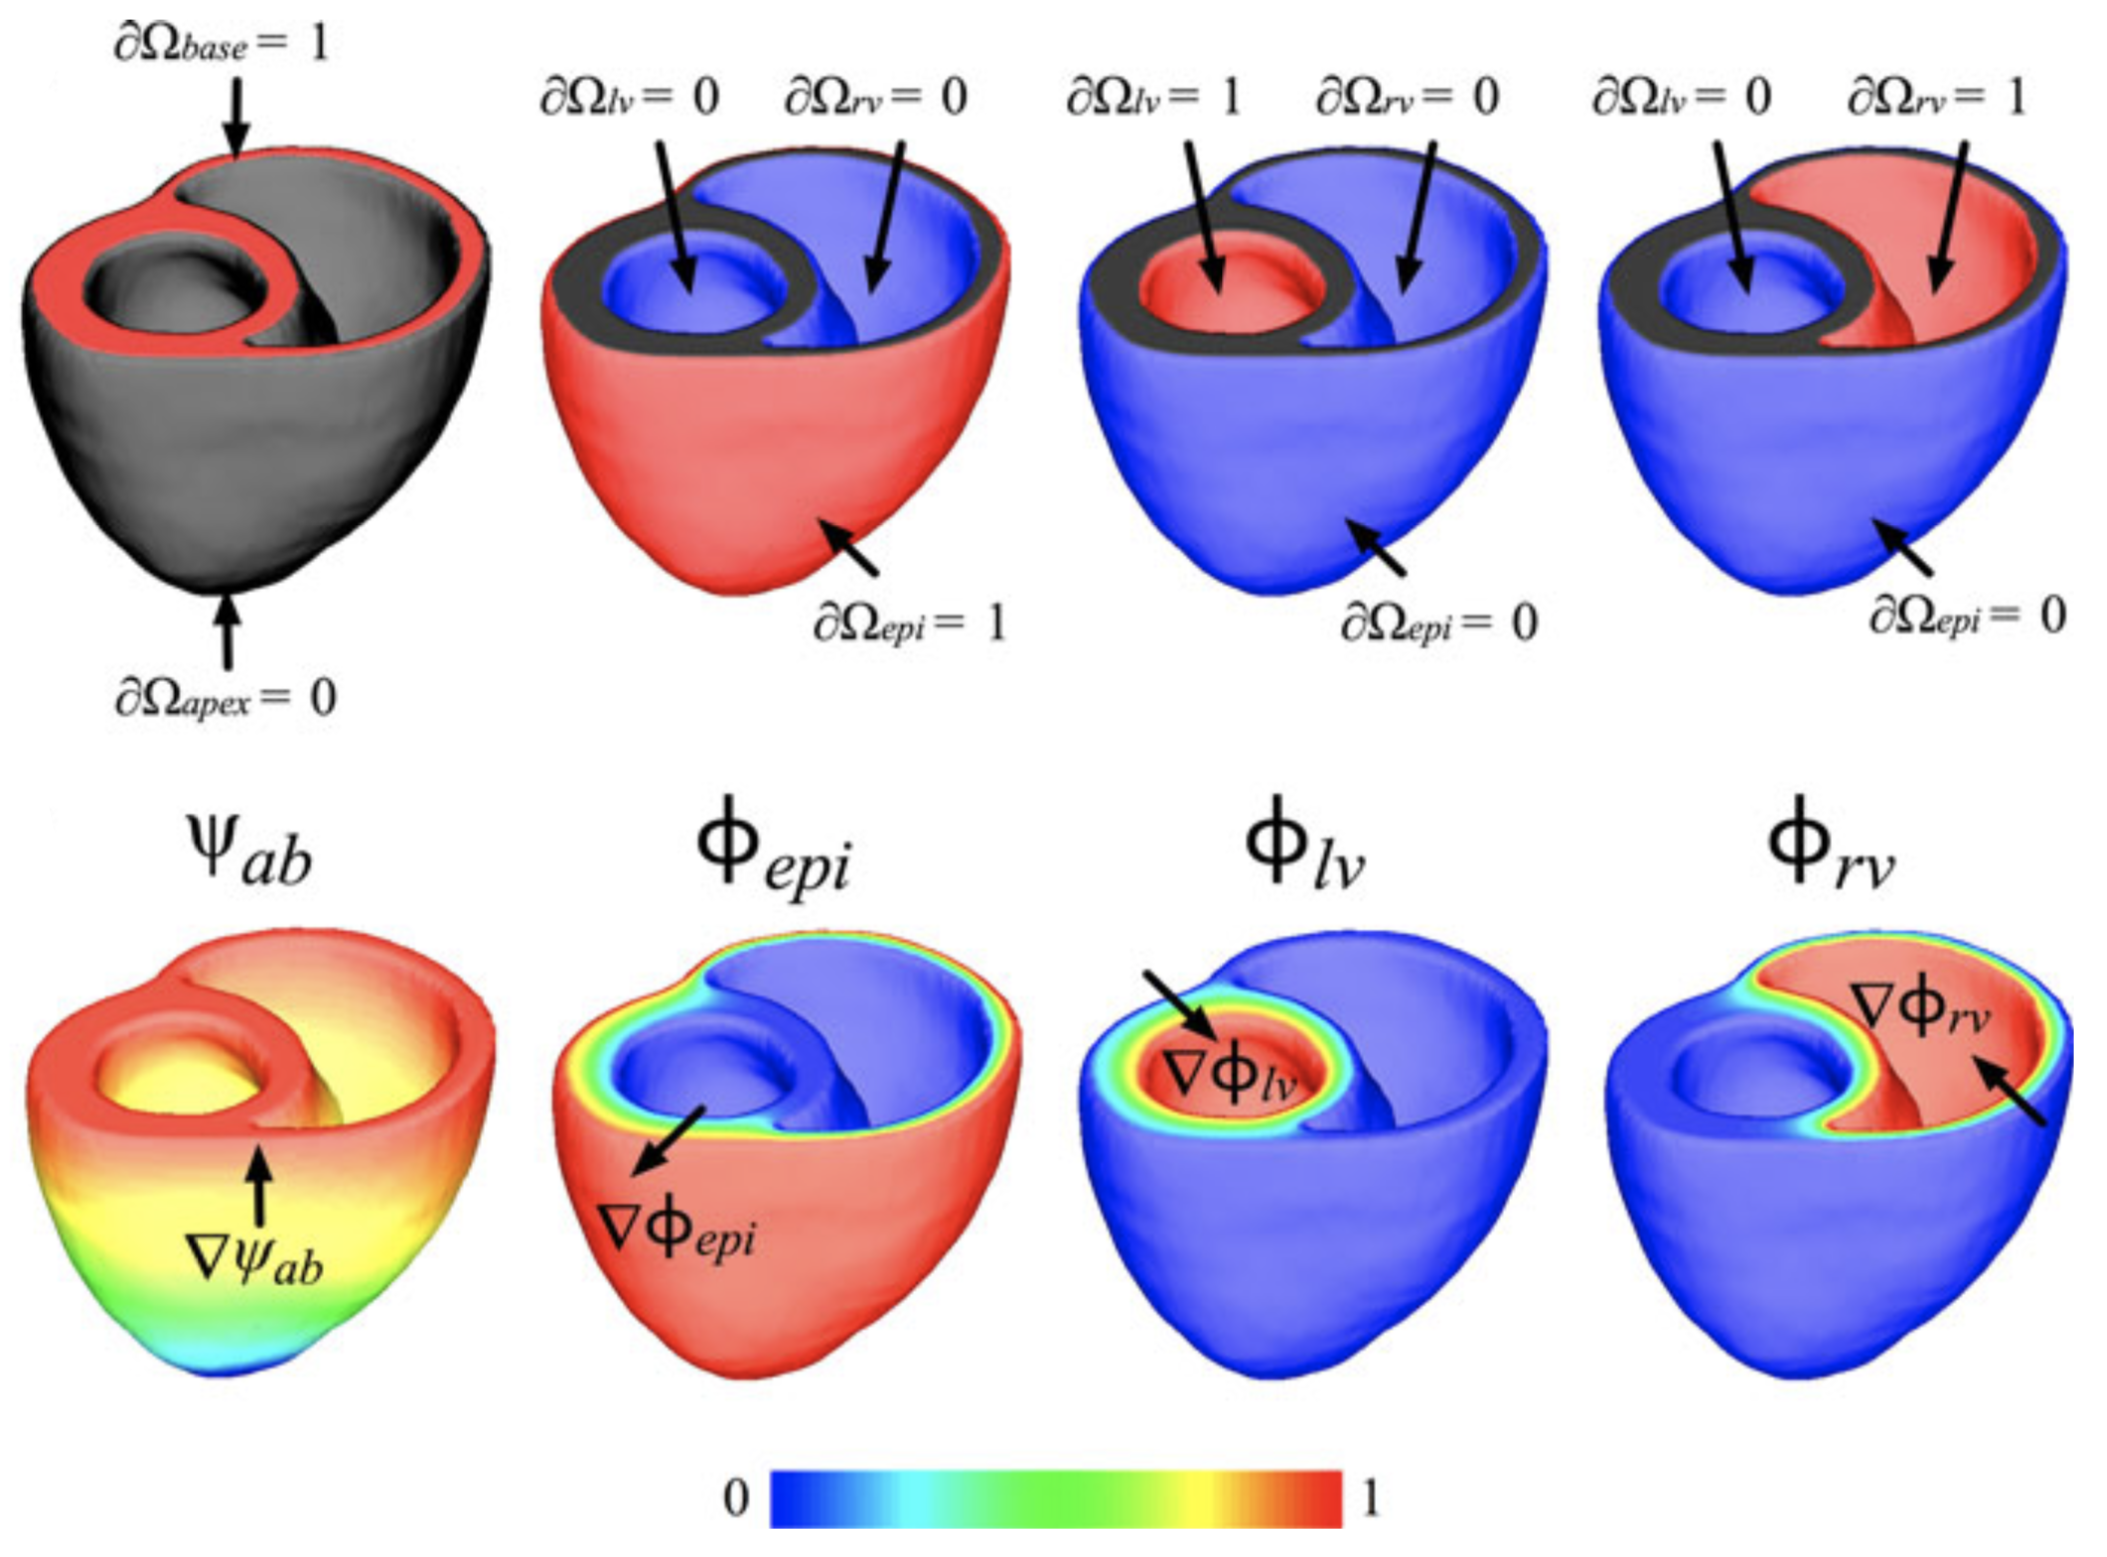
\includegraphics[scale=0.3]{media/bayer.png}
\caption{Boundary conditions and resulting scalar solutions to Laplace's equation. The gradients of the solutions are used to construct the rule-based fiber orientations~\cite{bayer_2012}}
\label{fig:bayer}
\end{figure}

The gradients of these solutions inform the construction of orthotropic fiber orientations at each solution point. Fiber orientations are then interpolated at the junctions between the LV, RV, and septum to ensure that the fiber direction changes smoothly and continuously throughout the entire myocardium. The details by which the gradients are used to construct the fiber orientations and by which orientations are interpolated are explained in Bayer~\textit{et al.}~\cite{bayer_2012}. The Laplace solves are performed using the highly parallelized finite element code \textit{MFEM}~\cite{mfem-library} on the same input quadratic tetrahedral mesh to be used for the mechanics simulation. The algorithm performs robustly for various geometries and compares well with fiber orientations generated directly from DTMRI data. The computed fiber orientations for the mesh of interest are shown in \figref{supp2}.

%%%%%%%%%%%%%%%%%%%%%%%%%%%%%%%%%%%%%%%%%%%%%%%
%%%%%%%%%%%%%%%%%%%%%%%%%%%%%%%%%%%%%%%%%%%%%%%
\subsubsection{Boundary Conditions}
\label{Boundary Conditions}

Fluid flow and fluid-structure interaction are not yet implemented in the Cardioid code, so a volume constraint is imposed to mimic the effect of blood flow in the ventricles. The volumes of the ventricle cavities are calculated based on a lumped circulatory model by Kerckhoffs \textit{et al.}~\cite{kerckhoffs_2006}, which are in turn used to determine the time-varying, solution-dependent pressure boundary conditions.

A system of coupled ODEs describing the time evolution of the left ventricle volume $V_{LV}$ and the right ventricle volume $V_{RV}$ for the circulatory model can be written in the form:
\begin{align}
\frac{d\bm{w}_{c}}{dt} = \bm{q}_c(\bm{w}_c, p_{LV}, p_{RV}; t) \\
\frac{dV_{LV}}{dt} = g_{LV}(p_{LV}, \bm{w}_c; t) \\
\frac{dV_{RV}}{dt} = g_{RV}(p_{RV}, \bm{w}_c; t)
\end{align}
where $\bm{w}_c$ is the vector of state variables for the circulatory model, $p_{LV}$ and $p_{RV}$ are the  pressures inside the left and right ventricles, and $\frac{dV_{LV}}{dt}$ and $\frac{dV_{RV}}{dt}$ represent the change in blood volume into the each of the ventricles. The right hand side functions $\bm{q}_c$, $g_{LV}$, and $g_{RV}$ are described in detail in Kerckhoffs~\textit{et al.}~\cite{kerckhoffs_2006}. This paradigm assumes both that the blood is incompressible, and that the pressure is uniform within each ventricle. For each time step, the ventricular volumes are calculated from the circulatory model and imposed as constraints on the finite element mesh to determine the corresponding ventricular pressures. The details by which the pressures are computed from the volume constraint are detailed in Gurev~\textit{et al.}~\cite{gurev_2015}. The circulatory model is shown in~\figref{bcs}.
\begin{figure}[ht]
\centering
		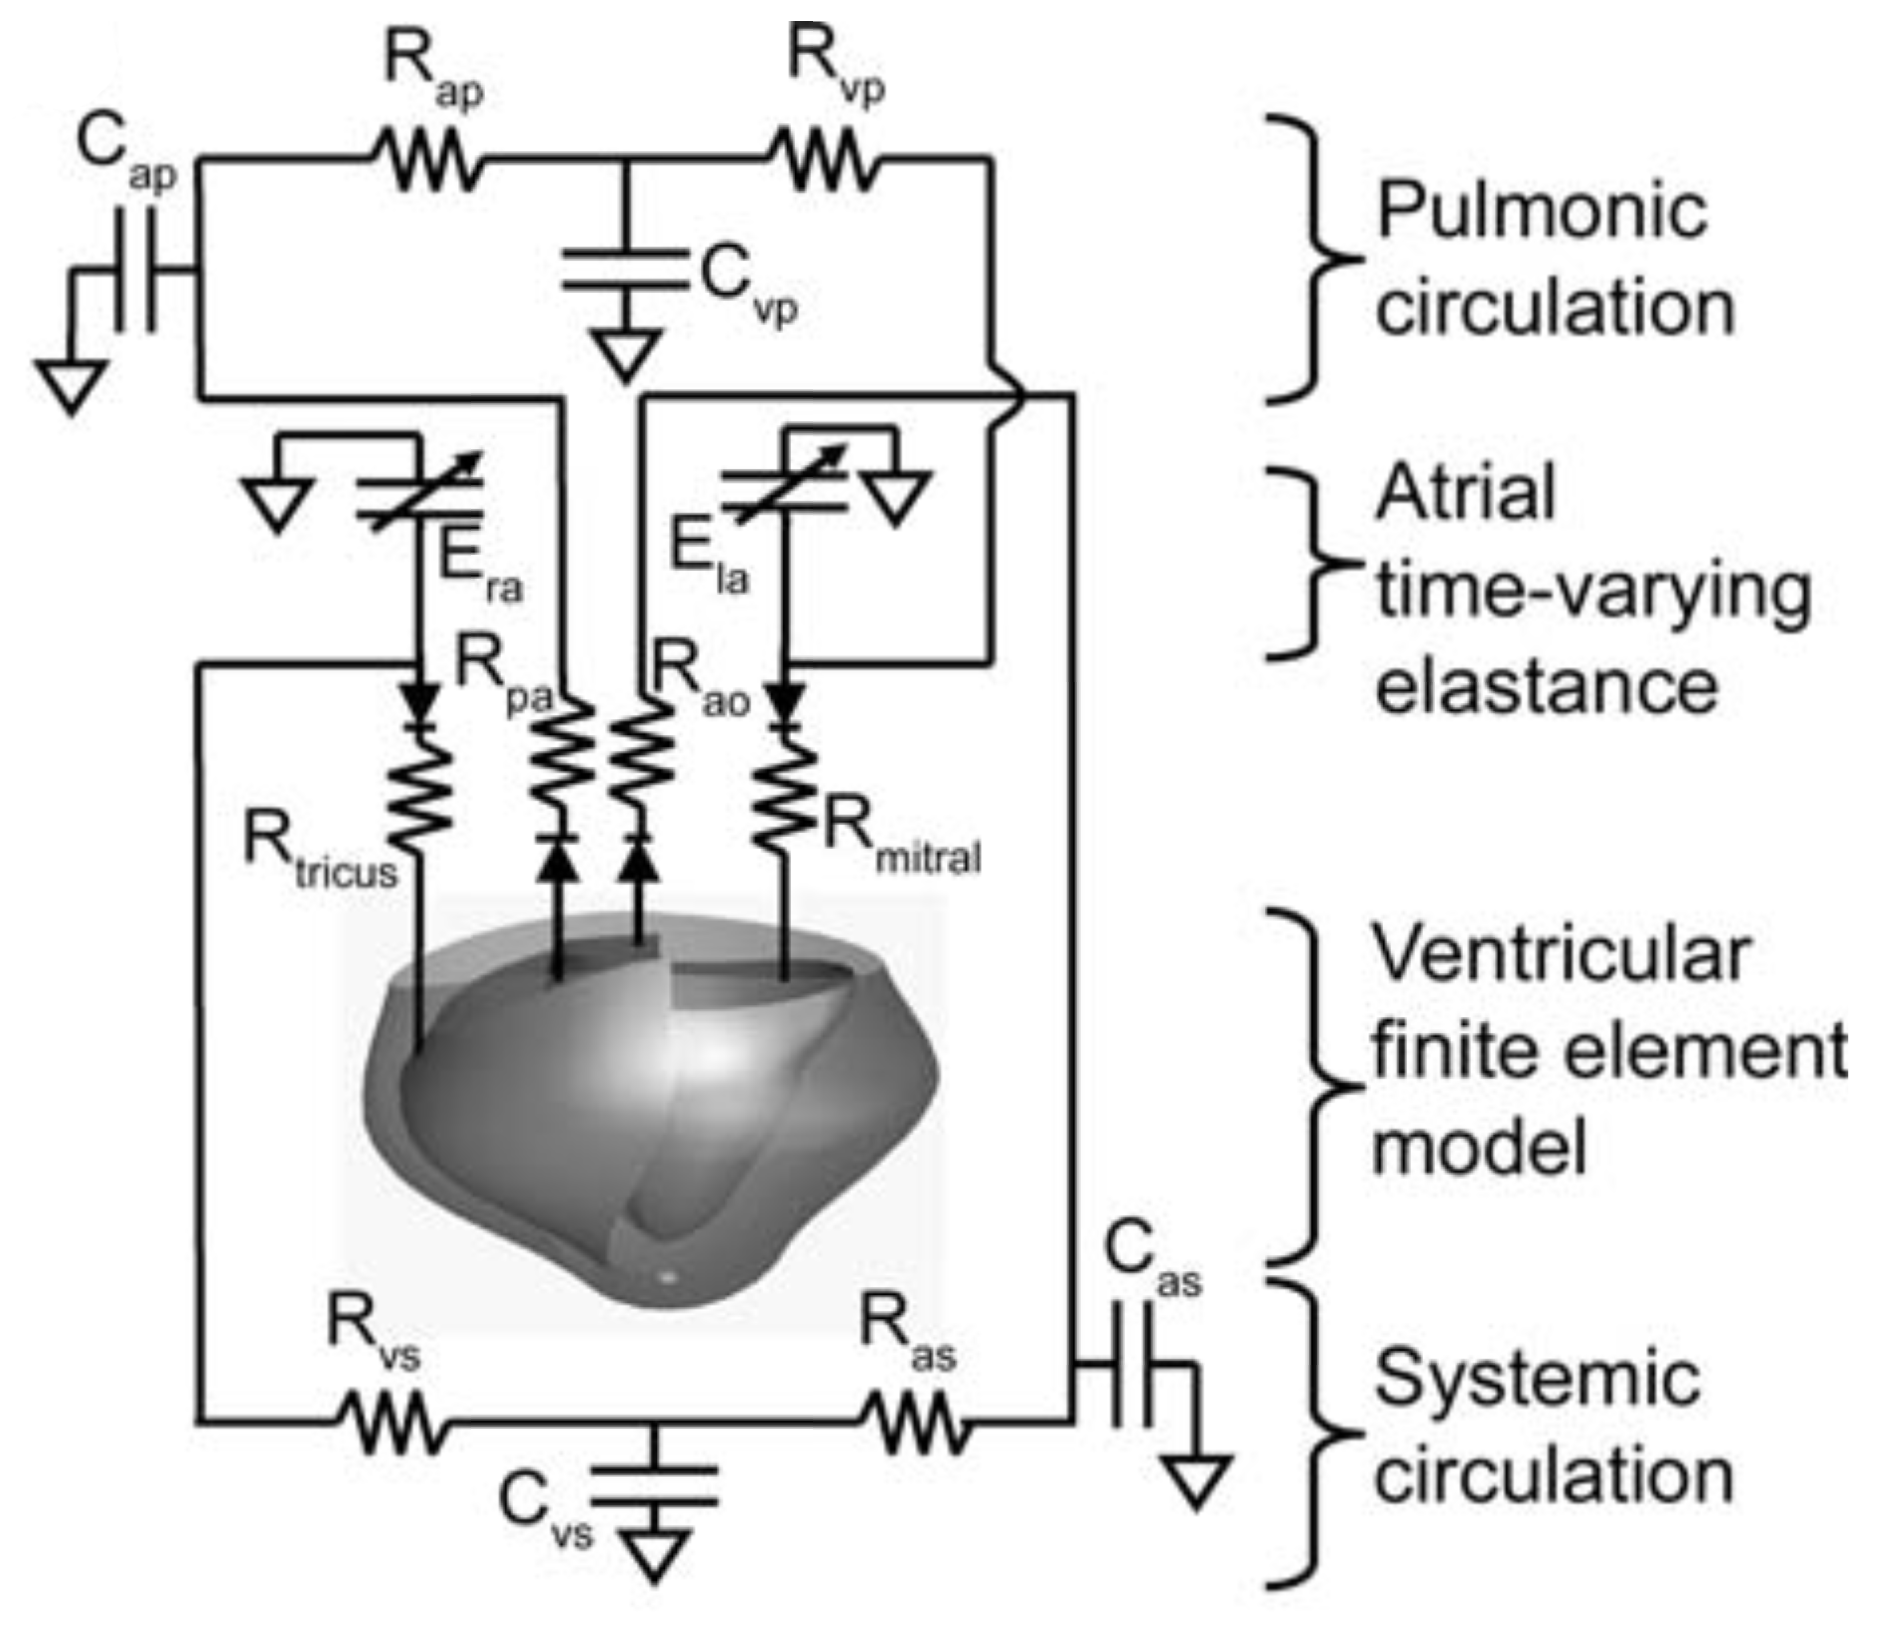
\includegraphics[scale=0.3]{media/bcs.png}
\caption{Lumped circulatory model of Kerckhoffs\textit{et al.}~\cite{kerckhoffs_2006}. Variables shown in the schematic are parameters in the coupled system of ODEs that are solved for ventricular volumes.}
\label{fig:bcs}
\end{figure}

In order to avoid highly nonlinear solutions at the beginning of the simulation, initial pressures are applied linearly in the first 100 ms prior to ``turning on'' the active contraction. One may think of the first 100 ms as a period in which a residual stress is applied prior to imposing the loading and boundary conditions of interest for the remainder of the simulation.

Displacement boundary conditions are enforced such that the base of the heart is not allowed to move out of plane, and that a strip of the epicardium near the base experiences zero displacements in all directions. In order to enforce these displacement and pressure BCs, the appropriate surfaces must be identified. Identification of the base, epicardium, left ventricle, and right ventricle is actually a necessary intermediate step in generating fiber directions, so those boundary condition tags are already available (see~\figref{supp3}).

%%%%%%%%%%%%%%%%%%%%%%%%%%%%%%%%%%%%%%%%%%%%%%%
%%%%%%%%%%%%%%%%%%%%%%%%%%%%%%%%%%%%%%%%%%%%%%%
\subsubsection{Solver}
\label{Solver}

The quadratic tetrahedral mesh described previously is used together with the material model and boundary conditions to perform conventional finite element simulations using the freely available \textit{oomph-lib}~\cite{oomph}. 

In the interest of solving problems with fine discretizations, Gurev \textit{et al.} avoid direct solvers of the linear system in Cardioid due to their poor scalability. Instead they employ a Krylov subspace iterative solver, which is more suitable for large scalable problems. The existence of active contraction creates saddle-points in the linear system that are addressed with a novel preconditioner. The details of the linear solver may be found in the publication by Gurev \textit{et al.}.

The simulation was performed on the \textit{Surface} computing platform at Lawrence Livermore National Laboratory. The Moab schedule manager was used to submit the job to be run on 50 nodes, with 16 cores per node, for a total of 800 processes. With an assumed beat duration of 1000 $ms$ for a healthy human heart (i.e., 60 beats per minute), the simulation is run from time 0 to 5100 ms with a time increment $\Delta t = 1 ms$. The simulation completed roughly one heartbeat per 24 hours of wall clock time. As mentioned previously, the first 100 ms are used to linearly apply the initial pressures for the simulation. The first beat is discarded as the heart reaches a dynamic steady state, and thus four full beats of a healthy human heart are extracted from the results.

%%%%%%%%%%%%%%%%%%%%%%%%%%%%%%%%%%%%%%%%%%%%%%%
%%%%%%%%%%%%%%%%%%%%%%%%%%%%%%%%%%%%%%%%%%%%%%%
\subsection{Results}
\label{Results}

Simulation results for the problem described in this chapter are shown in~\figref{pv} and~\figref{snaps}. \figref{pv1} is known as a \textit{P-V loop} of the left ventricle, and \figref{pv2} is a time history plot of the pressure in the left and right ventricles. \figref{pv1} demonstrates the four stages of the cardiac cycle: 1) isovolumetric contraction from label a to b, ventricular ejection of blood from label b to c, isovolumetric relaxation from label c to d, and ventricular filling from label d to a. Isovolumetric contraction and ventricular ejection comprise what is known as \textit{systole}, in which the ventricles are contracting, whereas isovolumetric relaxation and ventricular filling are known as \textit{diastole}, in which the ventricles are relaxing. The labels in \figref{pv1} correspond to the panels in~\figref{snaps} showing the deformed mesh with an overlay of fiber stretch $\lambda$. During a cycle, fiber stretch ranges from 0.6 to 1.4, certainly justifying the finite deformation simulatoin approach. The results closely match those in Gurev~\textit{et al.}~\cite{gurev_2015}, in which a different heart geometry and electrophysiology is used, indicating a robustness to the workflow. The full video of four heartbeats played at one quarter speed may be found at \href{youtu.be/RtQKEjdR4MU}. A robust workflow has thus been demonstrated for performing bi-ventricular cardiac mechanics simulations. Additional validation of the results, quantitiative metrics for the quality of the solution, and sensitivity studies of the simulation parameters would be the next steps and would certainly be informative.

In the process of performing simulations, the workflow for generating the mesh; generating fiber orientations; running the electrophysiology code to produce activation times; running the mechanics code; and post-processing results was improved, simplified, and further automated via Python scripts. The steps have been rigorously documented, and will directly facilitate the current Cardioid research project involving machine learning, which will require a robust and timely generation of simulation results for large numbers of patient imaging data.

\begin{figure}[ht]
\centering
\subfigure[]{%
		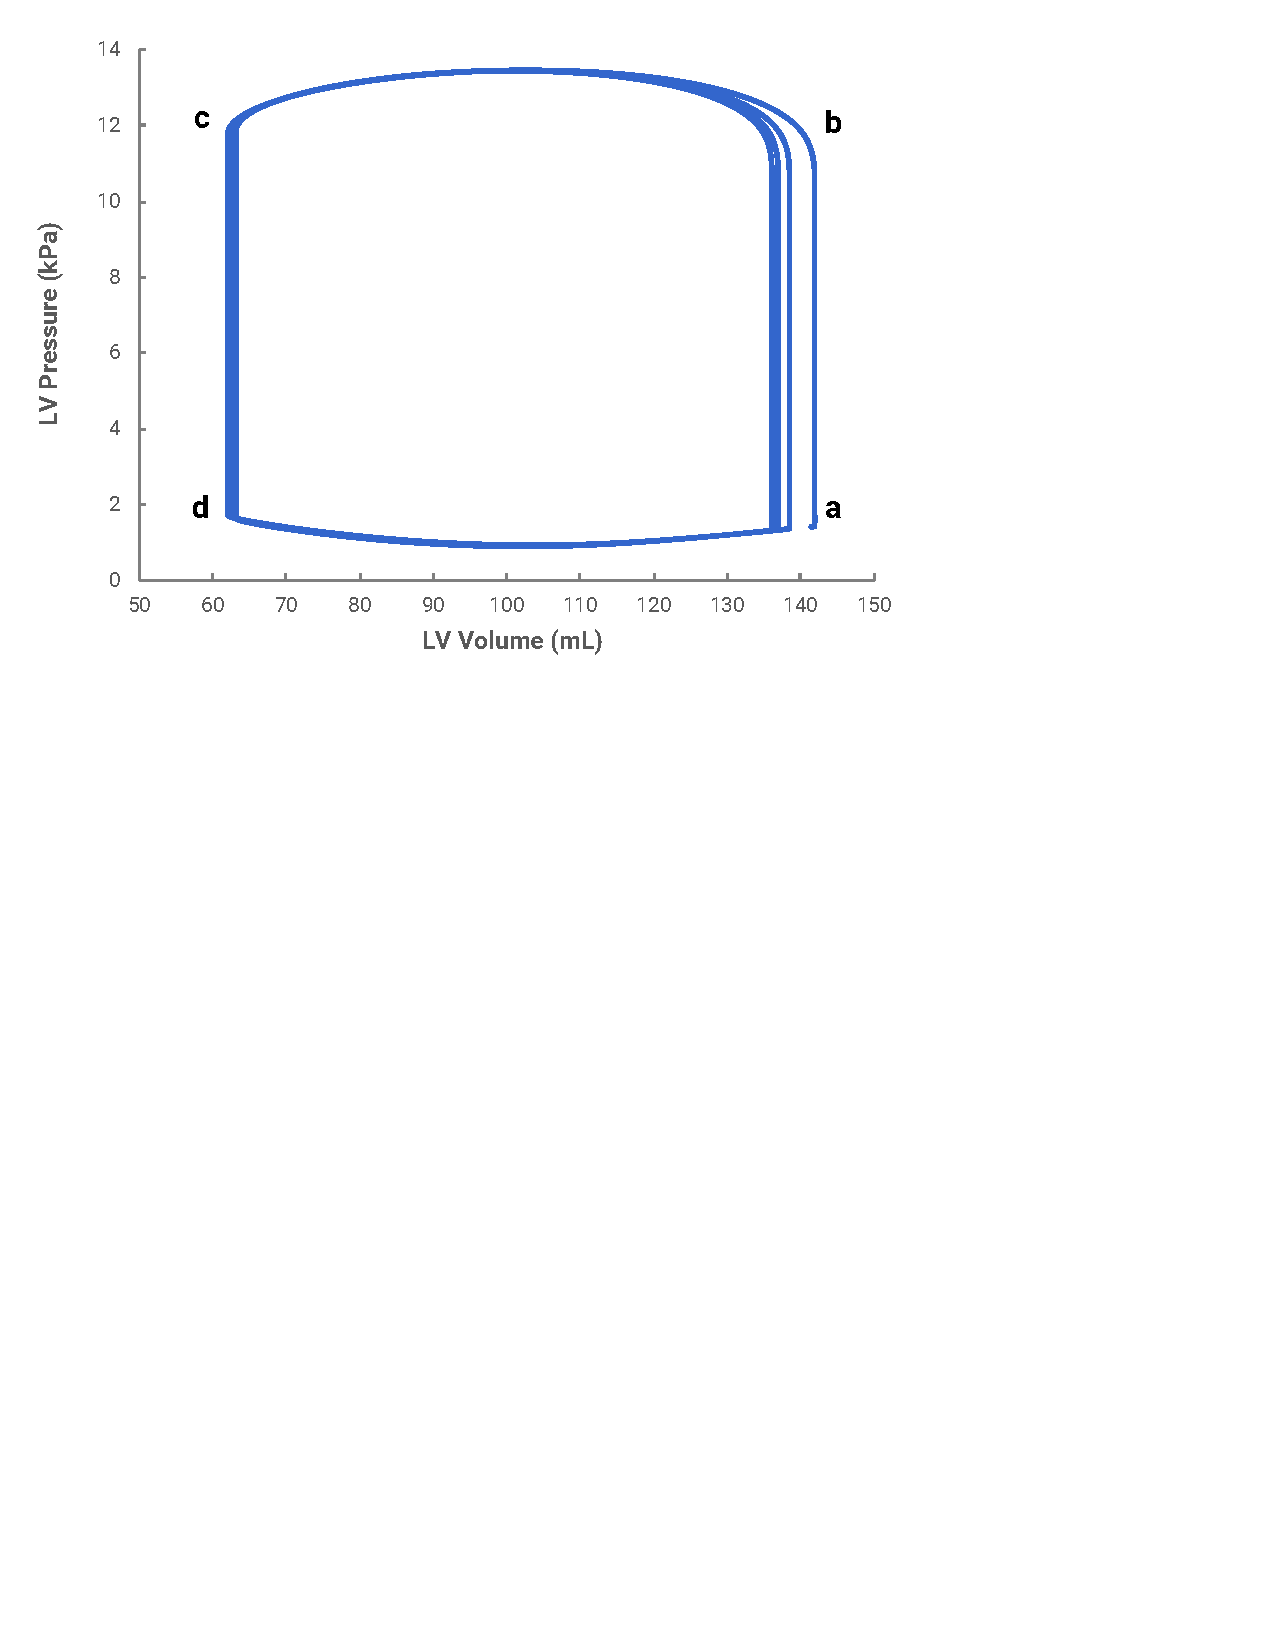
\includegraphics[scale=0.5]{media/4-cardioid/5-pv/pressure_volume-1.pdf}
\label{fig:pv1}}		
\subfigure[]{%
		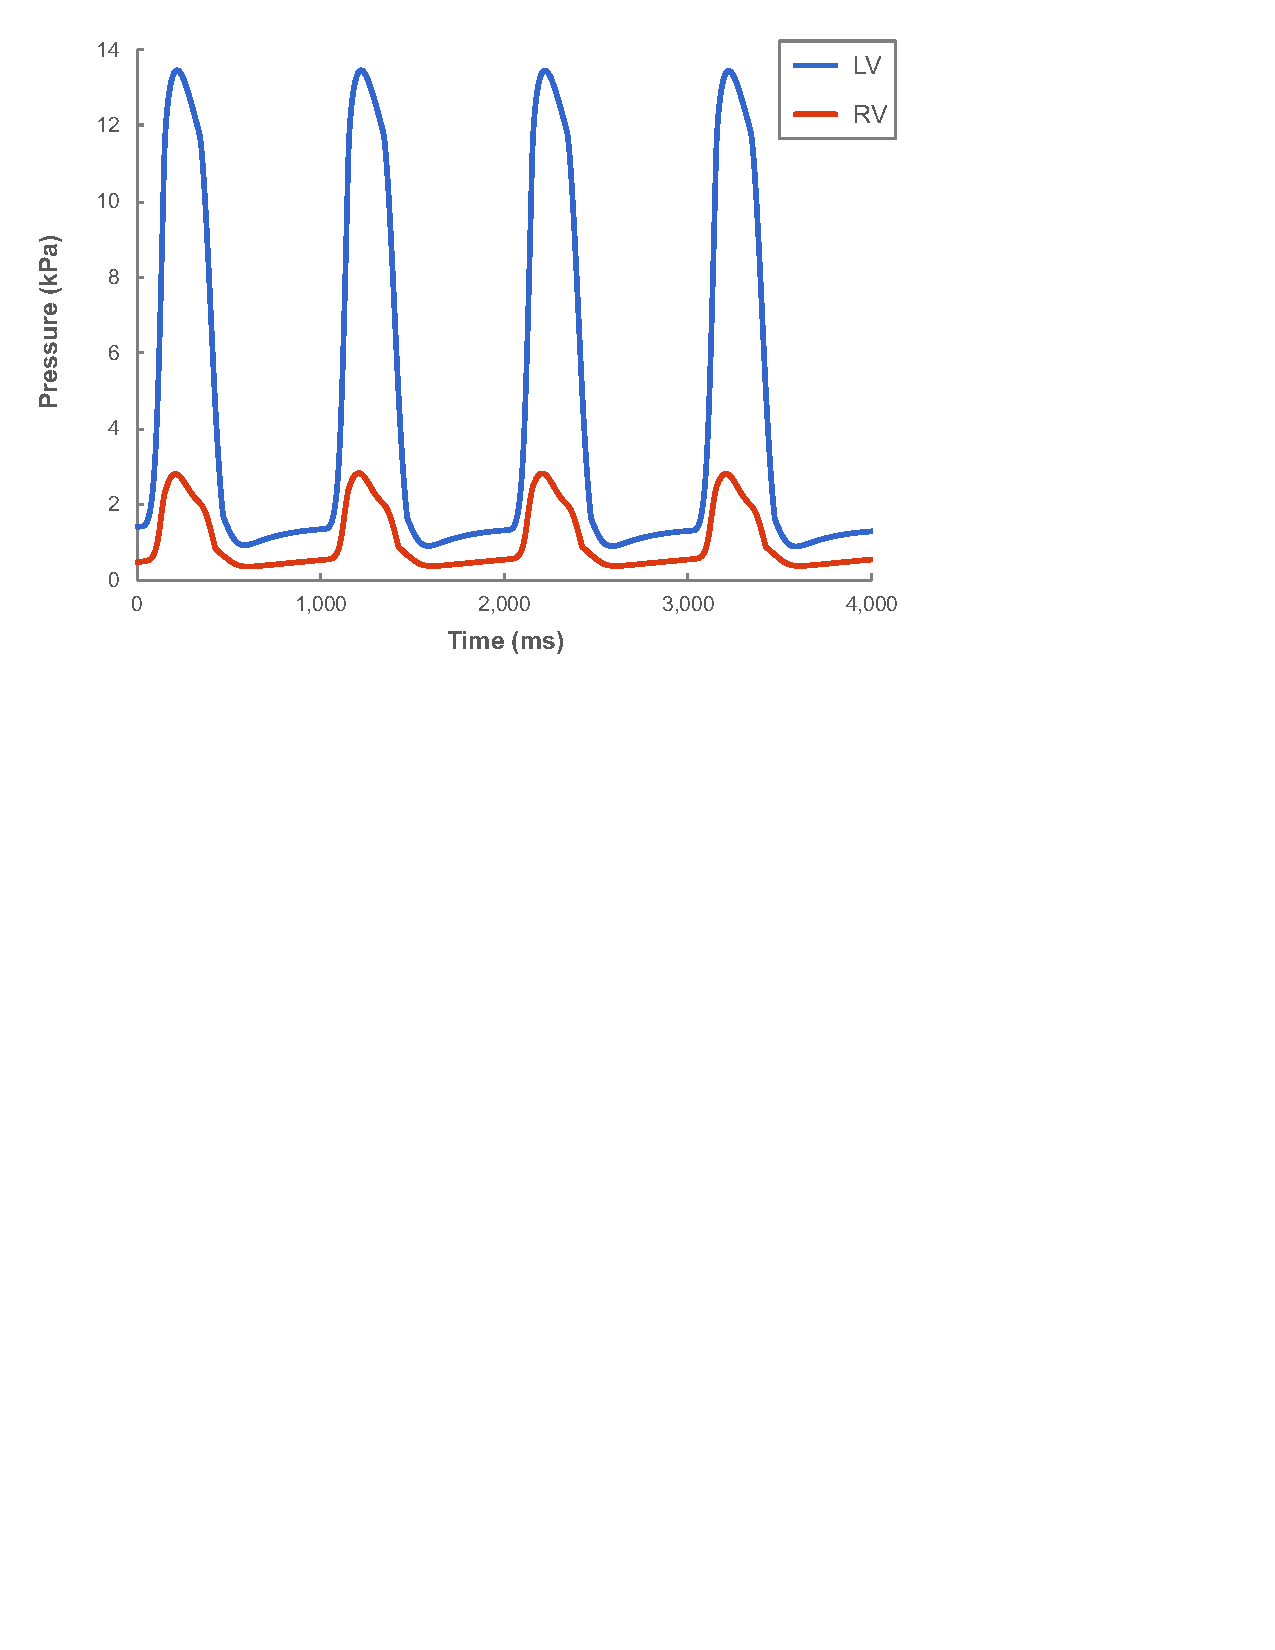
\includegraphics[scale=0.5]{media/4-cardioid/5-pv/pressure_volume-2.pdf}
\label{fig:pv2}}		
%
\caption{Results from Cardioid simulation: (a) P-V loop of left ventricle, (b) pressure time history in left and right ventricles.}
\label{fig:pv}
\end{figure}

\begin{sidewaysfigure}[htbp!]
\centering
\subfigure[]{%
		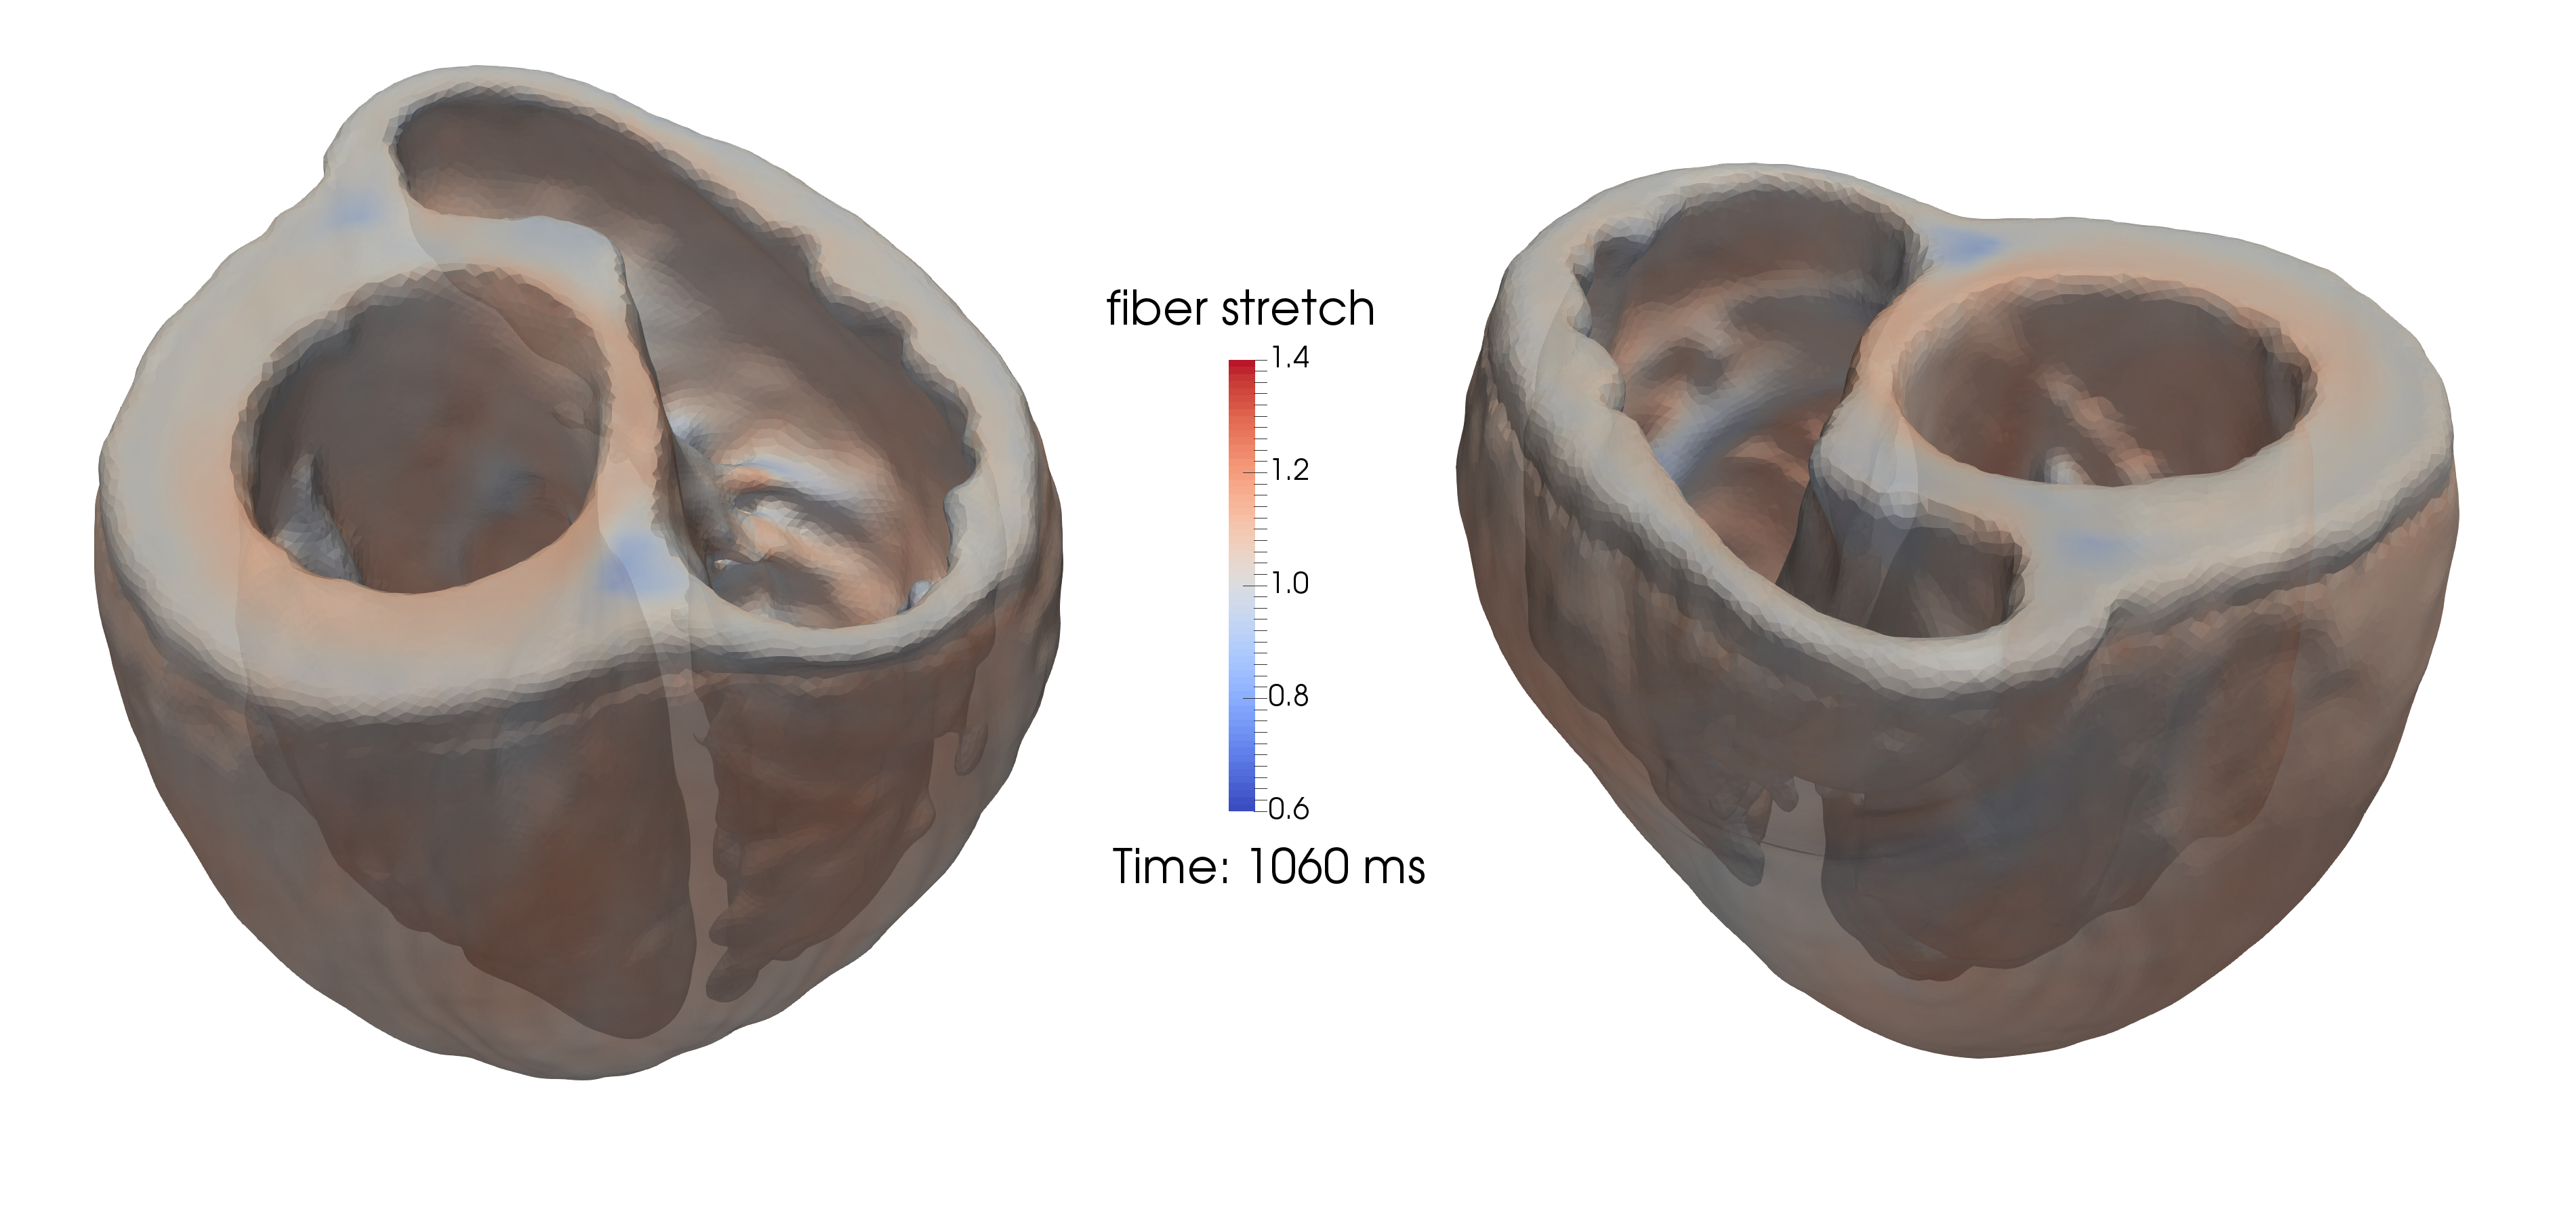
\includegraphics[scale=0.08]{media/4-cardioid/6-vid/a.png}
\label{fig:snaps1}}		
\subfigure[]{%
		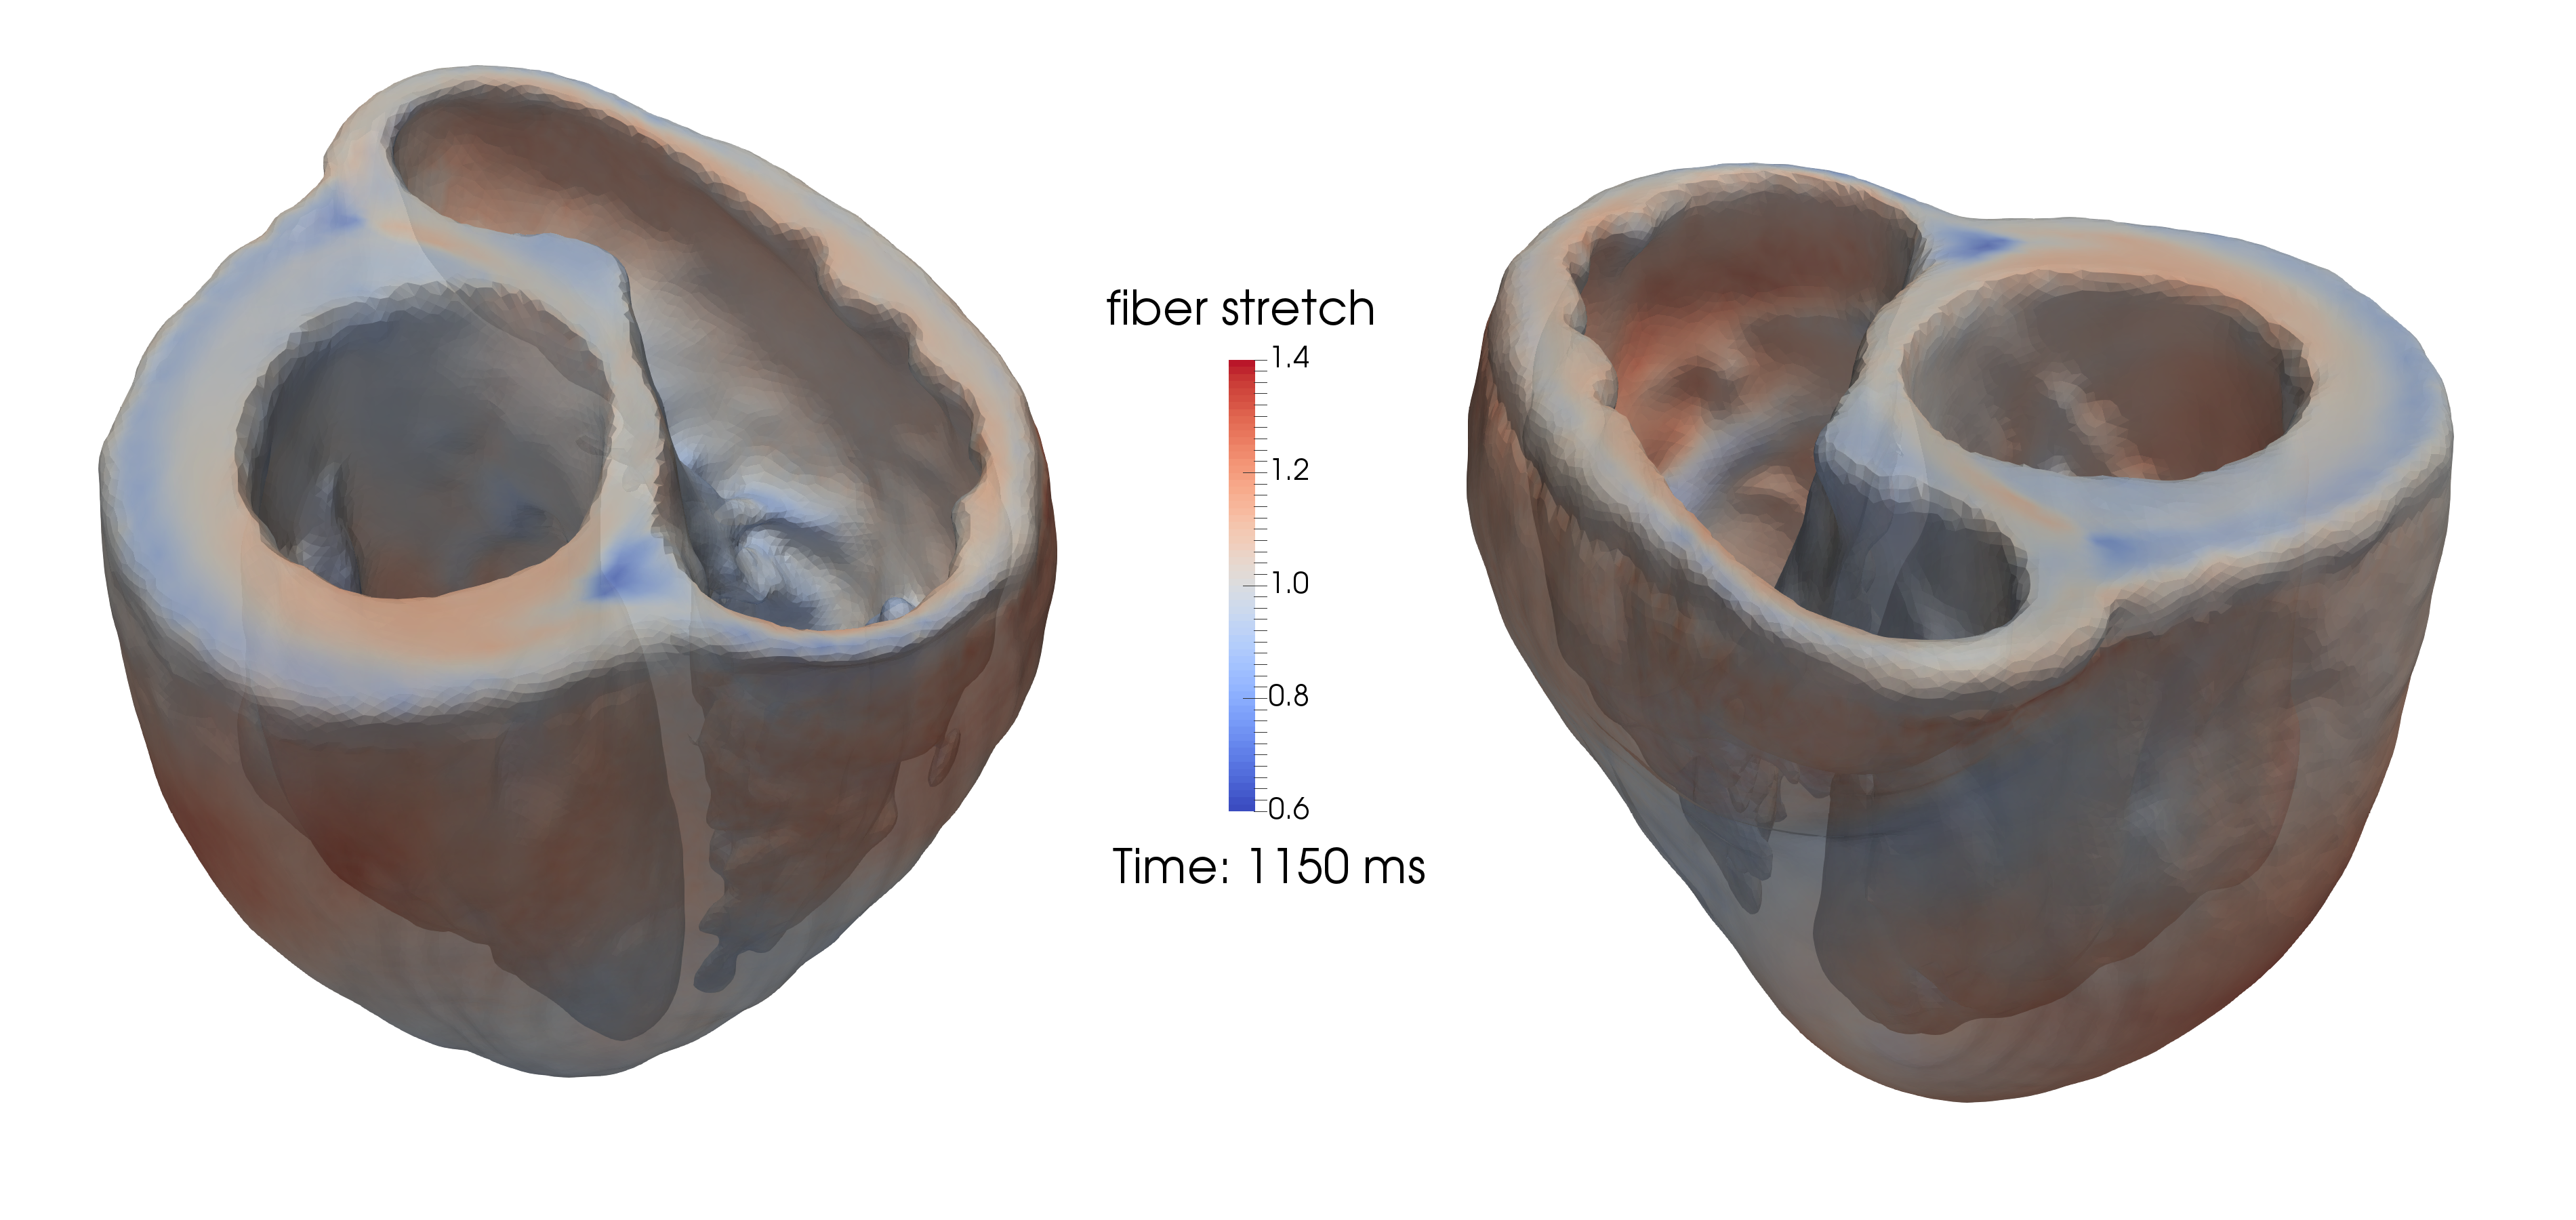
\includegraphics[scale=0.08]{media/4-cardioid/6-vid/b.png}
\label{fig:snaps2}}
\\
\subfigure[]{%
		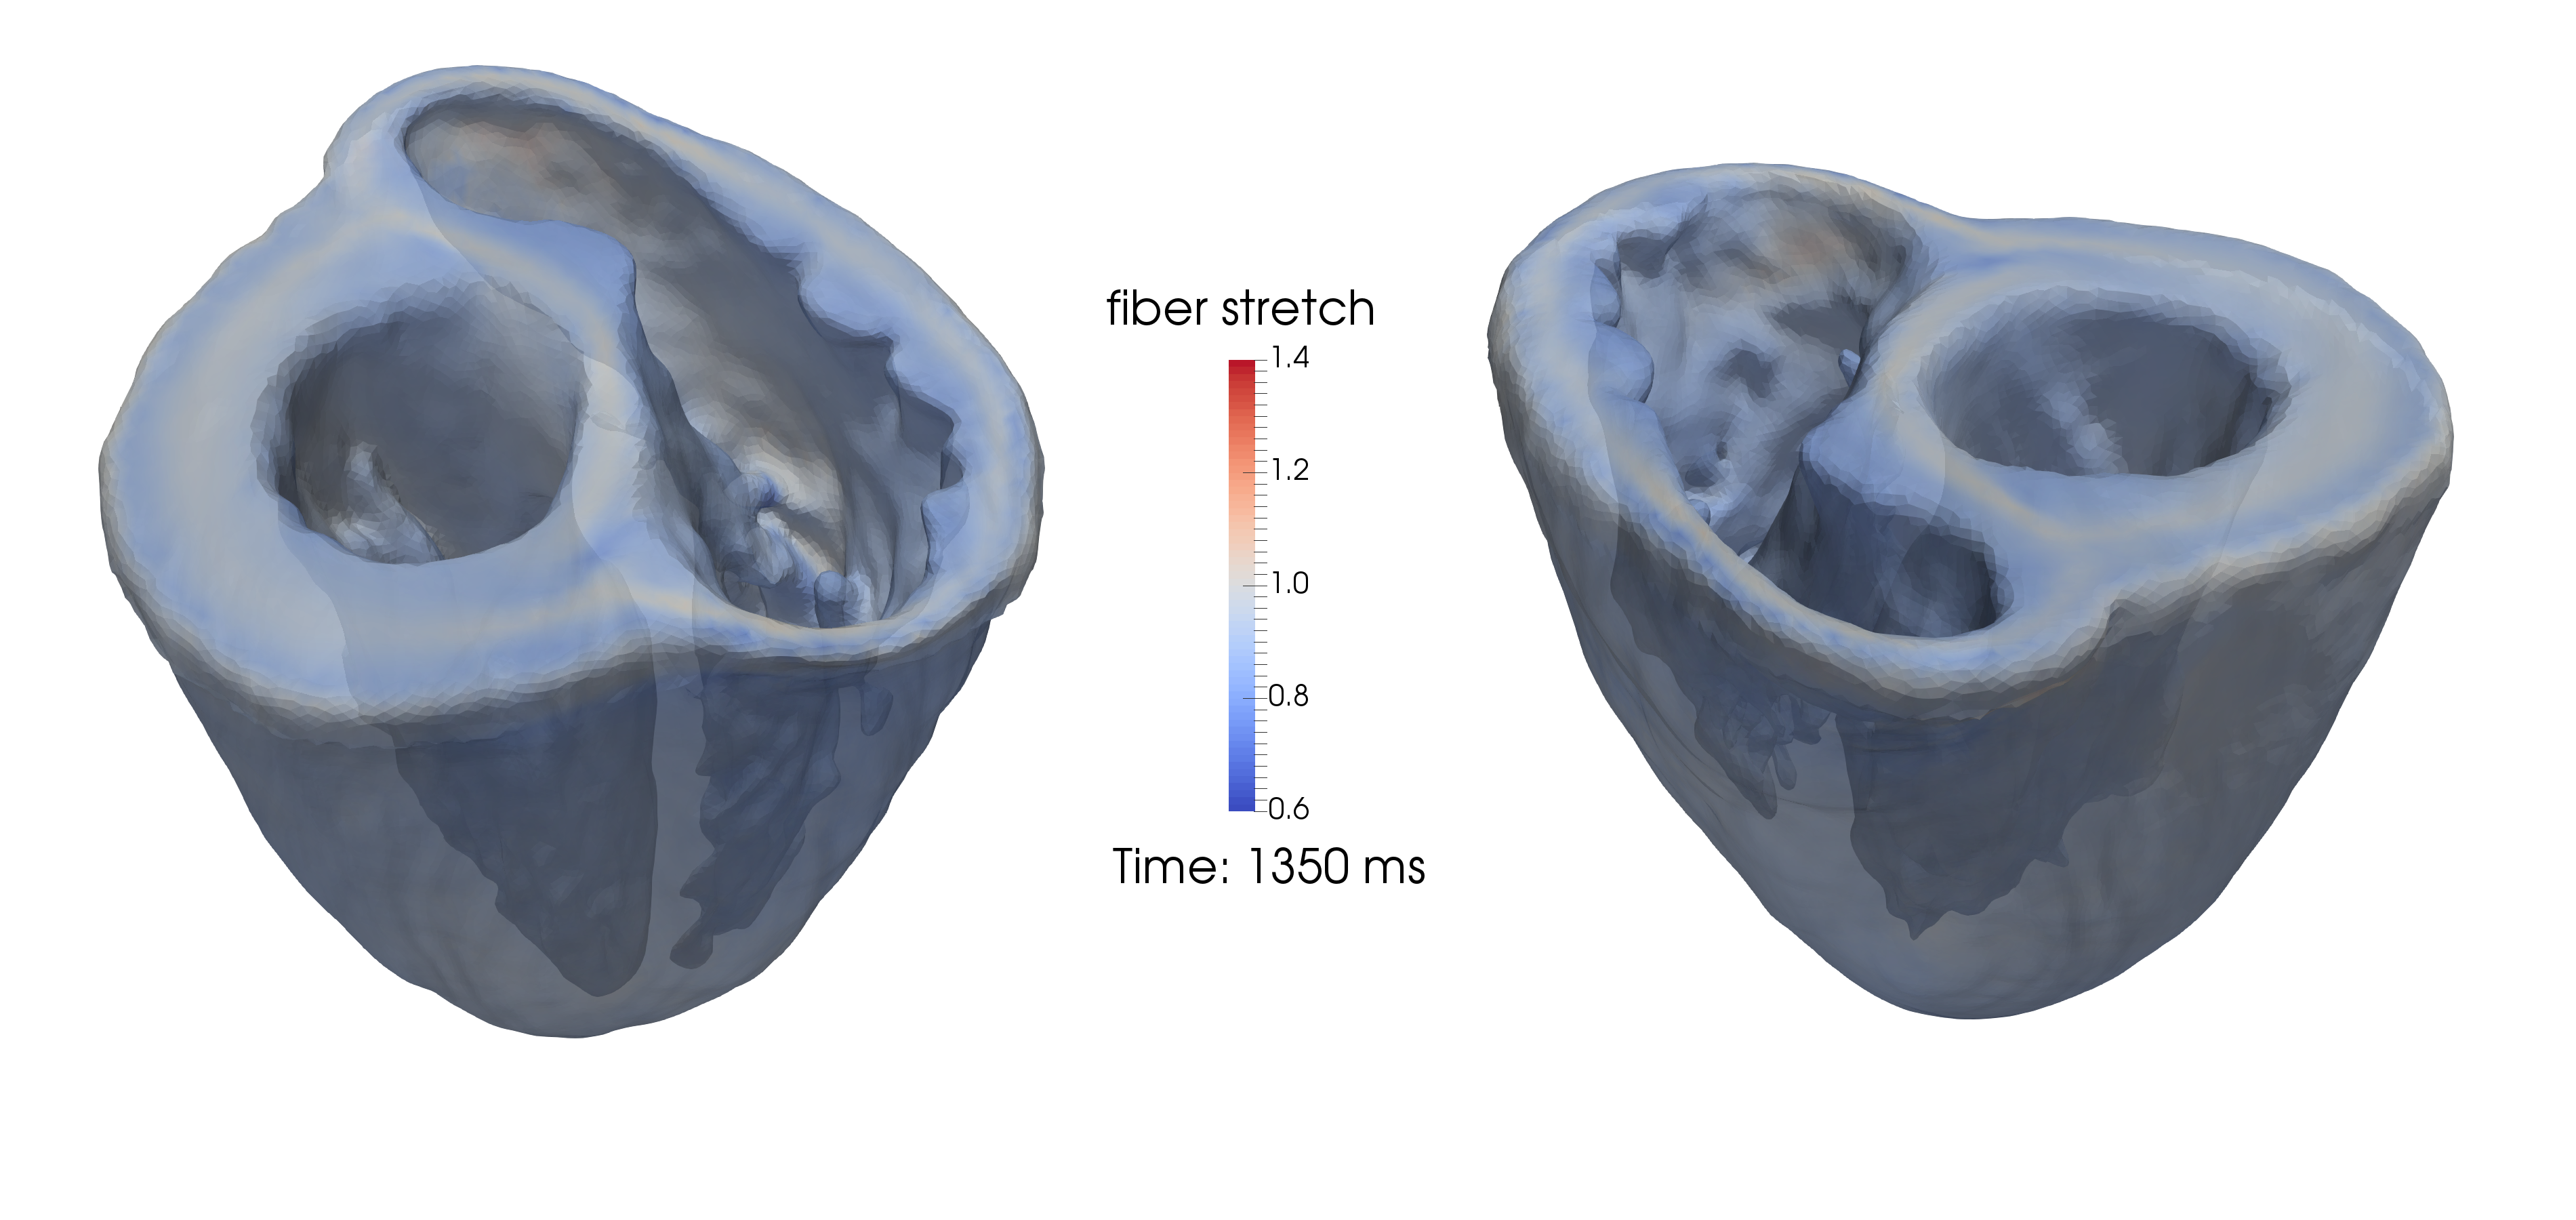
\includegraphics[scale=0.08]{media/4-cardioid/6-vid/c.png}
\label{fig:snapsf3}}		
\subfigure[]{%
		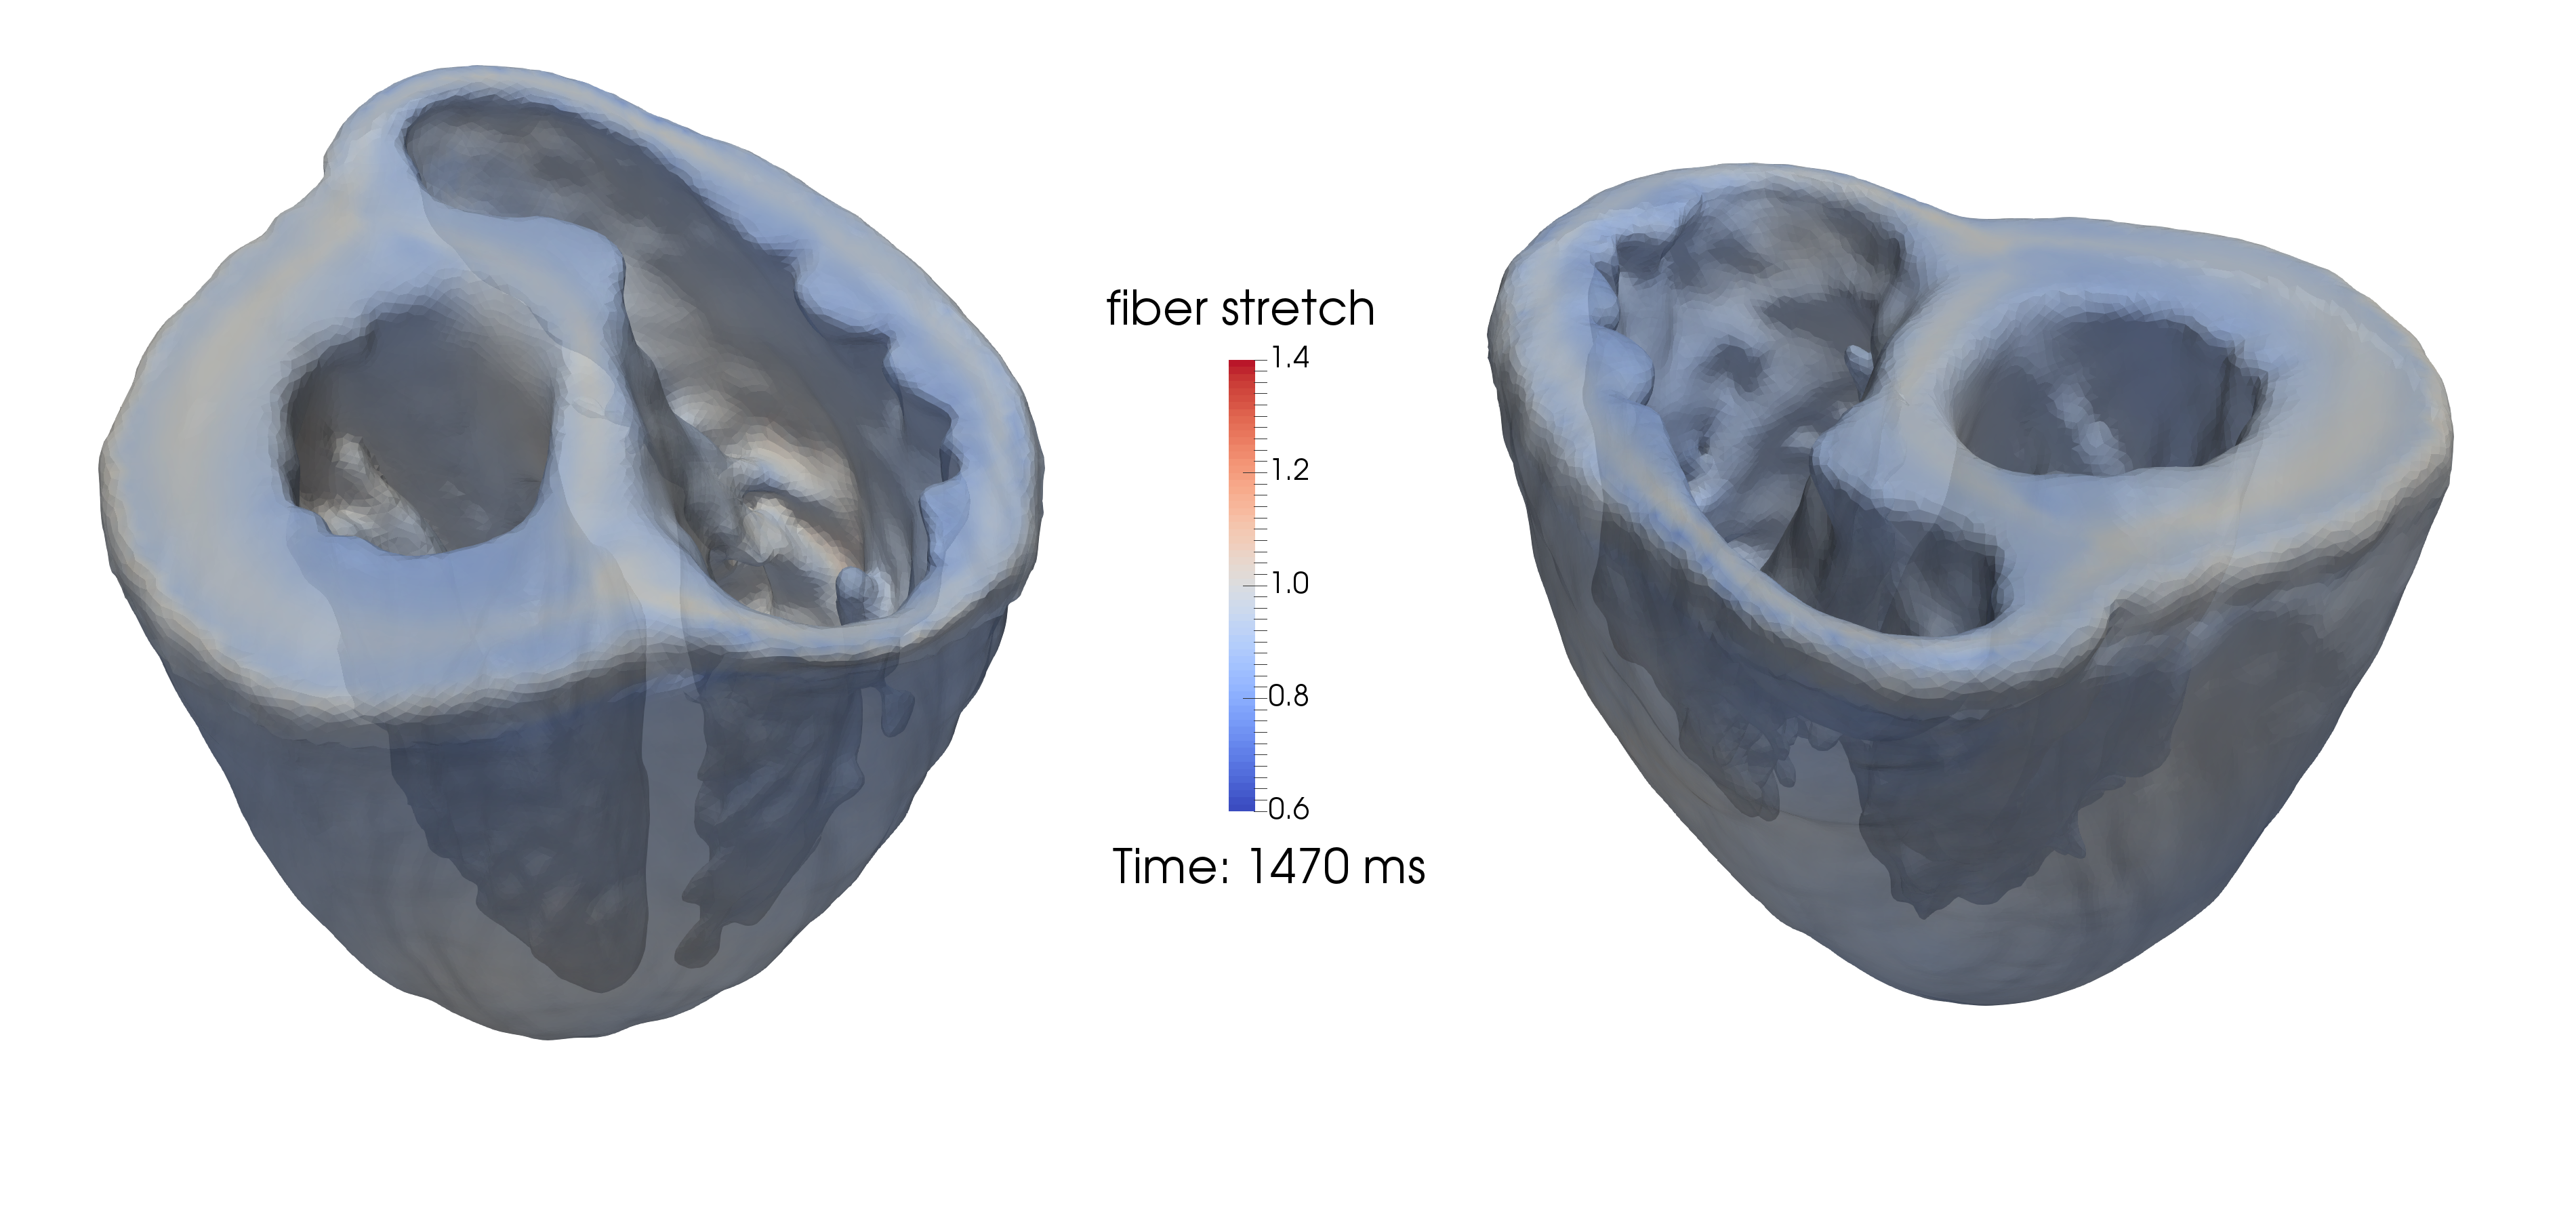
\includegraphics[scale=0.08]{media/4-cardioid/6-vid/d.png}
\label{fig:snaps4}}		
%
\caption{Deformed mesh from Cardioid simulation at different stages of cardiac cycle. Panels (a), (b), (c), and (d) correspond to the stages in the P-V loop denoted in~\figref{pv}.}
\label{fig:snaps}
\end{sidewaysfigure}

%%%%%%%%%%%%%%%%%%%%%%%%%%%%%%%%%%%%%%%%%%%%%%%
%%%%%%%%%%%%%%%%%%%%%%%%%%%%%%%%%%%%%%%%%%%%%%%
\section{Extension to Polyhedral Finite Elements}
\label{Polyhedral Finite Elements}

Efforts have been made to implement the mechanics described in this chapter into the polyhedral FEM code \textit{Celeris}. The details of the implementation will be discussed, followed by an expos\'{e} of cardiac verification problems using polyhedral finite elements.

\subsection{Implementation}

The same surface mesh used to produce the quadratic tetrahedral mesh for Cardioid is used to produce the polyhedral mesh in Celeris shown in \figref{compdof} and \figref{cel}. The fiber orientations, activation times, and surface tags are generated using Celeris and subsequently read into Celeris for use. The same Dirichlet boundary conditions applied in Cardioid are applied in Celeris using the same surface tags shown in \figref{supp3}. For simplicity, the ventricular pressure time histories from the Cardioid simulation are used directly for the imposition of ventricular boundary conditions in Celeris, rather than imposing volume constraints as described previously. Of course, in the future the volume constraint would be implemented as well so that the Celeris mechanics is completely independent of the Cardioid mechanics. The Cauchy pressure time histories $p_{LV}(t)$ and $p_{RV}(t)$ are enough to demonstrate the workflow using polyhedral FEM and highlighting the advantages of PEM over conventional FEM.

The remaining consideration of course is implementation of the material model, which is the focus of the remainder of this section.

\subsubsection{Material Model}
The Usyk material model is implemented within the Celeris framework. Rather than full incompressibility via a mixed displacement-pressure formulation, near-incompressibility is enforced via a penalty term in the strain energy for volumetric material response, together with an F-bar projection method. Regarding the penalty term, the strain energy is defined in the following manner, as is done by Usyk\textit{et al.}~\cite{usyk_2002}:
\begin{equation}
W = \frac{C}{2}\left(e^Q -1\right) + C_{compr} (J \cdot \ln J - J + 1) \\
\end{equation}
The parameter $C_{compr}$ is a penalty parameter, such that the volumetric response of the material is significantly stiffer than the deviatoric response. It was found that a value of $C_{compr} \geq 200  C$ gives good results compared to those when enforcing full incompressibility through a mixed pressure-displacement formulation, without significantly making the system poorly conditioned. Interestingly, the value of $C_{compr}$ provided by Usyk \textit{et al.} is actually not nearly large enough to produce results that are competitive with fully incompressible formulations. Near-incompressibility is then enforced by an F-bar projection method, in which the deformation gradient is modified such that the dilatation $det(\bm{F})$ at each integration point is replaced by a constant element-averaged value, as discussed in Doll~\textit{et al.}~\cite{doll_2000}.

\textbf{Passive stress}

The material model framework in Celeris currently accepts definitions in \textit{incremental form}, namely, the material model takes as input the material properties and other field parameters, the beginning step Cauchy stress $\overline{\bm{T}}$, beginning step state variables $\overline{\bm{s}}$, and strain rate $\bm{D}$, and produces as output an end step unrotated Cauchy stress $\tilde{\bm{T}}$, end step unrotated state variables $\tilde{\bm{s}}$, and end step tangent modulus $\frac{\partial \tilde{\bm{T}}}{\partial \bm{D}}$. Hyperelastic materials are generally defined as functions of the deformation gradient $\bm{F}$, though, not of the strain rate $\bm{D}$. As is done in \chapref{4} for the Mooney-Rivlin material, it is assumed that $\hat{\bm{U}} = \text{exp}(\bm{D}\Delta{t})$, which is approximated using its Taylor expansion as follows:
\begin{equation}
\hat{\bm{U}} = \bm{I} + \bm{D}\Delta{t} + \frac{1}{2}(\bm{D}\Delta{t})^2 + \frac{1}{6}(\bm{D}\Delta{t})^3
\end{equation}

The beginning step deformation gradient is stored as a state variable to accommodate the incremental material form. It is initialized as the identity tensor and updated within each call to the material model as $\tilde{\bm{F}} = \hat{\bm{U}}\bm{F}$. Field parameters at each integration point include: the fiber transformation matrix $\bm{Q}$, activation time $t_a$. Finally the material model also admits the fixed beat duration, as well as the beginning and end step times - quantities used in the calculation of active tension. The fiber transformation matrix $\bm{Q}$ and activation time $t_a$ are computed via Cardioid \textit{a priori} and are imported into Celeris at the integration points. It is important to distinguish between the \textit{transformation matrix} $\bm{Q}$ from the global to local fiber coordinate frames, and the \textit{rotation increment} $\hat{\bm{R}}$ that comprises the rotation portion of the incremental deformation gradient $\hat{\bm{F}}$.

Because of the additive stress decomposition, the passive and active stress are computed independently, and then added together at the end of the constitutive update. The passive material update proceeds as follows: the end step unrotated deformation gradient $\tilde{\bm{F}}$ is transformed into the local fiber coordinate system, the end step unrotated Cauchy stress is computed in the local fiber coordinate system, and finally it is transformed back into the global coordinate frame. Specifically, the computations proceed in the following manner (a ``prime'' corresponds to the tensor being expressed as a matrix in the local fiber coordinate frame):
\begin{align}
\tilde{\bm{F}}' &= \bm{Q}^T\tilde{\bm{F}}\bm{Q} \\
\bm{C}' &= \tilde{\bm{F}}'^T \tilde{\bm{F}}' \\
\bm{E}' &= \frac{1}{2}(\bm{C}' - \bm{I}) \\
J  &= \det{\tilde{\bm{F}}'}
\end{align}
\begin{equation}
\begin{aligned}
Q' &= b_{ff} E'^2_{ff} + b_{ss} E'^2_{ss} + b_{nn} E'^2_{nn} + \\
&\text{\ \ \ }b_{fs}\left(E'^2_{fs} + E'^2_{sf}\right) + b_{fn}\left(E'^2_{fn} + E'^2_{nf}\right) + b_{ns}\left(E'^2_{ns} + E'^2_{sn}\right)
\end{aligned}
\end{equation}
\begin{align}
N_{pq} &= 2 \left[\begin{array} {ccc} b_{ff} & b_{fs} & b_{fn} \\ b_{fs} & b_{ss} & b_{sn} \\ b_{fn} & b_{sn} & b_{nn} \end{array} \right] \\
\frac{\partial Q'}{\partial \bm{E}'} &= \bm{N} \circ \bm{E}' \\
\tilde{\bm{T}}' &= \frac{C}{2J}e^{Q'}\tilde{\bm{F}}'^T\frac{\partial{Q'}}{\partial{\bm{E}'}}\tilde{\bm{F}}' + (C_{comp}\text{ln}J)\bm{I} \\
\tilde{\bm{T}}_p &= \bm{Q} \tilde{\bm{T}}' \bm{Q}^T
\end{align}
Note the stress is computed by making use of the relationship $\bm{T} = J^{-1}\bm{F}\frac{\partial\bm{W}}{\partial \bm{E}} \bm{F}^T$. The \textit{Hadamard} or \textit{entrywise product} is employed in defining $\frac{\partial Q'}{\partial \bm{E}'}$, namely $\frac{\partial Q'}{\partial E'_{pq}} = N_{pq}E'_{pq}$ with no implied sum on the indices. The sequence of calculations shown result in an end step unrotated passive Cauchy stress $\tilde{\bm{T}}_p$.

The tangent modulus of the passive portion of stress is computed by way of successive use of the chain rule of differentiation:
\begin{align}
\frac{\partial (\tilde{T}_p)_{ij}}{\partial \tilde{T}'_{mn}} &= \frac{1}{2}\left[Q'_{im}Q'_{jn} + Q'_{in}Q'_{jm}\right] \\
A_{pq} &\equiv \frac{\partial Q'}{\partial E'_{pq}} \\
Z_{pqkl} &\equiv \frac{1}{2}N_{pq}\left[F_{kq}\delta_{pl} + F_{kp}\delta_{ql}\right] \text{ (no sum)}
\end{align}
\begin{equation}
\begin{aligned}
\frac{\partial \tilde{T}'_{ij}}{\partial \tilde{F}'_{kl}} &= \frac{C}{2} \Bigg[\frac{-1}{J}\tilde{F}'^{-1}_{lk}e^{Q'}A_{pq}\tilde{F}'_{ip}\tilde{F}'_{jq} + \frac{1}{2J} e^{Q'}(A_{ln}\tilde{F}'_{kn} + A_{ml}\tilde{F}'_{km})A_{pq}\tilde{F}'_{ip}\tilde{F}'_{jq} + \\
&\text{\ \ \ }\frac{1}{J}e^{Q'}Z_{pqkl}\tilde{F}'_{ip}\tilde{F}'_{jq} + \frac{1}{J}e^{Q'}(\delta_{ik}A_{pl}\tilde{F}'_{jp} + \delta_{jk}A_{lq}\tilde{F}'_{iq})\Bigg] + C_{comp}\delta_{ij}\tilde{F}'^{-1}_{lk}
\end{aligned}
\end{equation}
\begin{align}
\frac{\partial \tilde{F}'_{ij}}{\partial \tilde{F}_{mn}} &= Q'_{mi}Q'_{nj} \\
\frac{\partial \tilde{F}_{mn}}{\partial \hat{U}_{kl}} &= \frac{1}{2}\left[\delta_{ik}\overline{F}_{lj} + \delta_{il}\overline{F}_{kj}\right]
\end{align}
\begin{equation}
\begin{aligned}
\frac{\partial \hat{U}_{ij}}{\partial D_{kl}} = &\frac{1}{2}\left[\delta_{ik}\delta_{jl} + \frac{1}{2}\delta_{ik}D_{lj} + \frac{1}{2}D_{ik}\delta_{jl} + \frac{1}{6}\delta_{ik}D_{ln}D_{nj} + \frac{1}{6}D_{ik}D_{lj} + \frac{1}{6}D_{im}D_{mk}\delta_{jl}\right] + \\
&\frac{1}{2}\left[\delta_{il}\delta_{jk} + \frac{1}{2}\delta_{il}D_{kj} + \frac{1}{2}D_{il}\delta_{jk} + \frac{1}{6}\delta_{il}D_{kn}D_{nj} + \frac{1}{6}D_{il}D_{kj} + \frac{1}{6}D_{im}D_{ml}\delta_{jk}\right]
\end{aligned}
\end{equation}

Finally, the derivatives are combined to produce the tangent modulus:
\begin{equation}
\frac{\partial \tilde{\bm{T}}_p}{\partial (\bm{D}\Delta{t})} = \frac{\partial \tilde{\bm{T}}_p}{\partial \tilde{\bm{T}'}}\frac{\partial \tilde{\bm{T}'}}{\partial \tilde{\bm{F}'}}\frac{\partial \tilde{\bm{F}'}}{\partial \tilde{\bm{F}}}\frac{\partial \tilde{\bm{F}}}{\partial \hat{\bm{U}}}\frac{\partial \hat{\bm{U}}}{\partial (\bm{D}\Delta{t})}
\end{equation}

The passive material model has been implemented, and the computed stress and corresponding tangent modulus have been thoroughly verified against finite difference approximations for accurate and quickly converging solutions.

\textbf{Active stress}

%%%%%%%%%%%%%%%%%%%%%%%%%%%%%%%%%%%%%%%%%%%%%%%%%%
The Fortran code to compute the active stress $\tilde{\bm{T}}_a$ and corresponding tangent modulus $\frac{\partial \tilde{\bm{T}}_a}{\partial (\bm{D}\Delta{t})}$ is generated by the Cardioid tool \textit{Melodee}~\cite{melodee}, a new language for expressing systems of ODEs that generates optimized code for different platforms. Melodee was tested and verified to generate a working Fortran subroutine for the Lumens active stress model.

Finally, the passive and active stress, along with their tangent moduli, are combined in the following manner:
\begin{align}
\tilde{\bm{T}} &= \tilde{\bm{T}}_p + \tilde{\bm{T}}_a \\
\frac{\partial \tilde{\bm{T}}}{\partial (\bm{D}\Delta{t})} &= \frac{\partial \tilde{\bm{T}}_p}{\partial (\bm{D}\Delta{t})}+ \frac{\partial \tilde{\bm{T}}_a}{\partial (\bm{D}\Delta{t})}
\end{align}

Lastly, outside of the constitutive update routine, the end step Cauchy stress and tangent modulus are forward rotated as discussed in \chapref{4}. Additionally, the state variable $\bm{F}$ is forward rotated simply via $\bm{F} =\hat{\bm{R}}\tilde{\bm{F}}$.

%%%%%%%%%%%%%%%%%%%%%%%%%%%%%%%%%%%%%%%%%%%%%%%%%%%%%%%%
%%%%%%%%%%%%%%%%%%%%%%%%%%%%%%%%%%%%%%%%%%%%%%%%%%%%%%%%

\subsection{Verification}

All compoenents required to perform a complete cardiac simulation have been implemented. Prior to running a complete cardiac simulation, though, the polyhedral workflow was tested for a suite of verification problems. Six verification problems were identified: three from Gurev \textit{et al.}~\cite{gurev_2015} and three from Land \textit{et al.}~\cite{land_2015}. The specifics of those problems can be found in the those papers. See \figref{beams} and \figref{ventricles} for the nomenclature used to identify the problems, as well as the type of mechanics being tested for each one.

\begin{figure}[ht]
\centering
\subfigure[]{%
		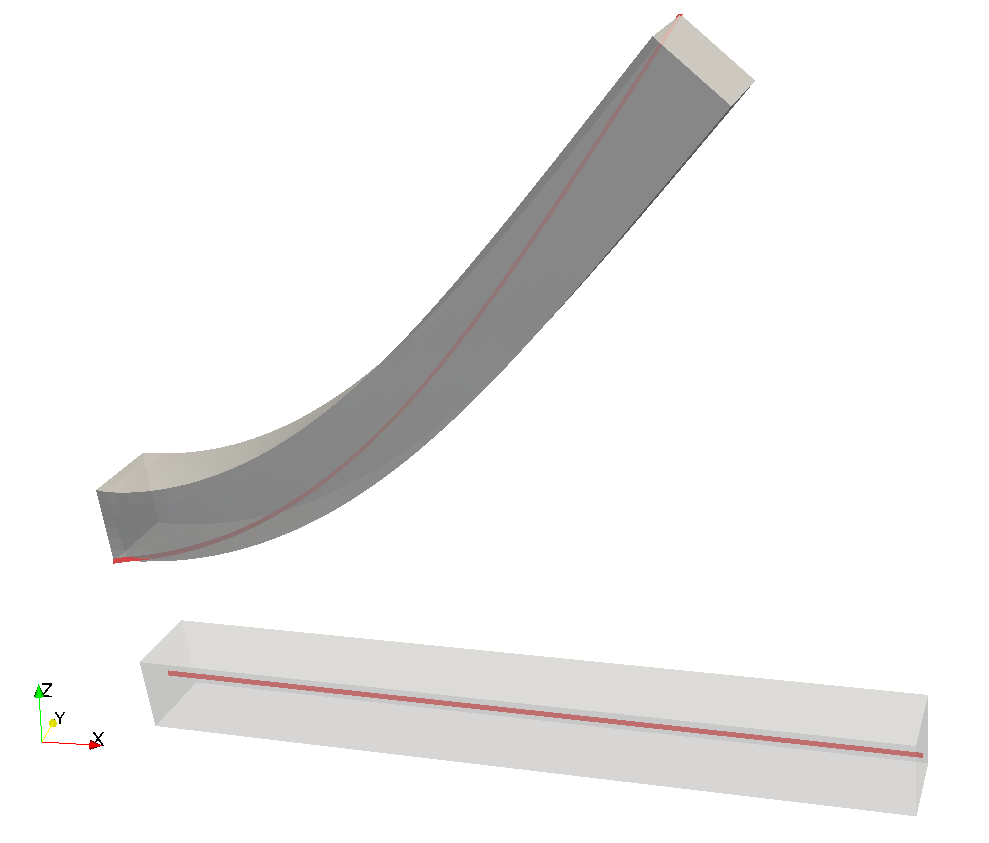
\includegraphics[scale=0.18]{media/5-verif/1-gurev2/gurev2.png}
\label{fig:beams1}}		
\subfigure[]{%
		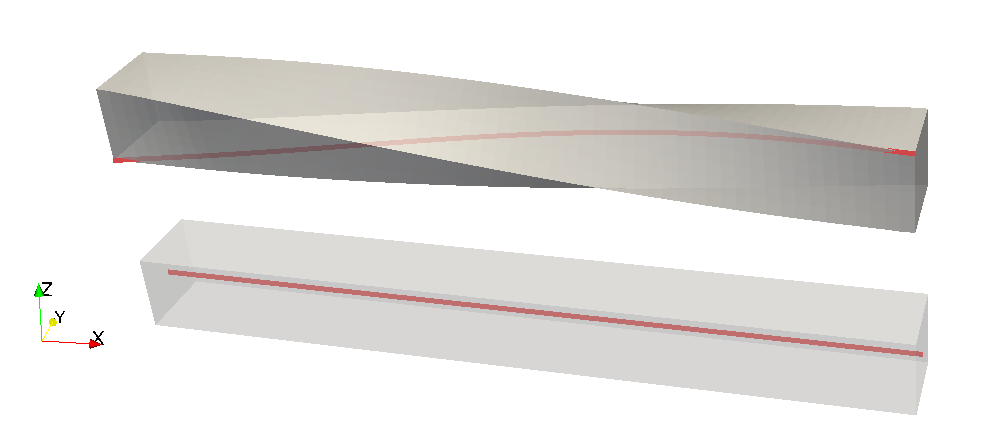
\includegraphics[scale=0.18]{media/5-verif/2-gurev3/gurev3.png}
\label{fig:beams2}}		
\subfigure[]{%
		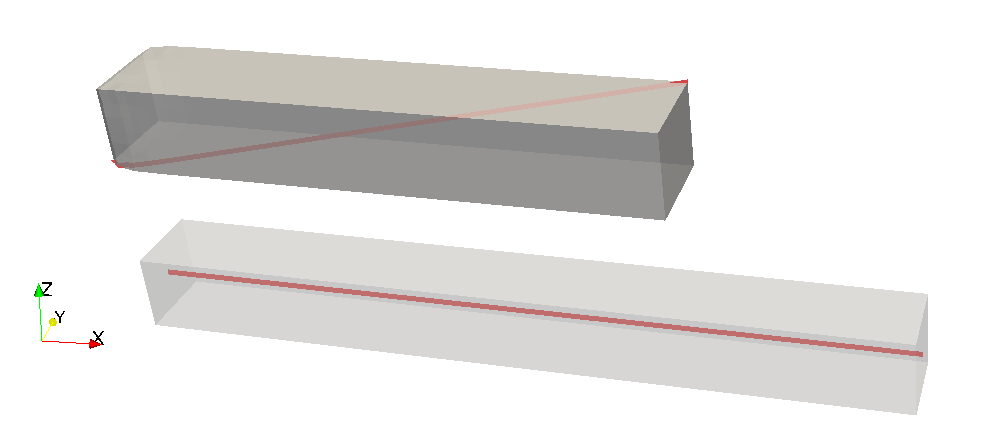
\includegraphics[scale=0.18]{media/5-verif/3-gurev4/gurev4.png}
\label{fig:beams3}}		
\subfigure[]{%
		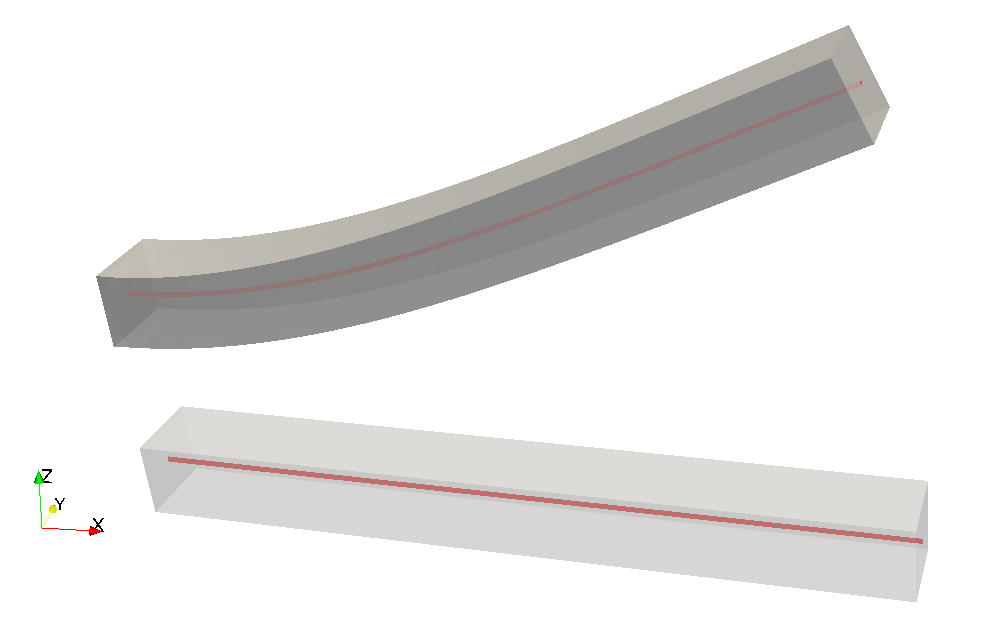
\includegraphics[scale=0.18]{media/5-verif/4-land1/land1.png}
\label{fig:beams4}}		
%
\caption{Undeformed (bottom) and deformed (top) configurations for cantilever beam verification problems: (a) Gurev P2: bending, (b) Gurev P3: torsion, c) Gurev P4: active contraction, and (d) Land P1: bending. The red curve denotes the curve over which displacements and positions are recorded and compared.}
\label{fig:beams}
\end{figure}

\begin{figure}[ht]
\centering
\subfigure[]{%
		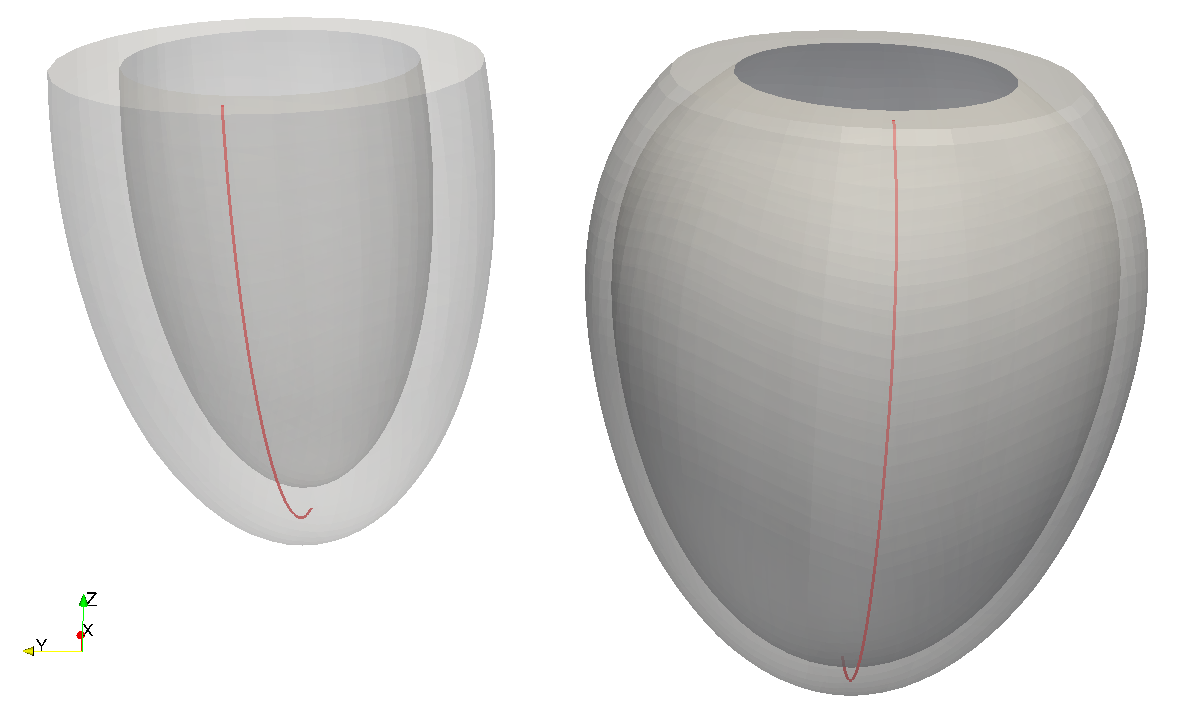
\includegraphics[scale=0.18]{media/5-verif/5-land2/land2-1.png}
\label{fig:ventricles1}}		
\subfigure[]{%
		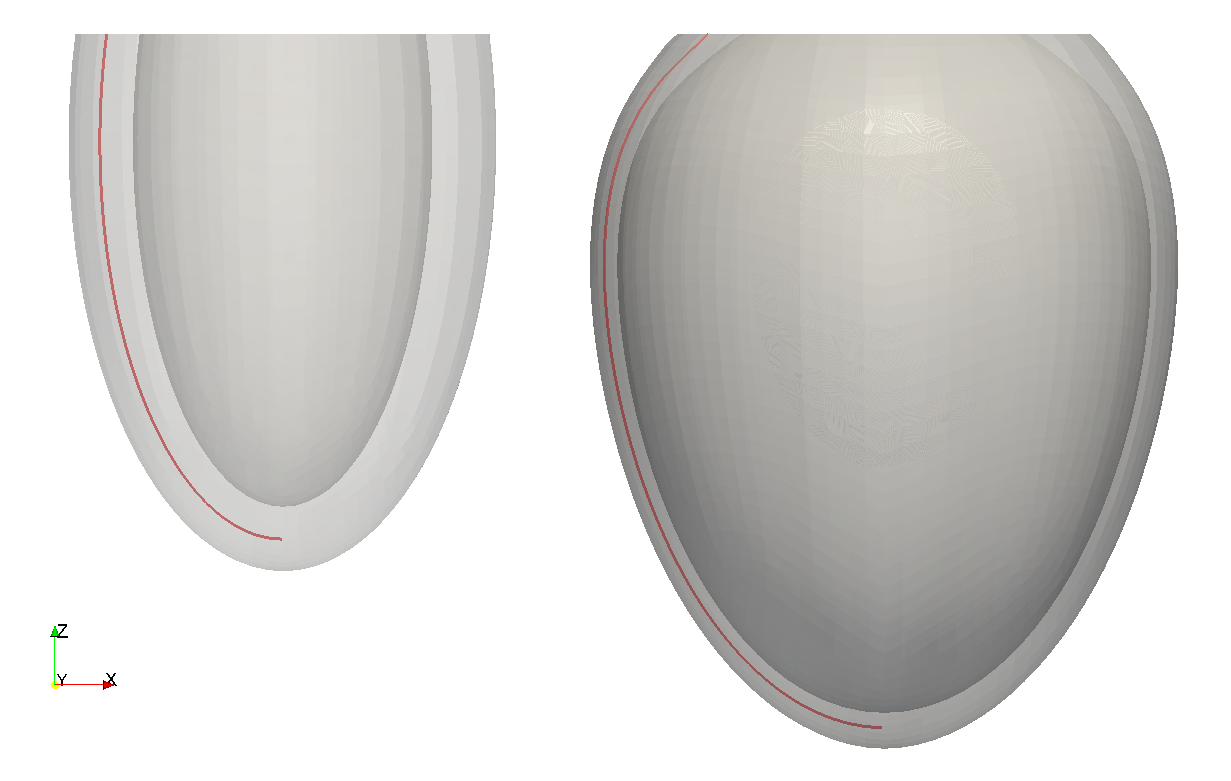
\includegraphics[scale=0.18]{media/5-verif/5-land2/land2-2.png}
\label{fig:ventricles2}}		
\subfigure[]{%
		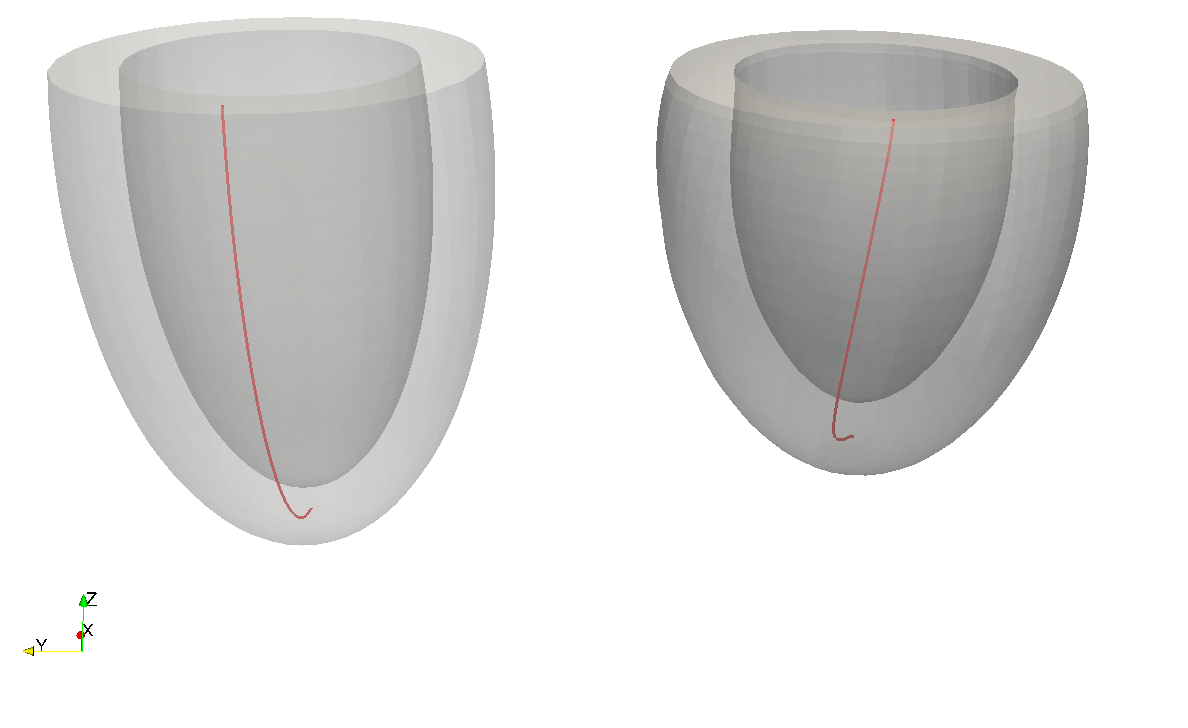
\includegraphics[scale=0.18]{media/5-verif/6-land3/land3-1.png}
\label{fig:ventricles3}}		
\subfigure[]{%
		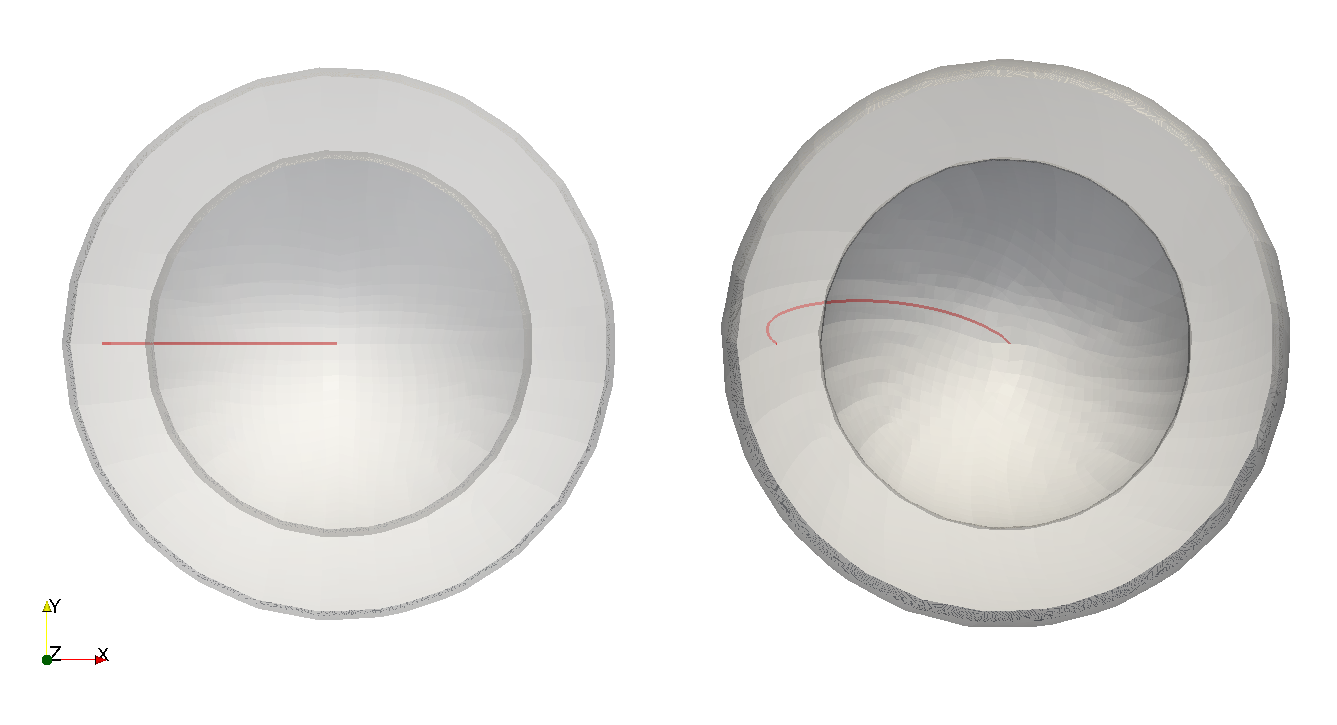
\includegraphics[scale=0.16]{media/5-verif/6-land3/land3-2.png}
\label{fig:ventricles4}}		
%
\caption{Undeformed (left) and deformed (right) configurations for single ventricle verification problems: (a,b) Land P2: inflation, and (c,d) Land P3: inflation and active contraction. The red curve denotes the curve over which displacements and positions are recorded and compared.}
\label{fig:ventricles}
\end{figure}

Figures \ref*{fig:gurev2}-\ref*{fig:land3.2} show the results for the six verification problems, mimicking the format used in the papers from which they came. The results are presented using Cardioid, Celeris, and an in-house finite element code \textit{Imitor}. The implementation considerations are nearly identical for Imitor and Celeris. Thus, differences in results can be distinguished based on the finite element formulation vs. the implementation of material model, near incompressibility, and the like.

As the figures show, the polyhedral code Celeris performs very well for the cantilever beam verification problems involving bending, twist, and active contraction. The deformed meshes nearly identically match those from the conventional FEM codes. For those problems, hexahedral elements are employed for the conventional FEM codes, and cuboidal PEM elements are used in Celeris. Namely, the element shapes are the same, while the element formulations differ.

Interestingly, the near-incompressible approach appears to be slightly too stiff in bending, but slightly too compliant in purely volumetric deformations based on the results exhibited using Imitor. The over-stiffness in bending is evidenced in Gurev P2, Land P1, and Land P2, whereas the over-compliance in volumetric deformation is evidenced in Gurev P4 and Land P3. Overall though, these results provide confidence that the codes are working correctly. 

Running Celeris for the single ventricular problems Land P2 and Land P3 hinges on some fixes in the infrastructure of that code, unrelated to the scope of this project. It is the hope that once these fixes are made, the suite of verification problems can be completed for all three codes referenced. A comparison of the number of degrees of freedom for Land P1 is provided (\figref{land1-3}), but it is not particularly interesting because the meshes are already quite coarse, and automated linear hex meshing for a simple cantilever beam geometry is easily achievable. It is the hope that for Land P2 and Land P3, accurate results can be achieved using Celeris with a significant reduction in the number of DOF, as explained in \chapref{3}.

Up to this point, the mechanics have been verified to be implemented correctly in Imitor and Celeris, and cuboidal polyhedral elements are performing well for the cantilever beam problems. Completing the verification process would involve running Land P2 and Land P3 in Celeris, as well as potentially running the cantilever beam problems again in Celeris with non-cuboidal polyhedral elements - after which point Celeris would be ready to perform the same cardiac simulations presented using Cardioid.

\begin{figure}[ht]
\centering
\subfigure[]{%
		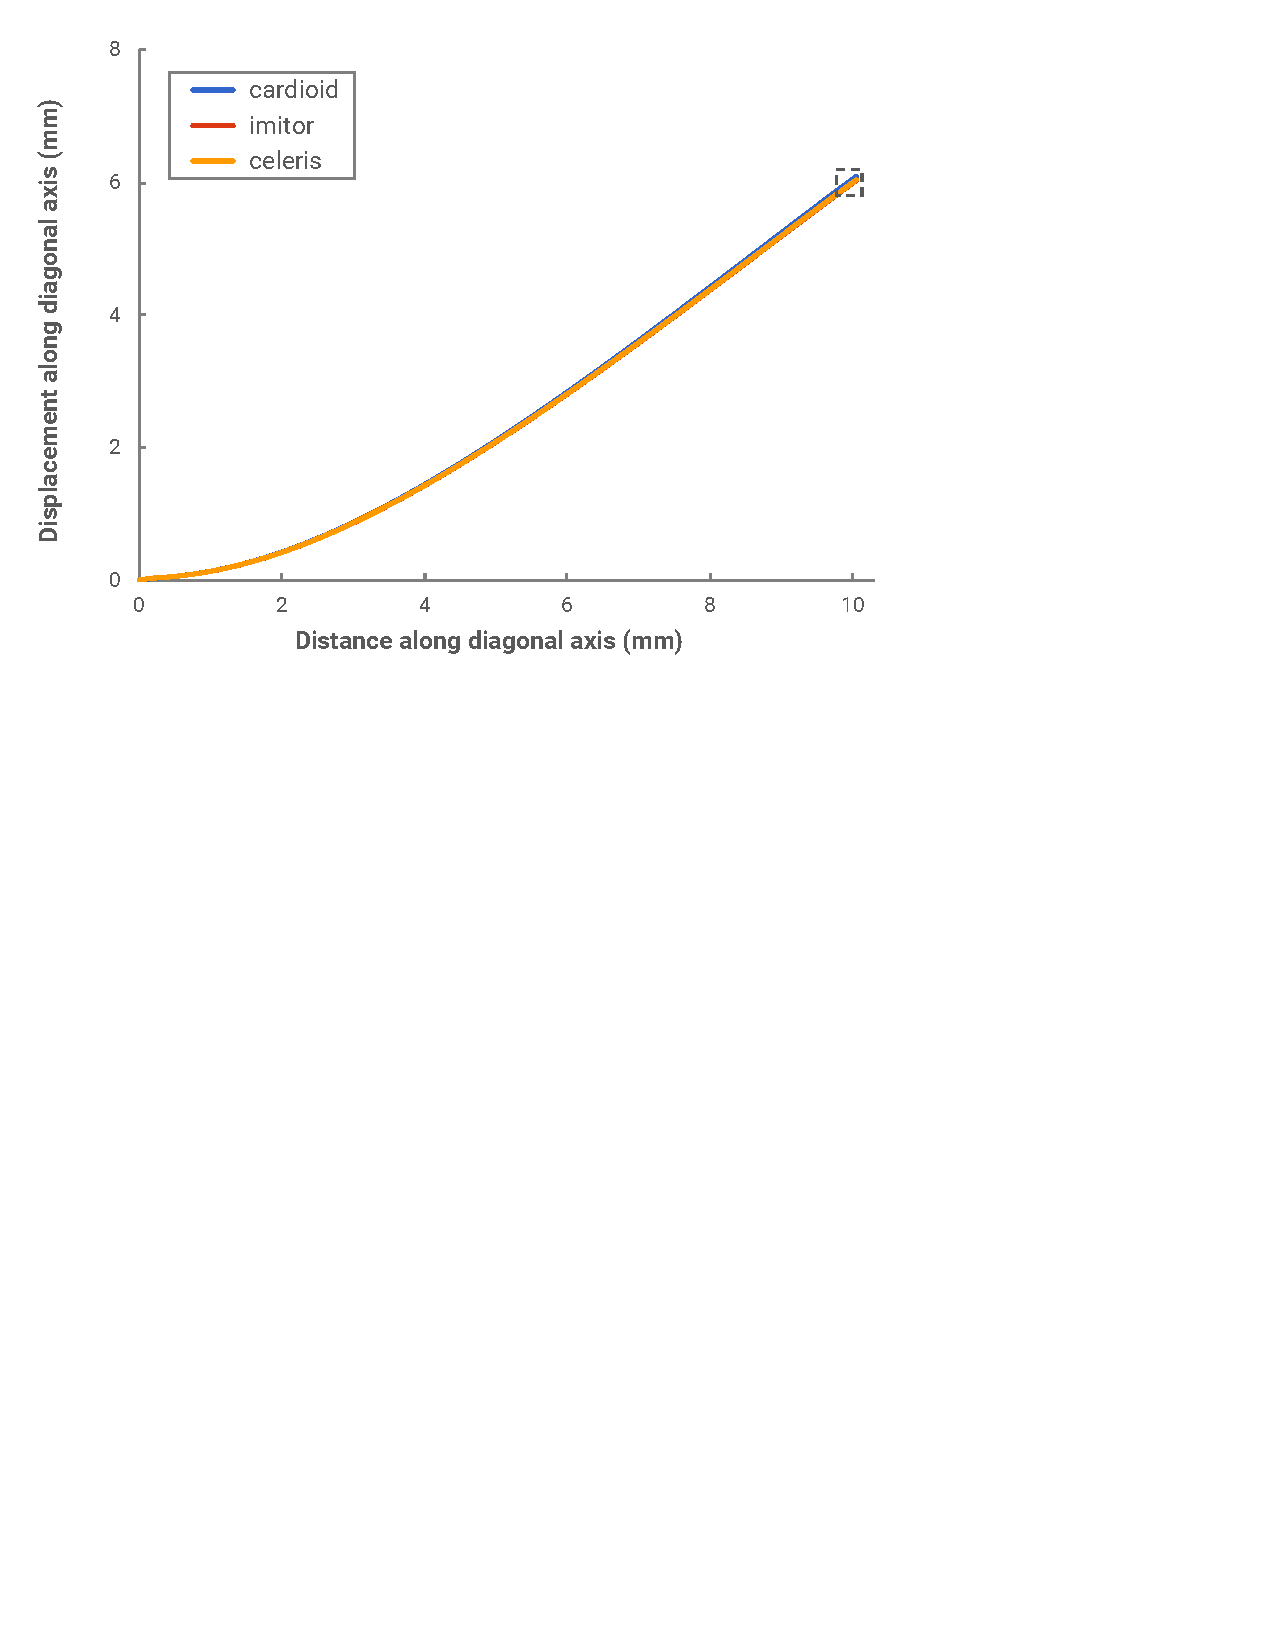
\includegraphics[scale=0.46]{media/5-verif/1-gurev2/gurev2-1.pdf}
\label{fig:gurev2-1}}		
\subfigure[]{%
		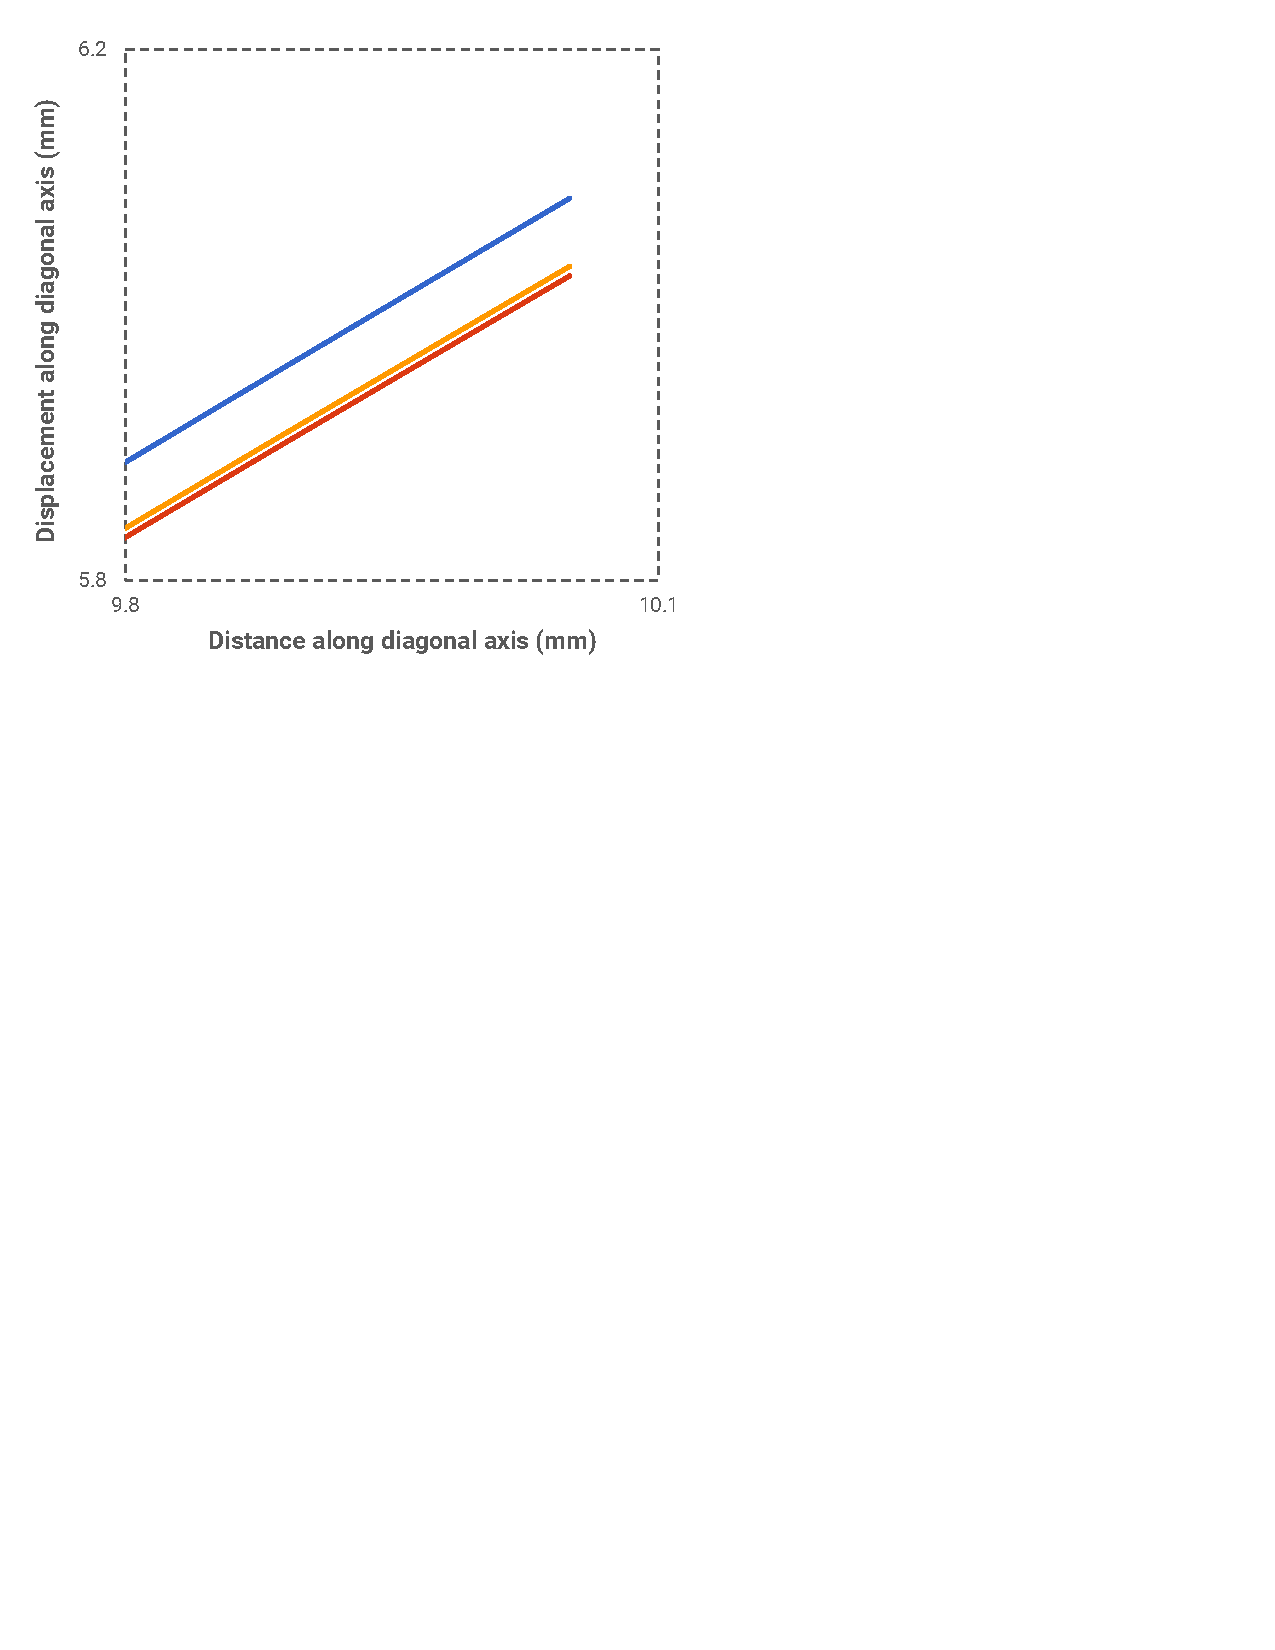
\includegraphics[scale=0.46]{media/5-verif/1-gurev2/gurev2-2.pdf}
\label{fig:gurev2-2}}		
%
\caption{Results for Gurev P2 verification problem: (a) Displacement magnitude along diagonal axis, with (b) details for the free end of the beam}
\label{fig:gurev2}
\end{figure}

\begin{figure}[ht!]
\centering
\subfigure[]{%
		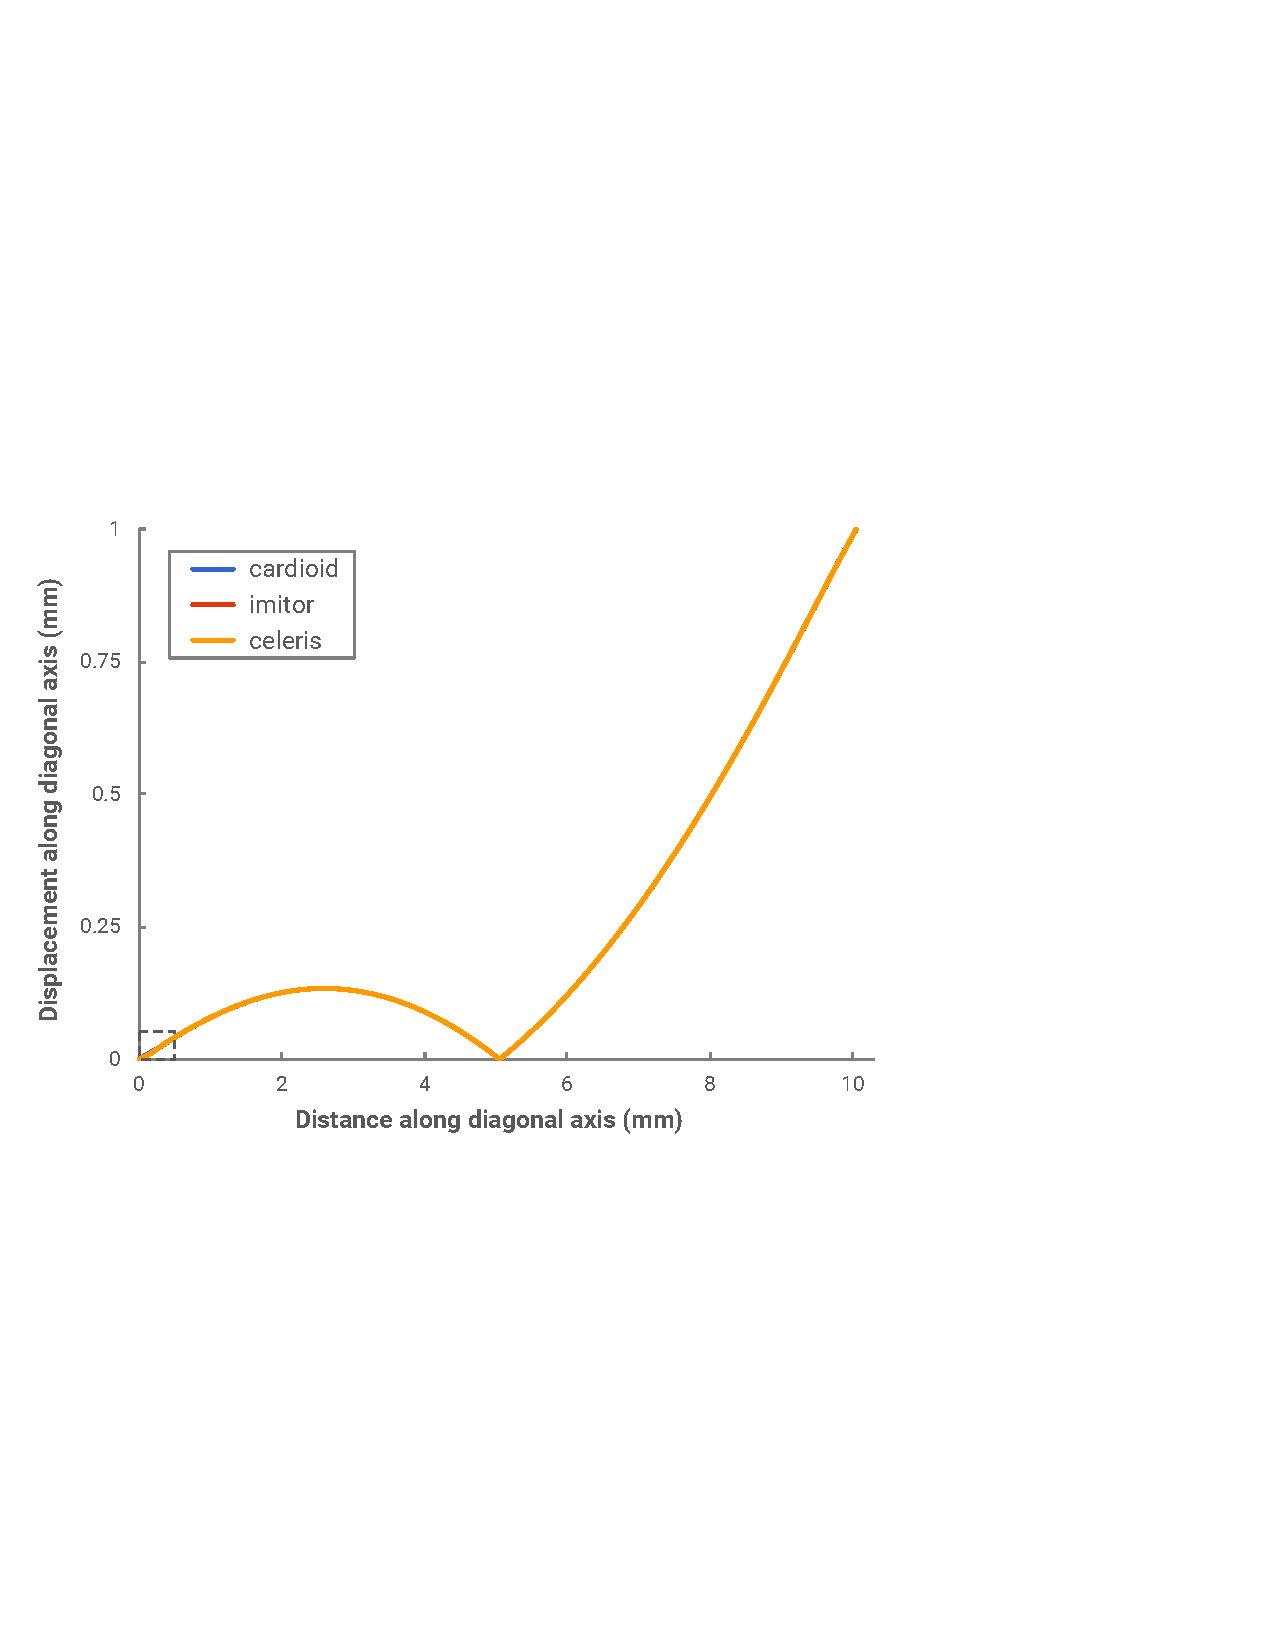
\includegraphics[scale=0.46]{media/5-verif/2-gurev3/gurev3-1.pdf}
\label{fig:gurev3-1}}		
\subfigure[]{%
		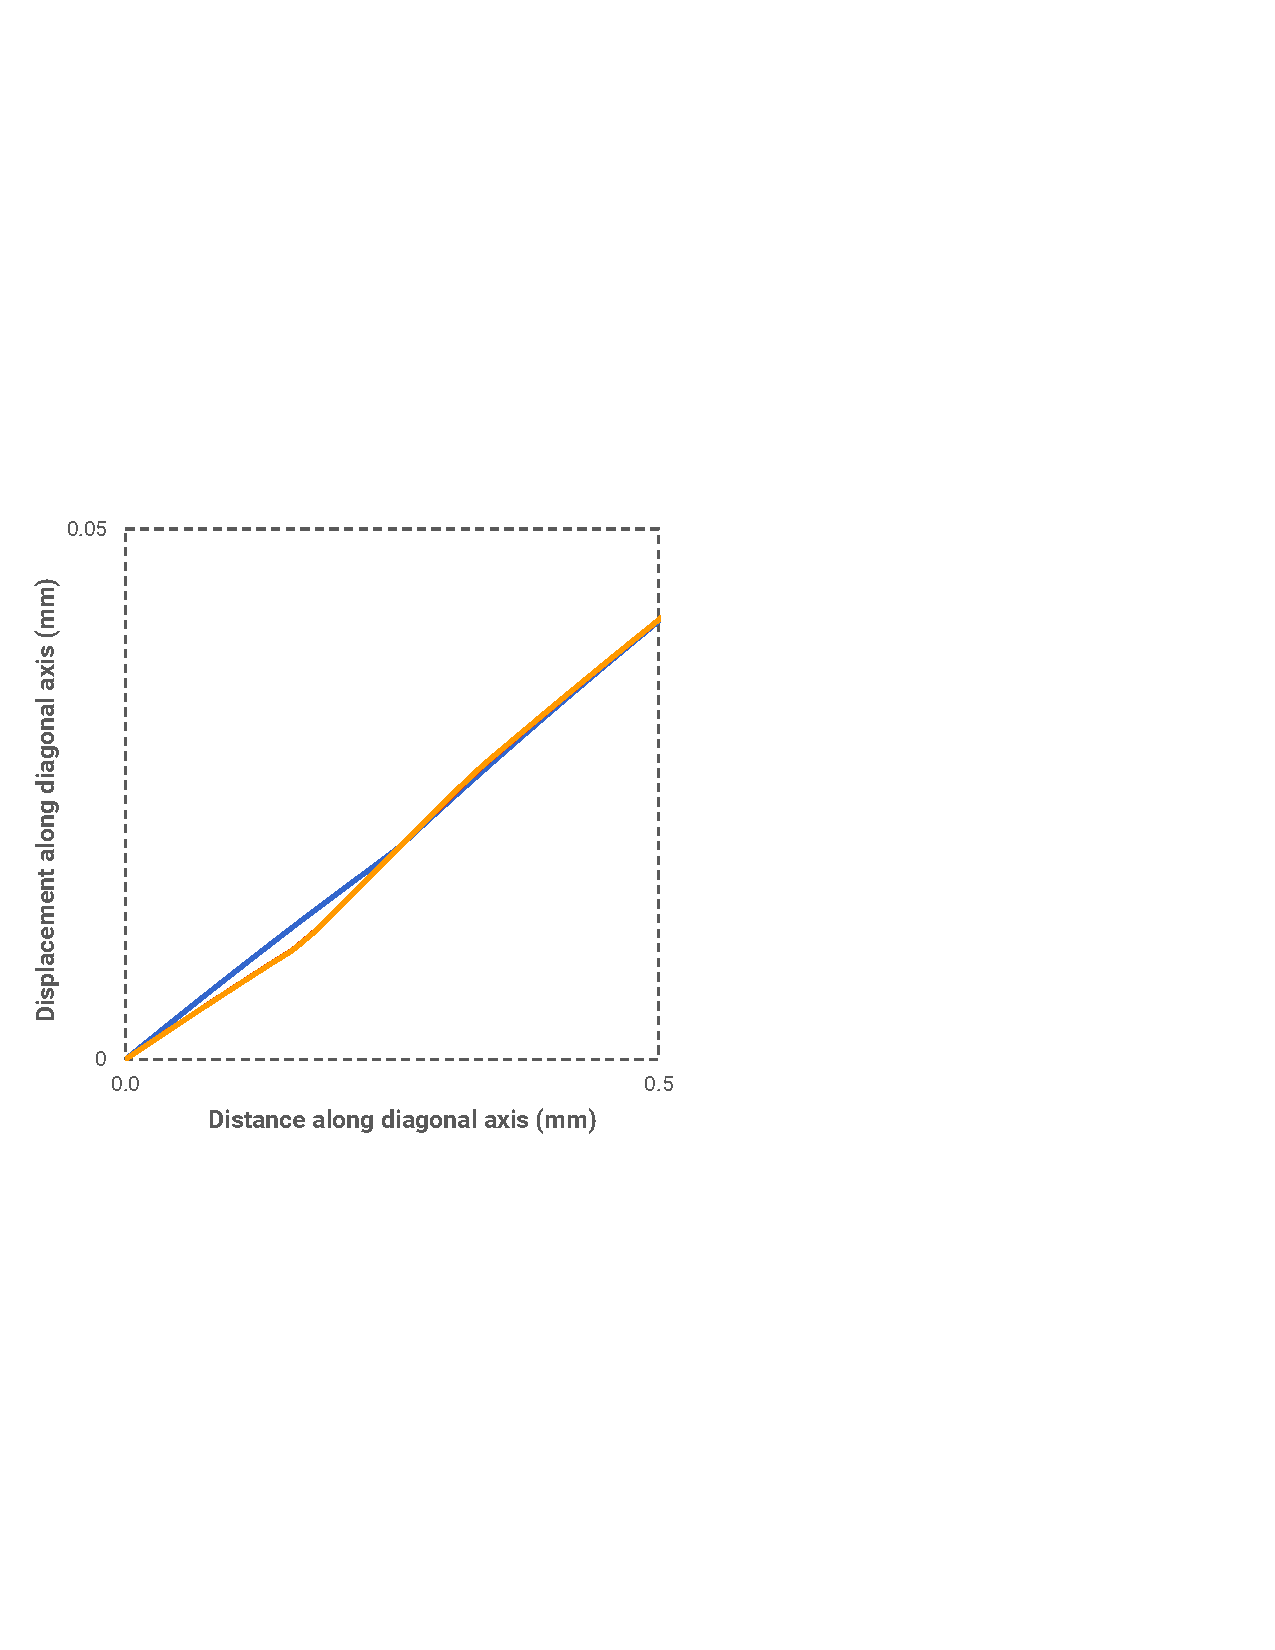
\includegraphics[scale=0.46]{media/5-verif/2-gurev3/gurev3-2.pdf}
\label{fig:gure3-2}}		
%
\caption{Results for Gurev P3 verification problem: (a) Displacement magnitude along diagonal axis, with (b) details for the fixed end of the beam. The results for imitor and Celeris are indistinguishable in these plots.}
\label{fig:gurev3}
\end{figure}

\begin{figure}[ht!]
\centering
\subfigure[]{%
		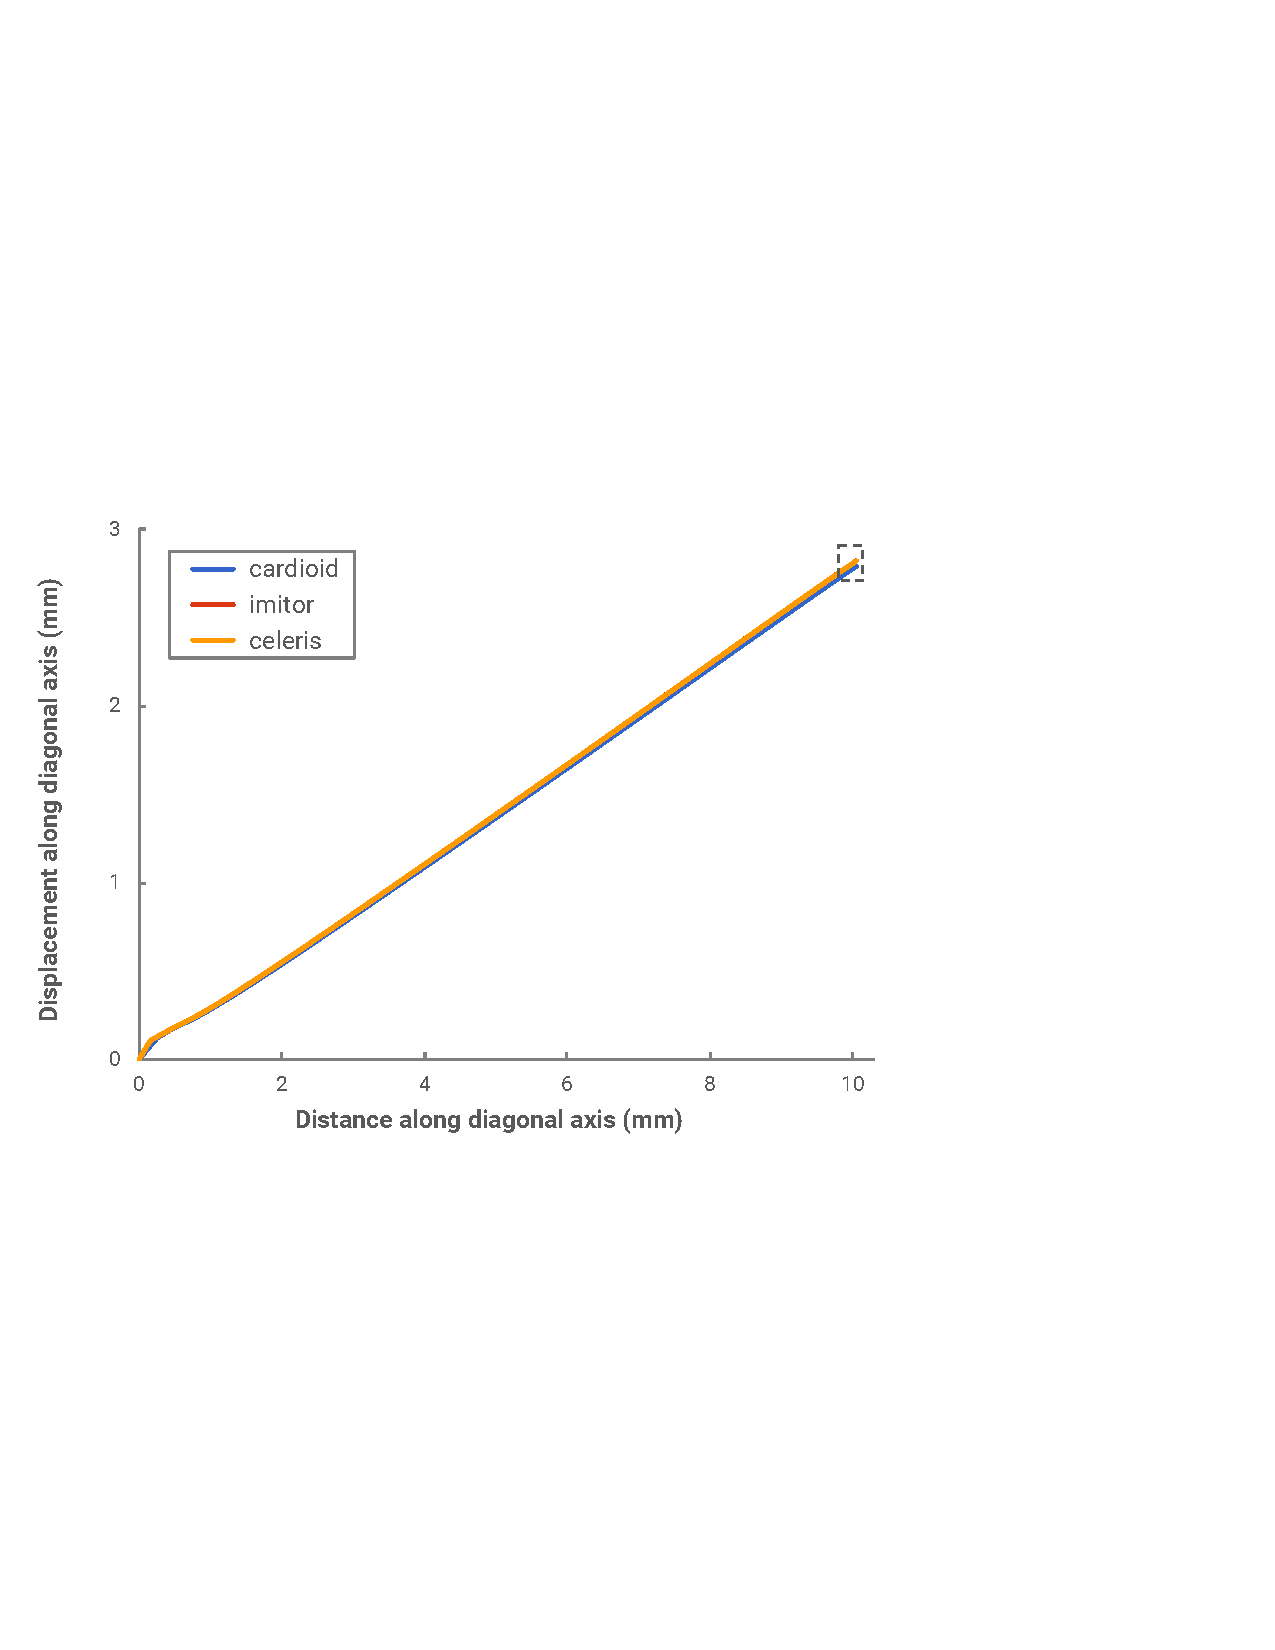
\includegraphics[scale=0.46]{media/5-verif/3-gurev4/gurev4-1.pdf}
\label{fig:gurev4-1}}		
\subfigure[]{%
		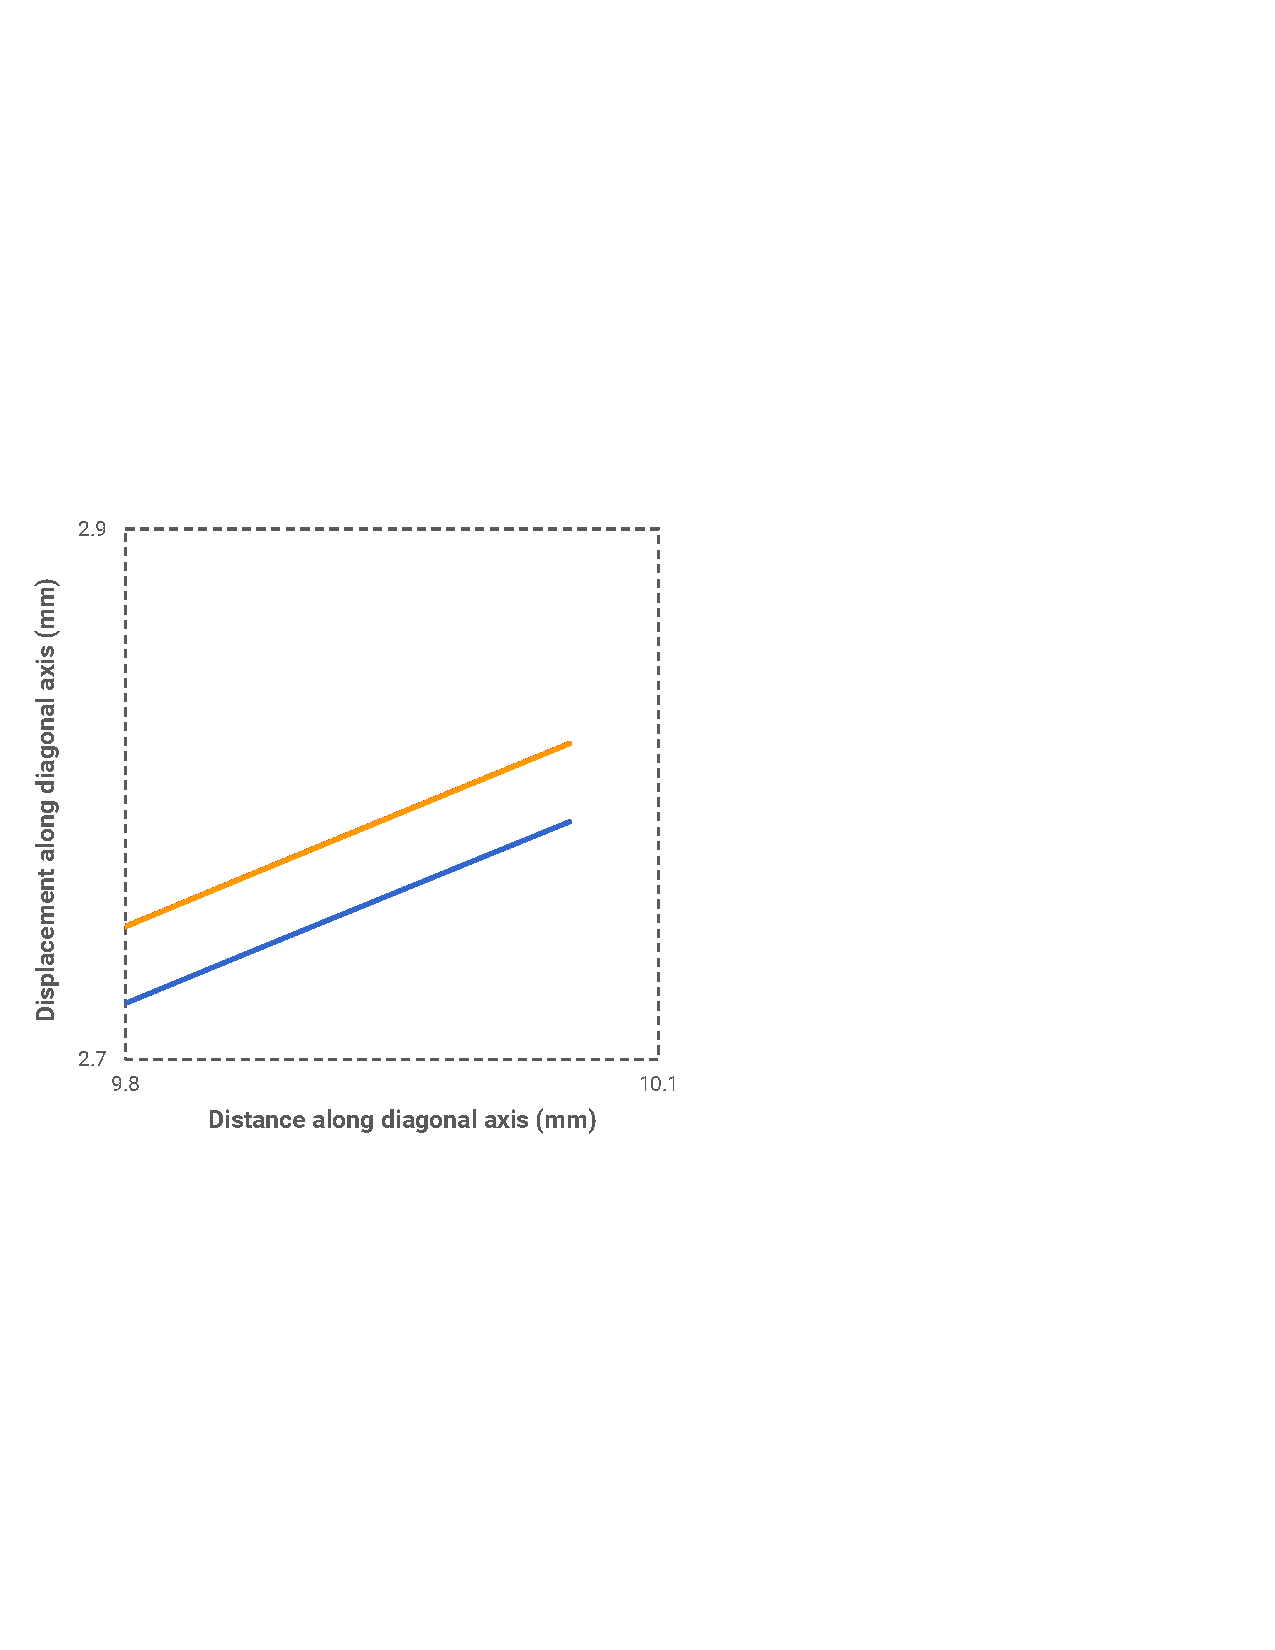
\includegraphics[scale=0.46]{media/5-verif/3-gurev4/gurev4-2.pdf}
\label{fig:gurev4-2}}		
%
\caption{Results for Gurev P4 verification problem: (a) Displacement magnitude along diagonal axis, with (b) details for the free end of the beam. The results for imitor and Celeris are indistinguishable in these plots.}
\label{fig:gurev4}
\end{figure}

\begin{figure}[ht!]
\centering
\subfigure[]{%
		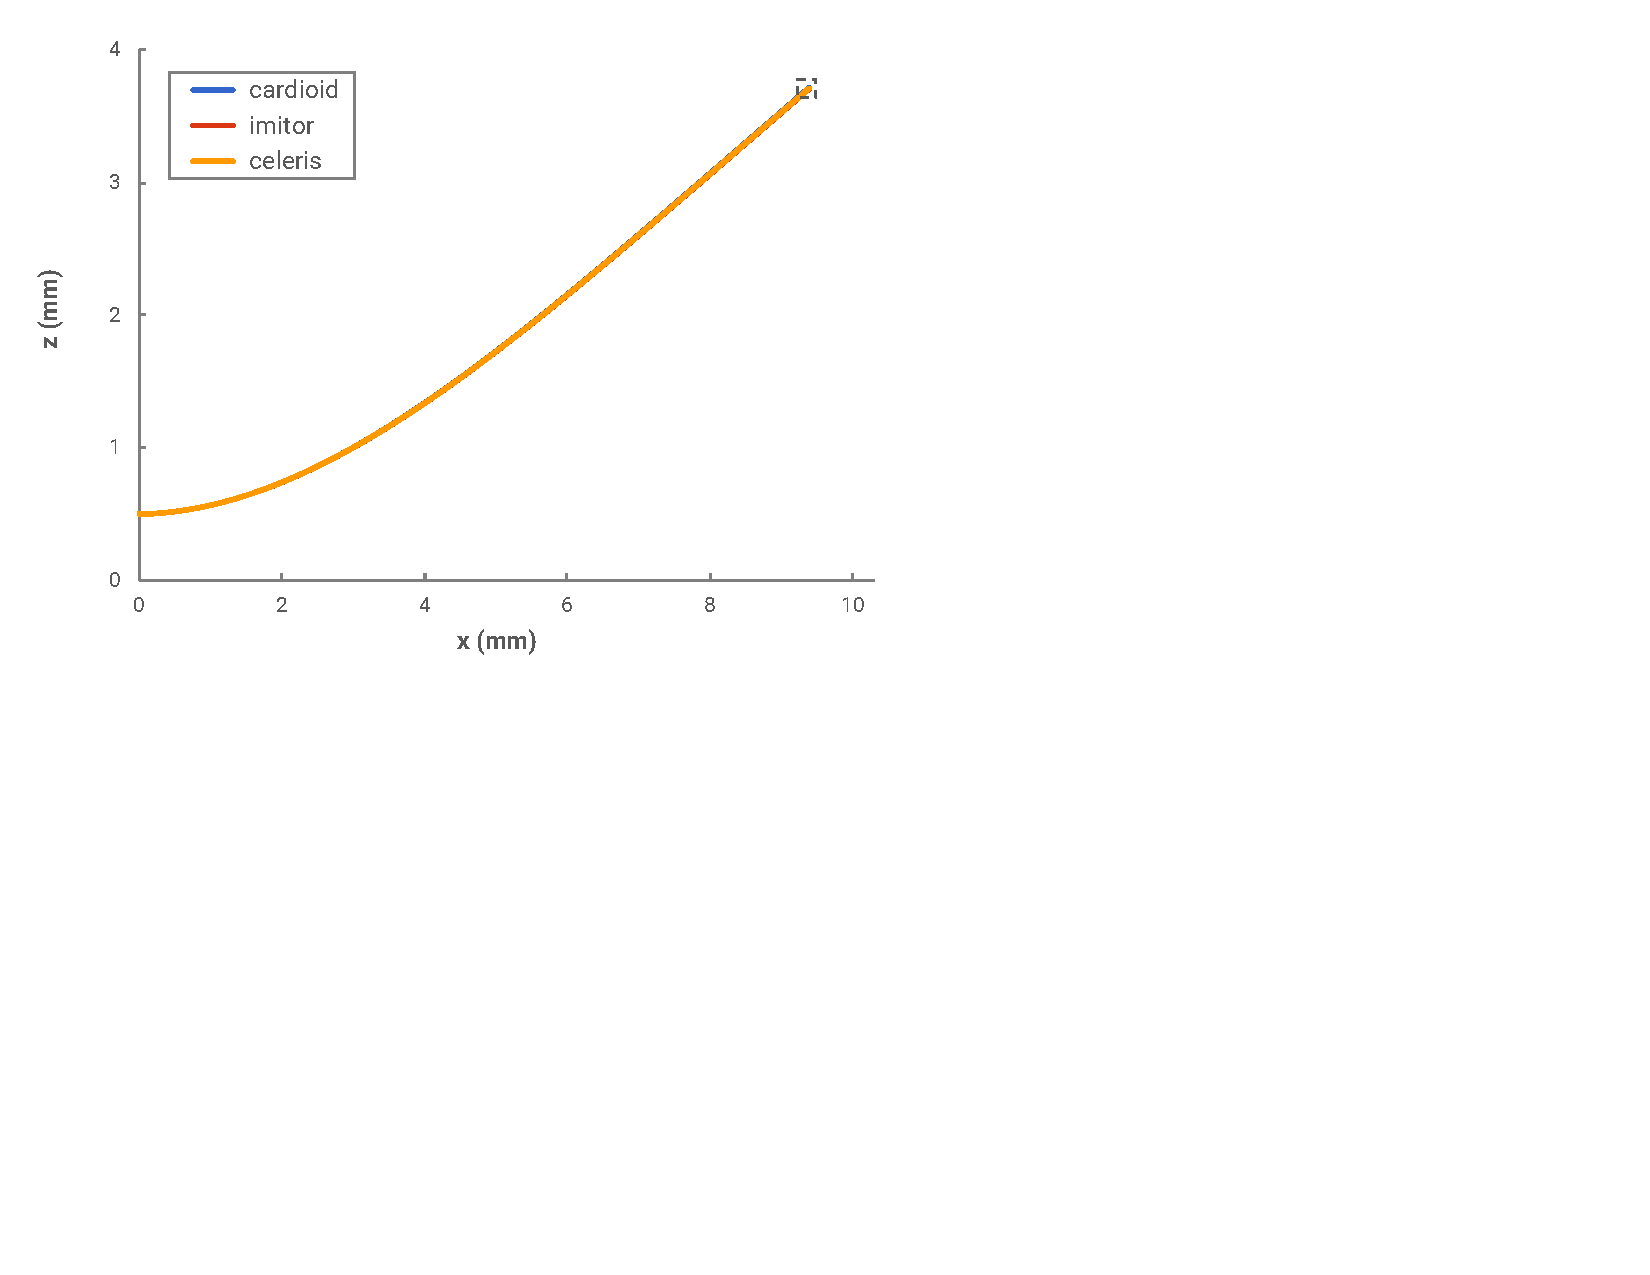
\includegraphics[scale=0.46]{media/5-verif/4-land1/land1-1.pdf}
\label{fig:land1-1}}		
\subfigure[]{%
		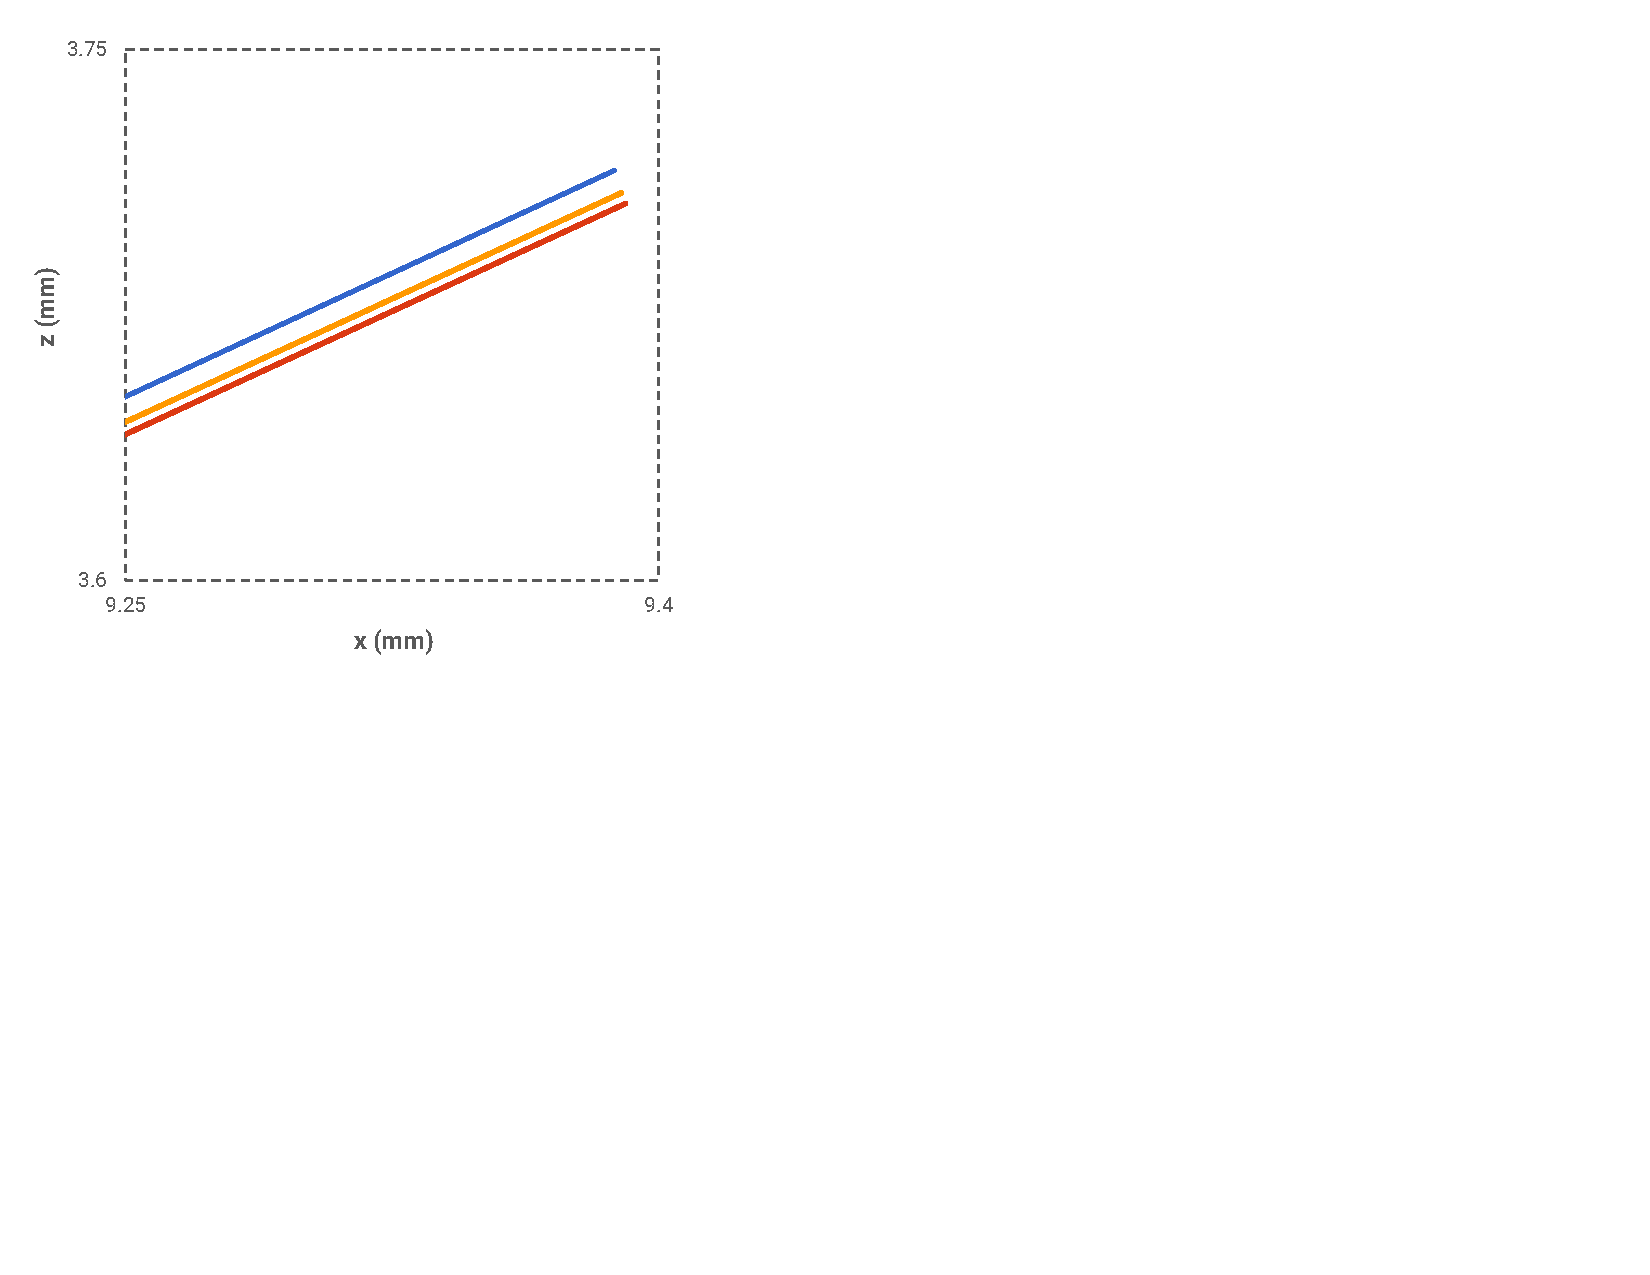
\includegraphics[scale=0.46]{media/5-verif/4-land1/land1-2.pdf}
\label{fig:land1-2}}	
\subfigure[]{%
		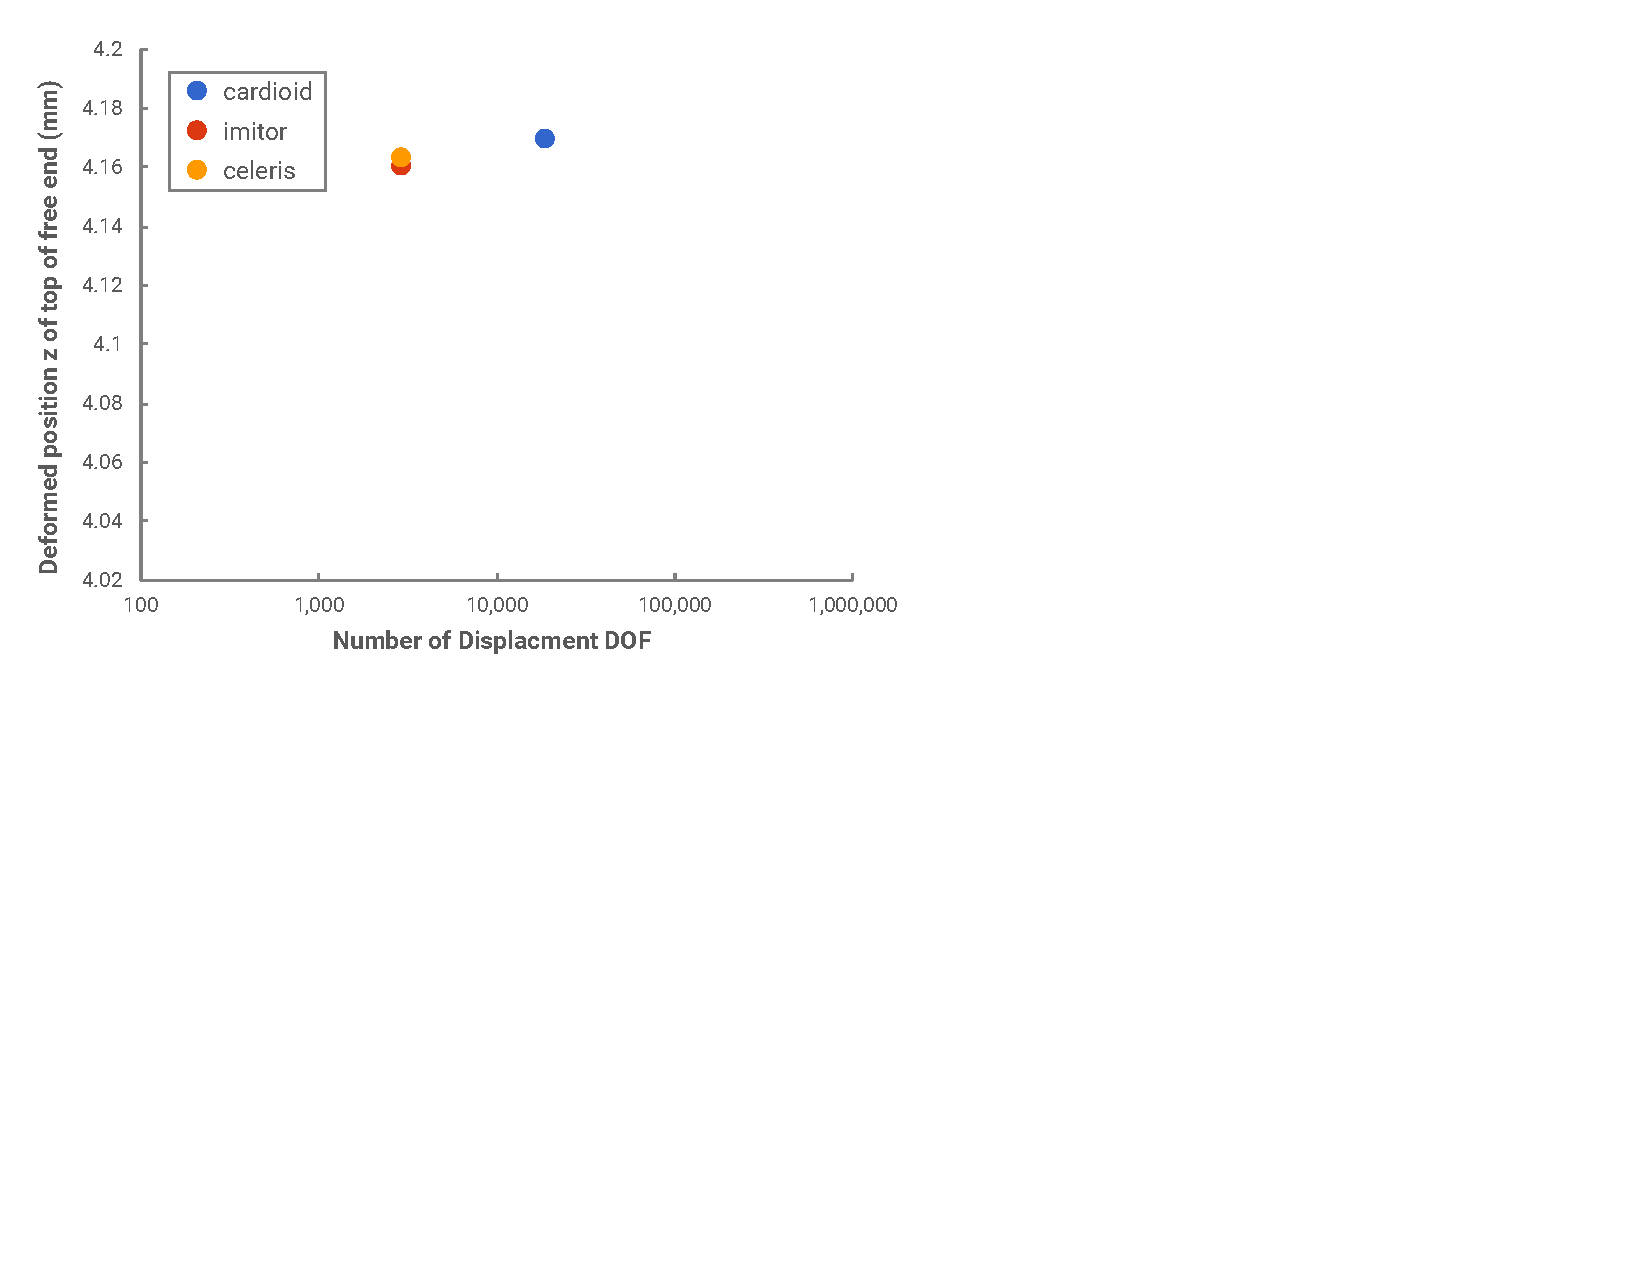
\includegraphics[scale=0.46]{media/5-verif/4-land1/land1-3.pdf}
\label{fig:land1-3}}			
%
\caption{Results for Land P1 verification problem: (a) Deformed position of midline, with (b) details for the free end of the beam. Panel (c) shows the deformed position of the point $\bm{X} = (10, 0.5, 1)$ for each of the simulation codes.}
\label{fig:land1}
\end{figure}


\begin{figure}[ht!]
\centering
\subfigure[]{%
		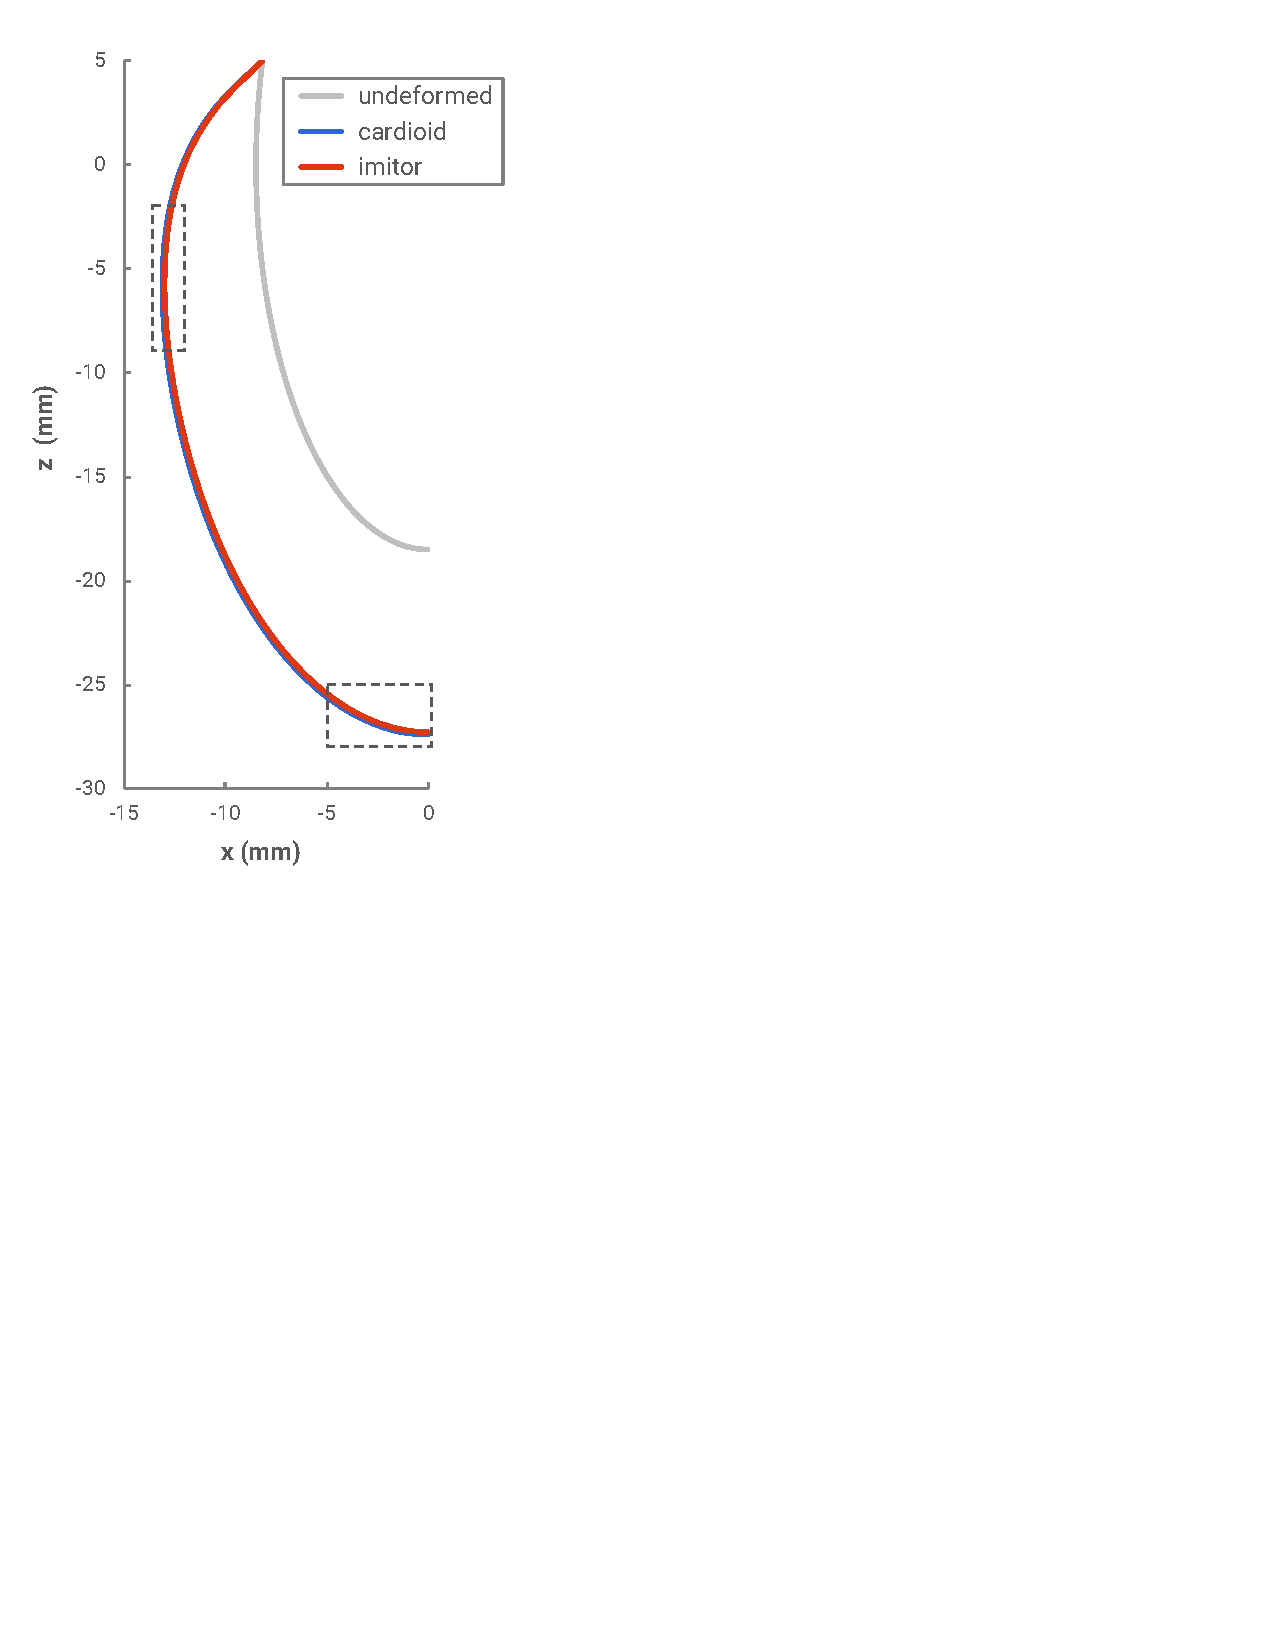
\includegraphics[scale=0.46]{media/5-verif/5-land2/land2-1.pdf}
\label{fig:land2-1}}		
\subfigure[]{%
		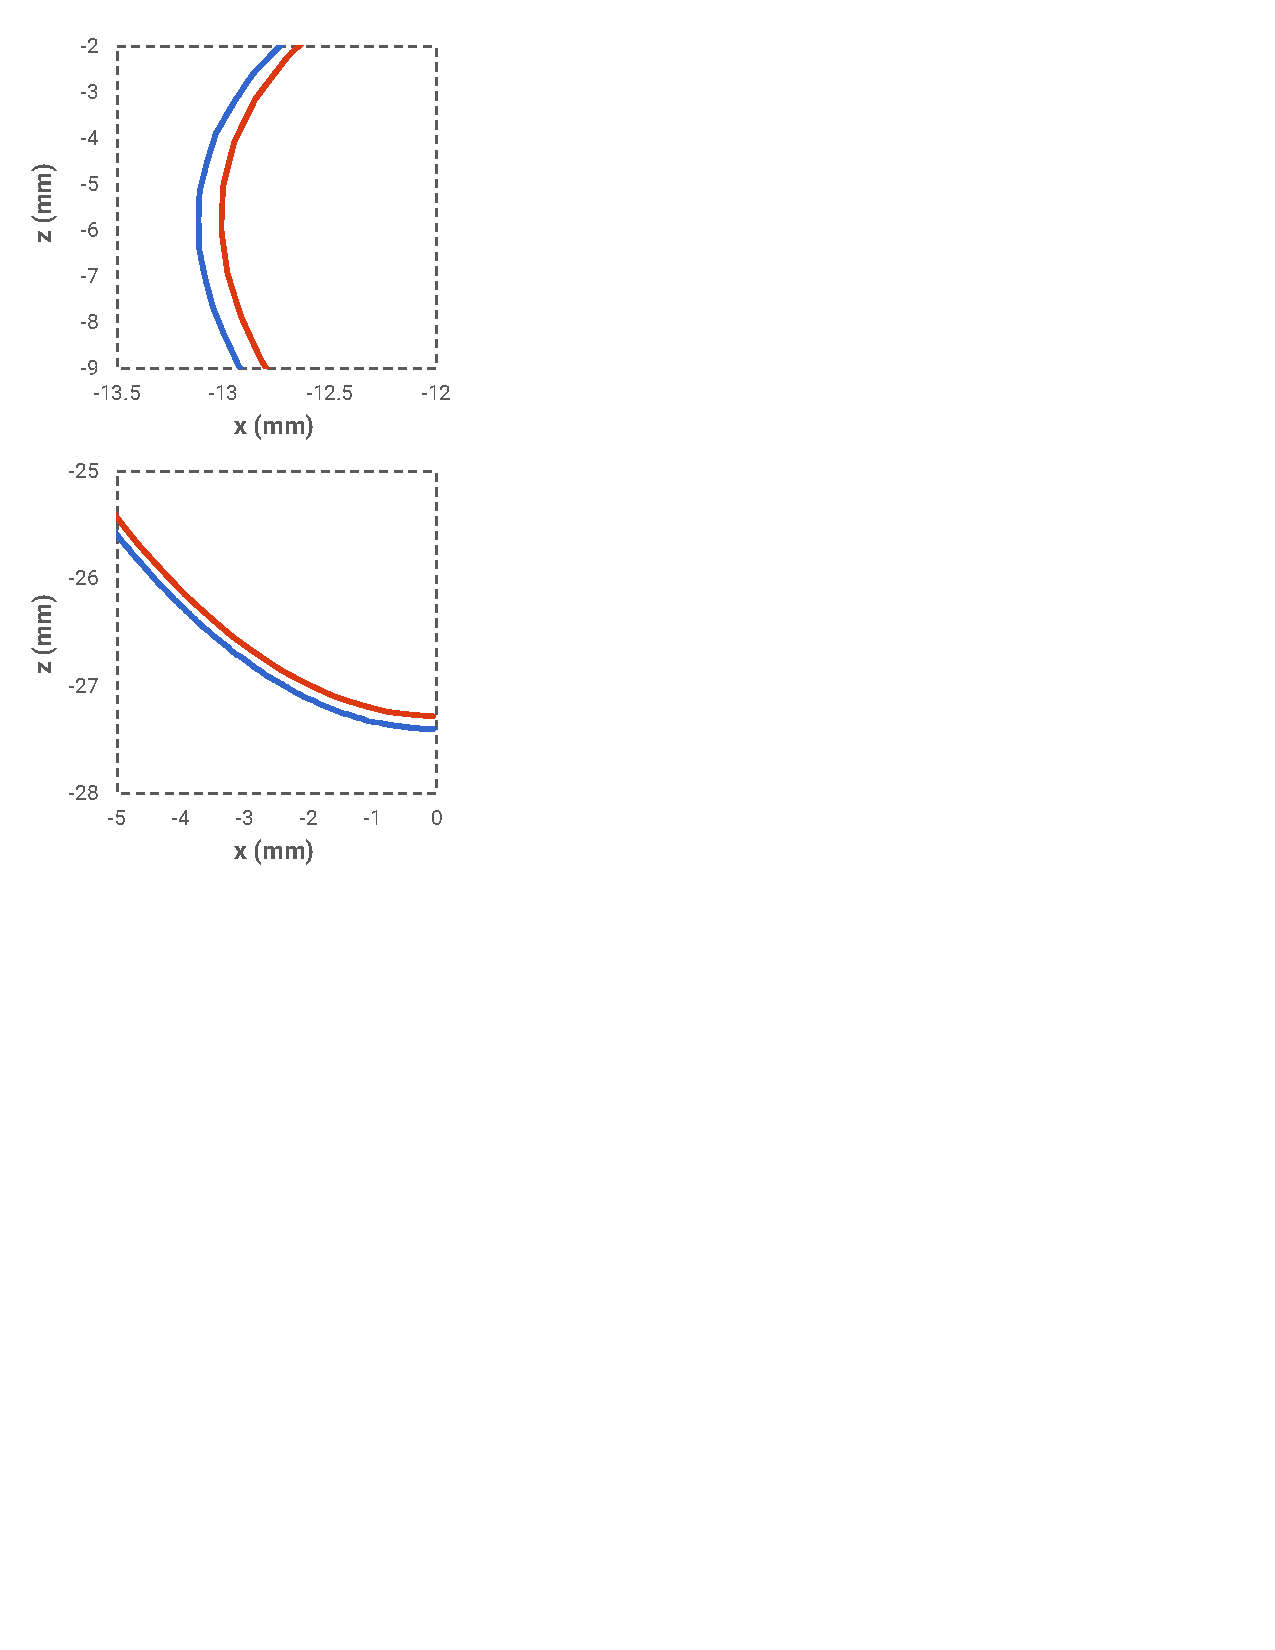
\includegraphics[scale=0.46]{media/5-verif/5-land2/land2-2.pdf}
\label{fig:land2-2}}	
\subfigure[]{%
		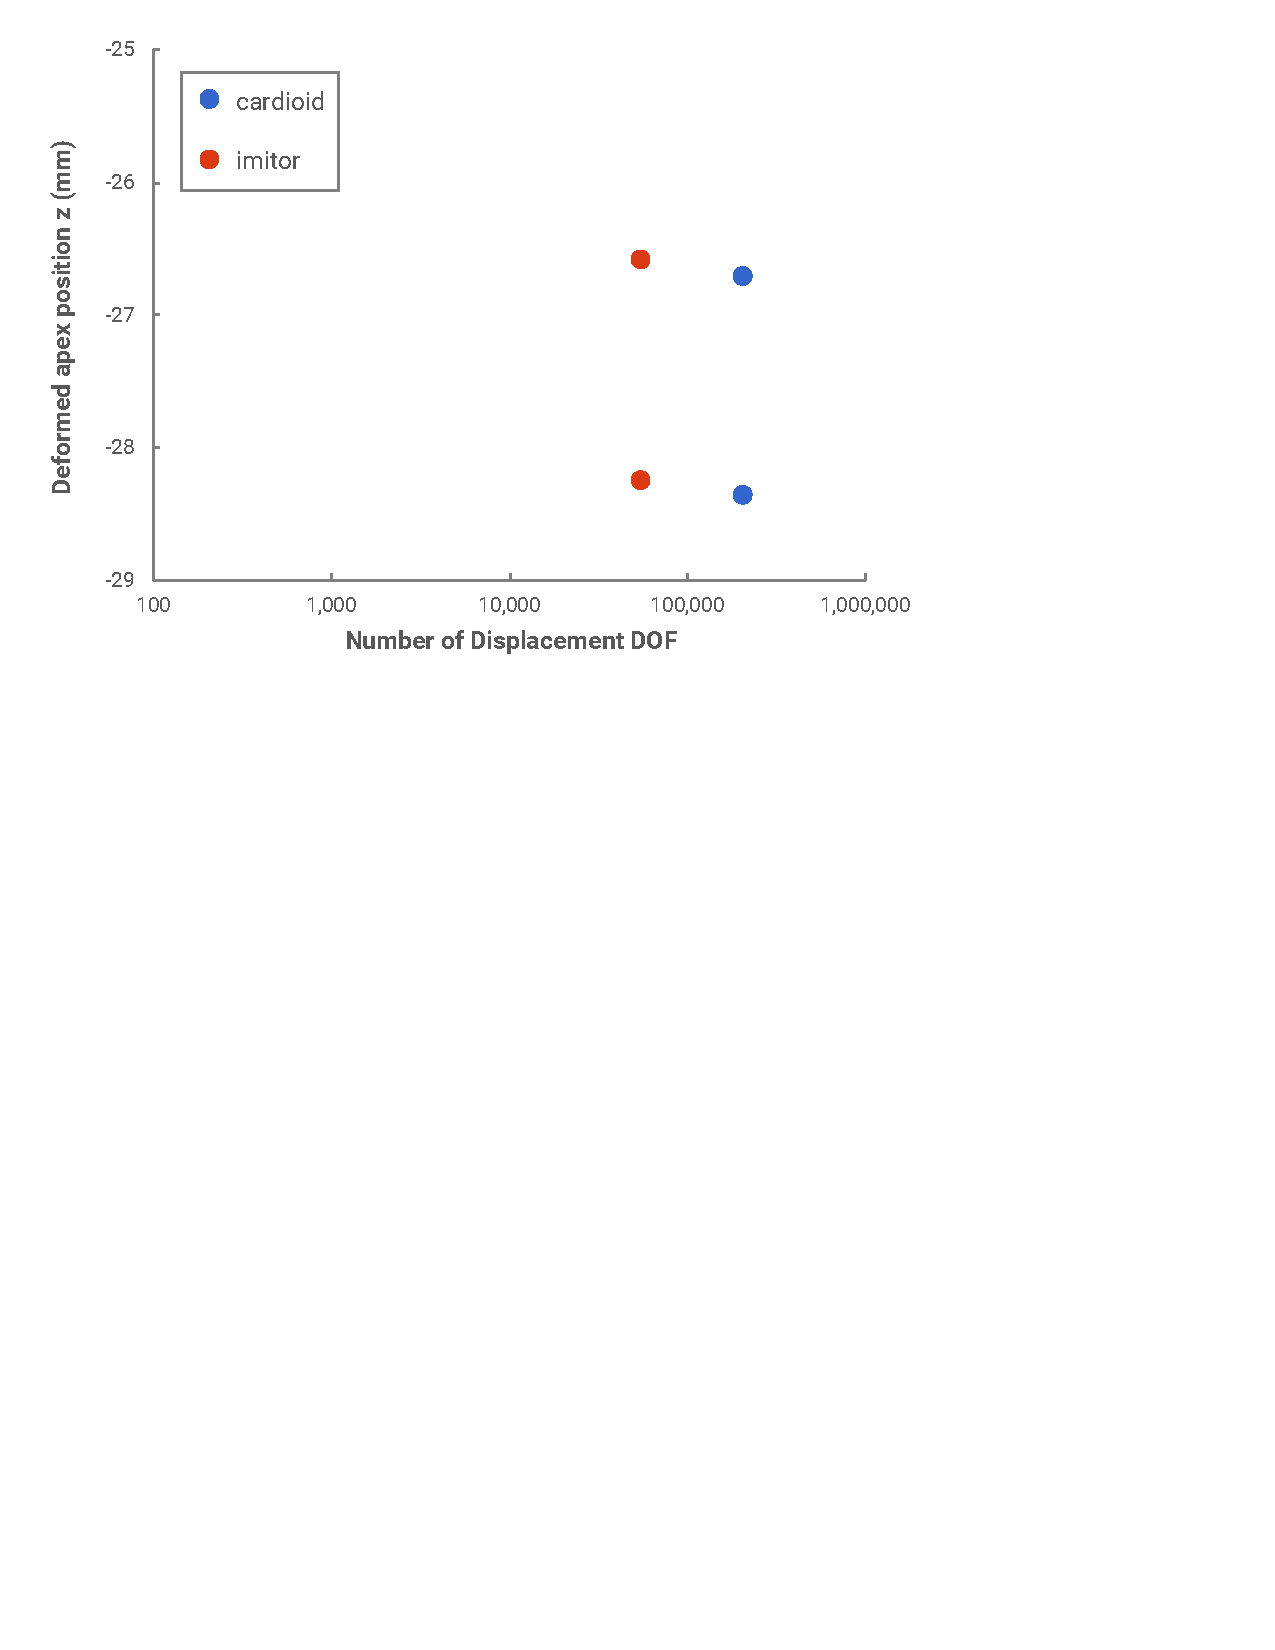
\includegraphics[scale=0.46]{media/5-verif/5-land2/land2-3.pdf}
\label{fig:land2-3}}			
%
\caption{Results for Land P2 verification problem: (a) Deformed position of middle of the ventricle wall, with (b) details at the inflection point (top right) and the apical region (bottom right). Panel (c) shows the deformed position of the apex at the endo- and epicardium for each of the simulation codes.}
\label{fig:land2}
\end{figure}

\begin{figure}[ht!]
\centering
\subfigure[]{%
		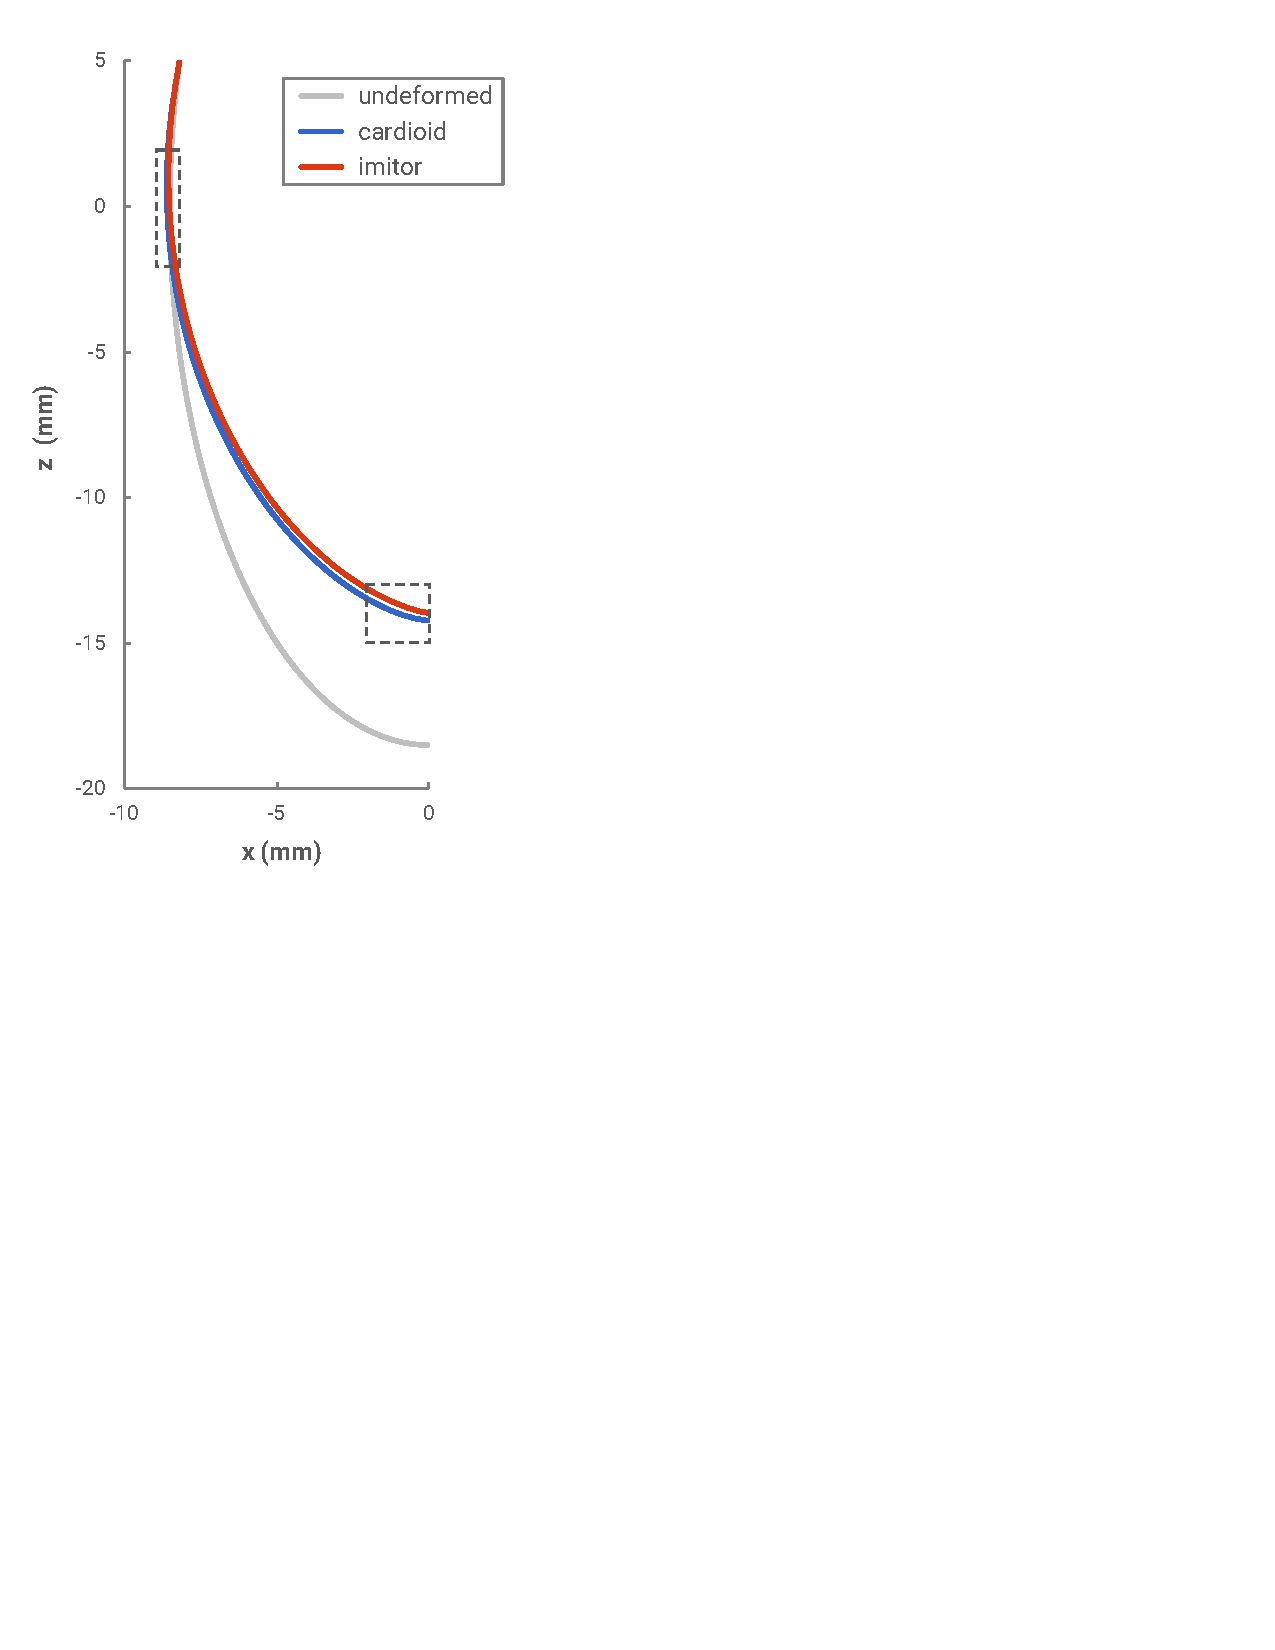
\includegraphics[scale=0.46]{media/5-verif/6-land3/land3-1.pdf}
\label{fig:land3-1}}		
\subfigure[]{%
		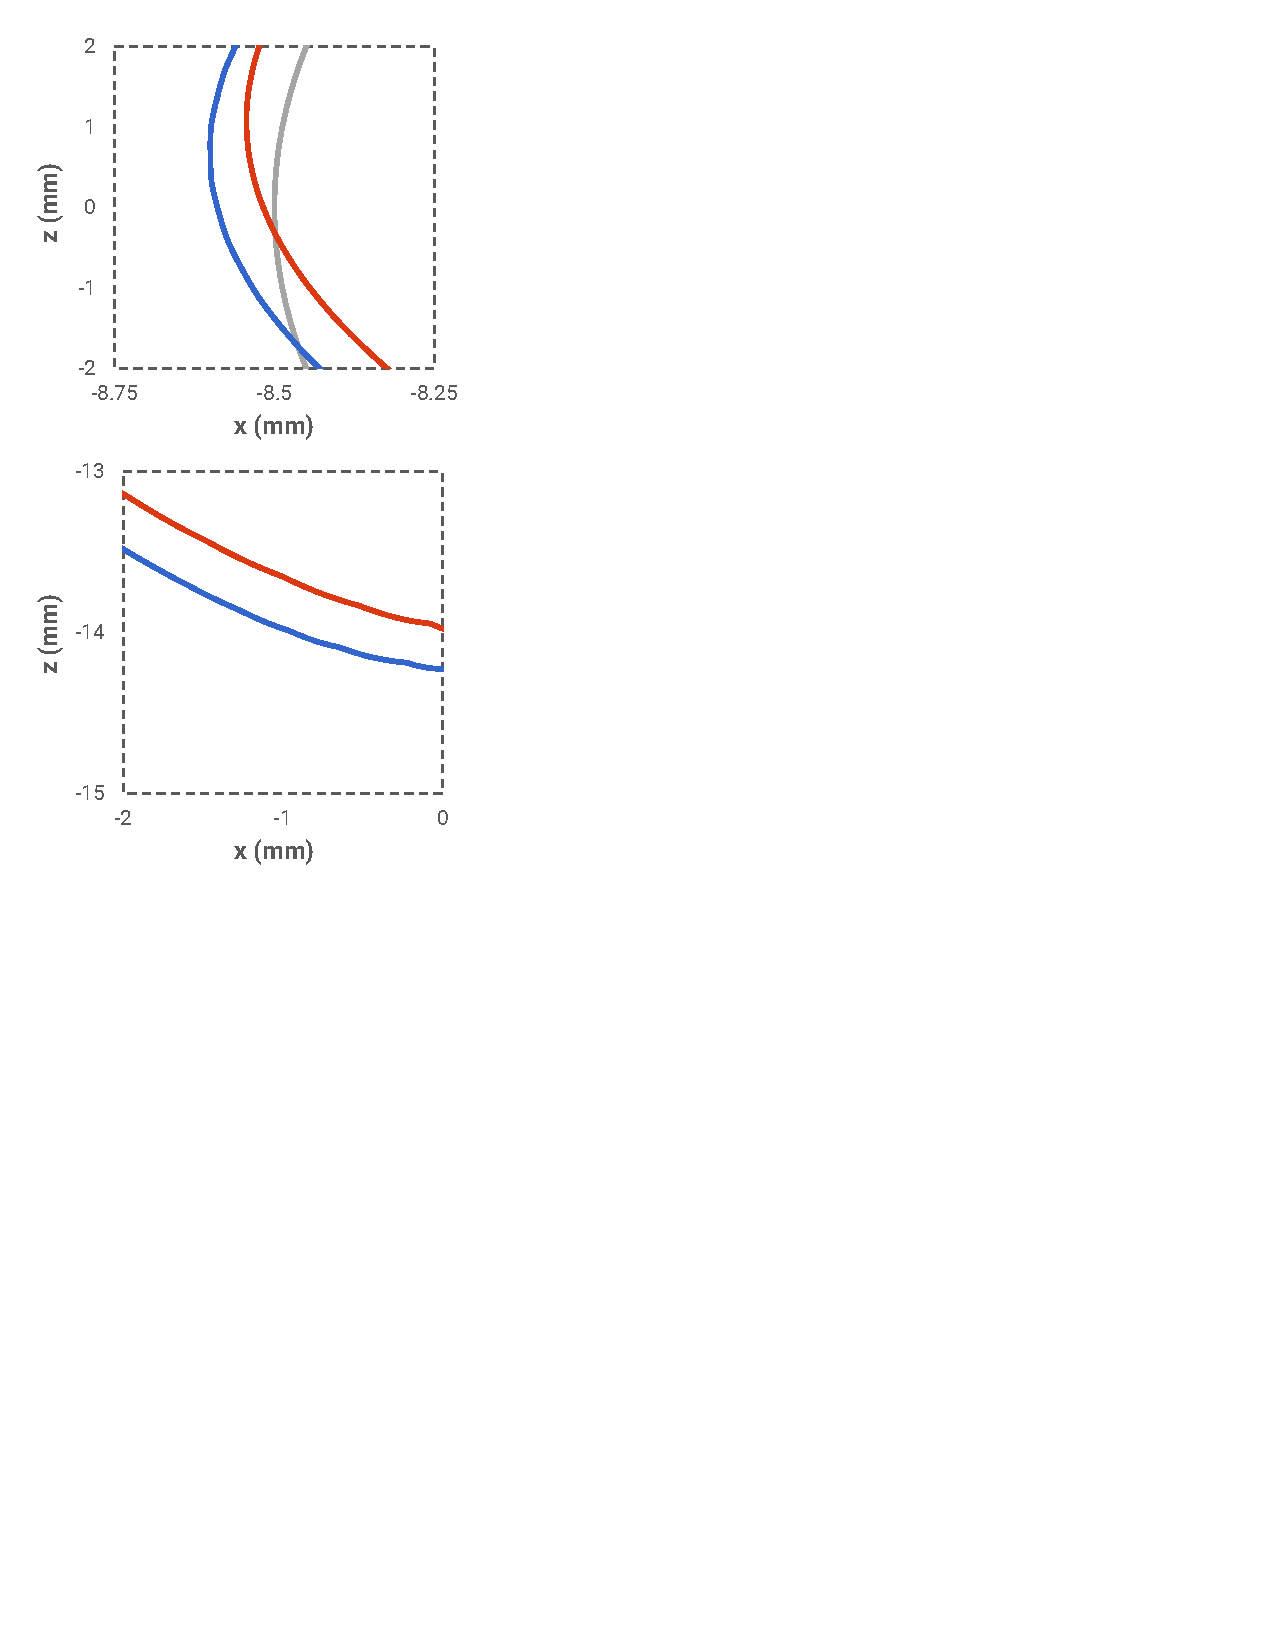
\includegraphics[scale=0.46]{media/5-verif/6-land3/land3-2.pdf}
\label{fig:land3-2}}	
%
\caption{Results for Land P3 verification problem: (a) Deformed position of middle of the ventricle wall, with (b) details at the inflection point (top right) and the apical region (bottom right).}
\label{fig:land3}
\end{figure}

\begin{figure}[ht!]
\centering
\subfigure[]{%
		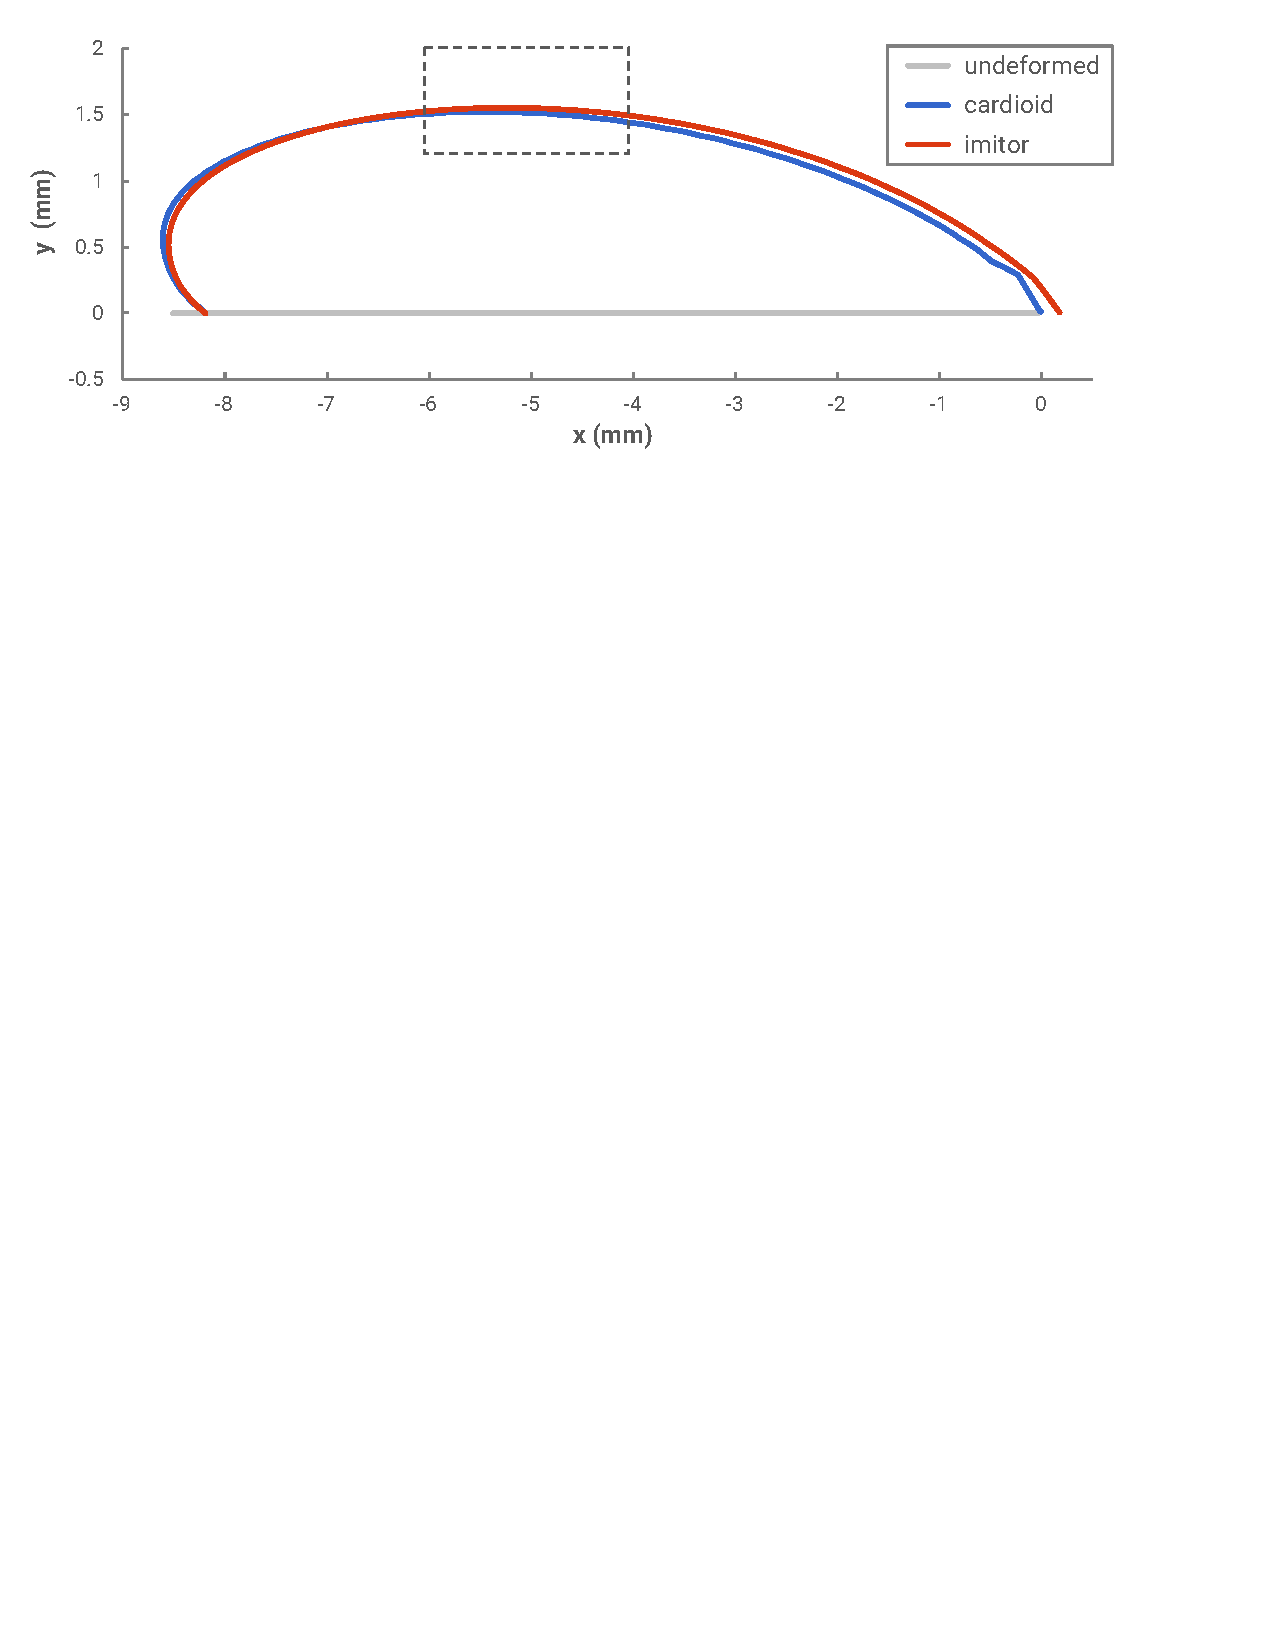
\includegraphics[scale=0.46]{media/5-verif/6-land3/land3-3.pdf}
\label{fig:land3.2-1}}		
\subfigure[]{%
		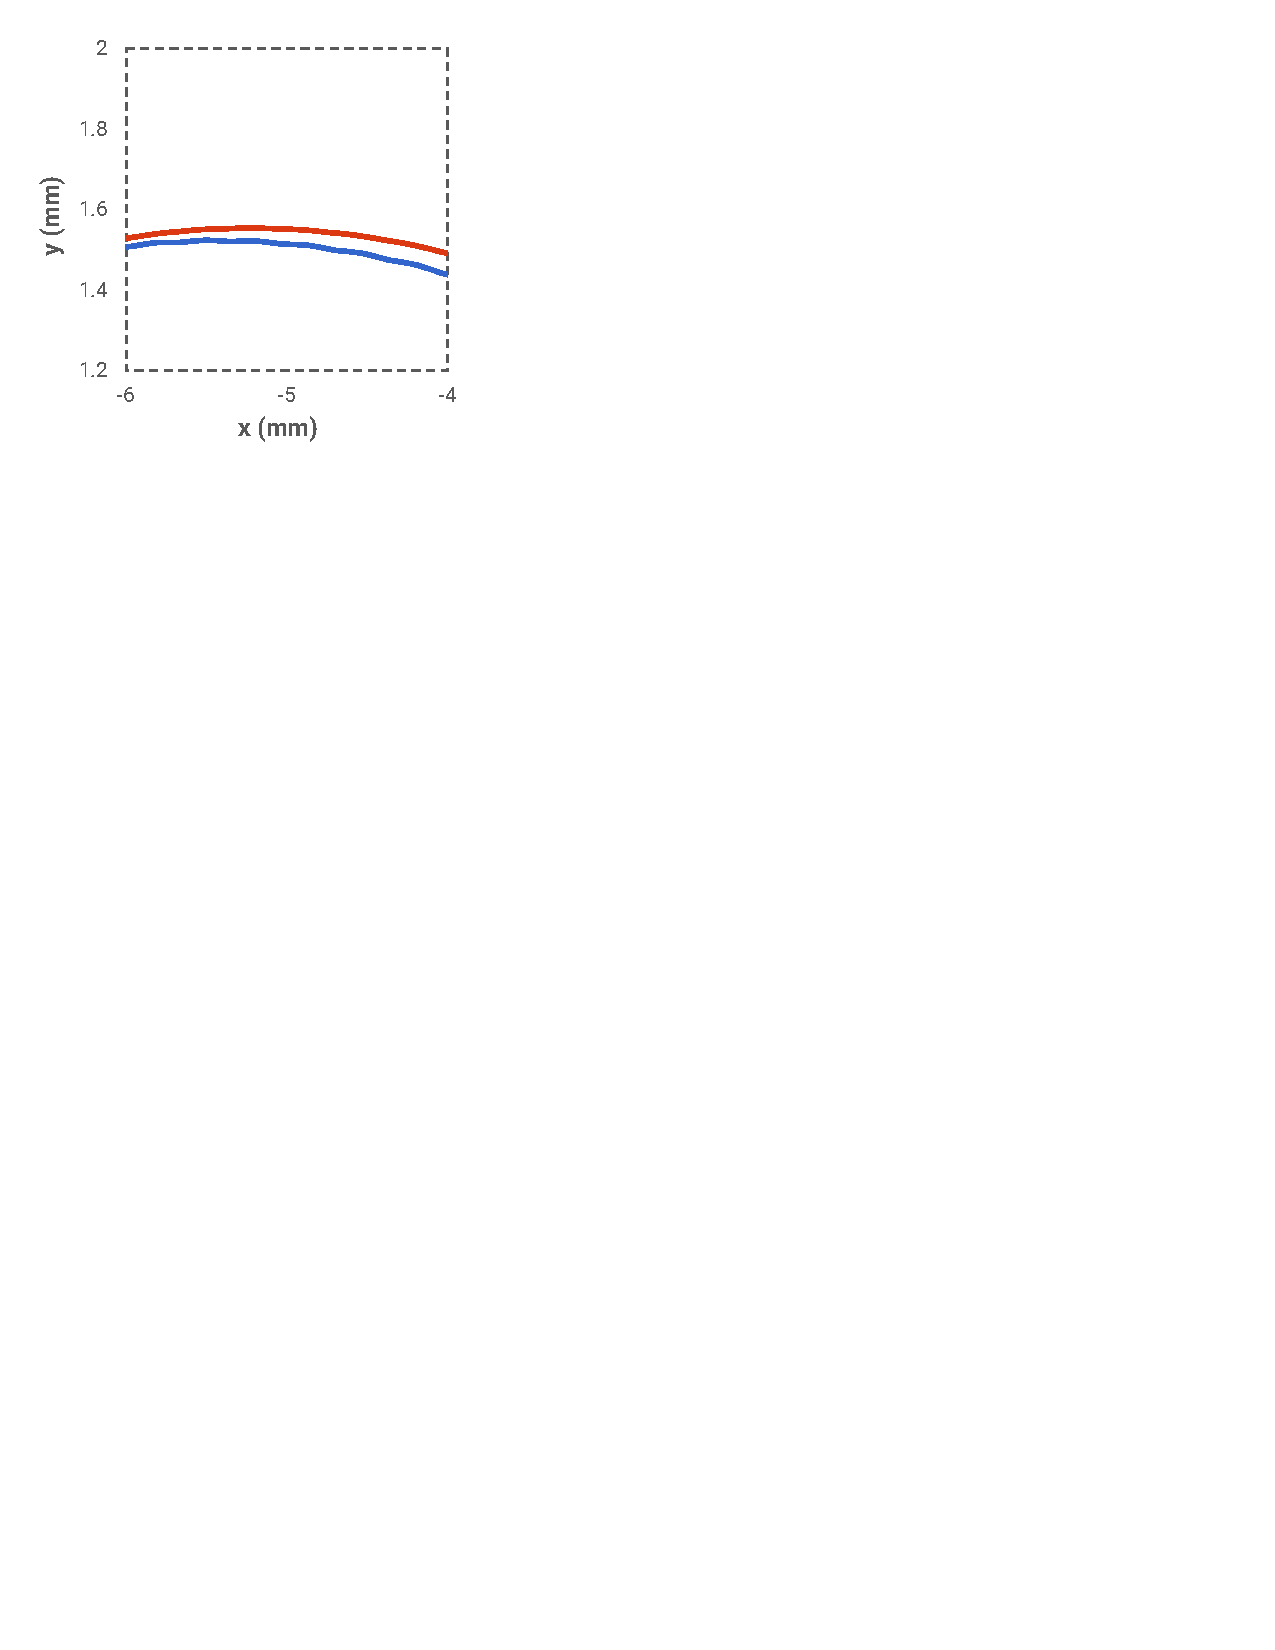
\includegraphics[scale=0.46]{media/5-verif/6-land3/land3-4.pdf}		
\label{fig:land3.2-2}}	
\subfigure[]{%
		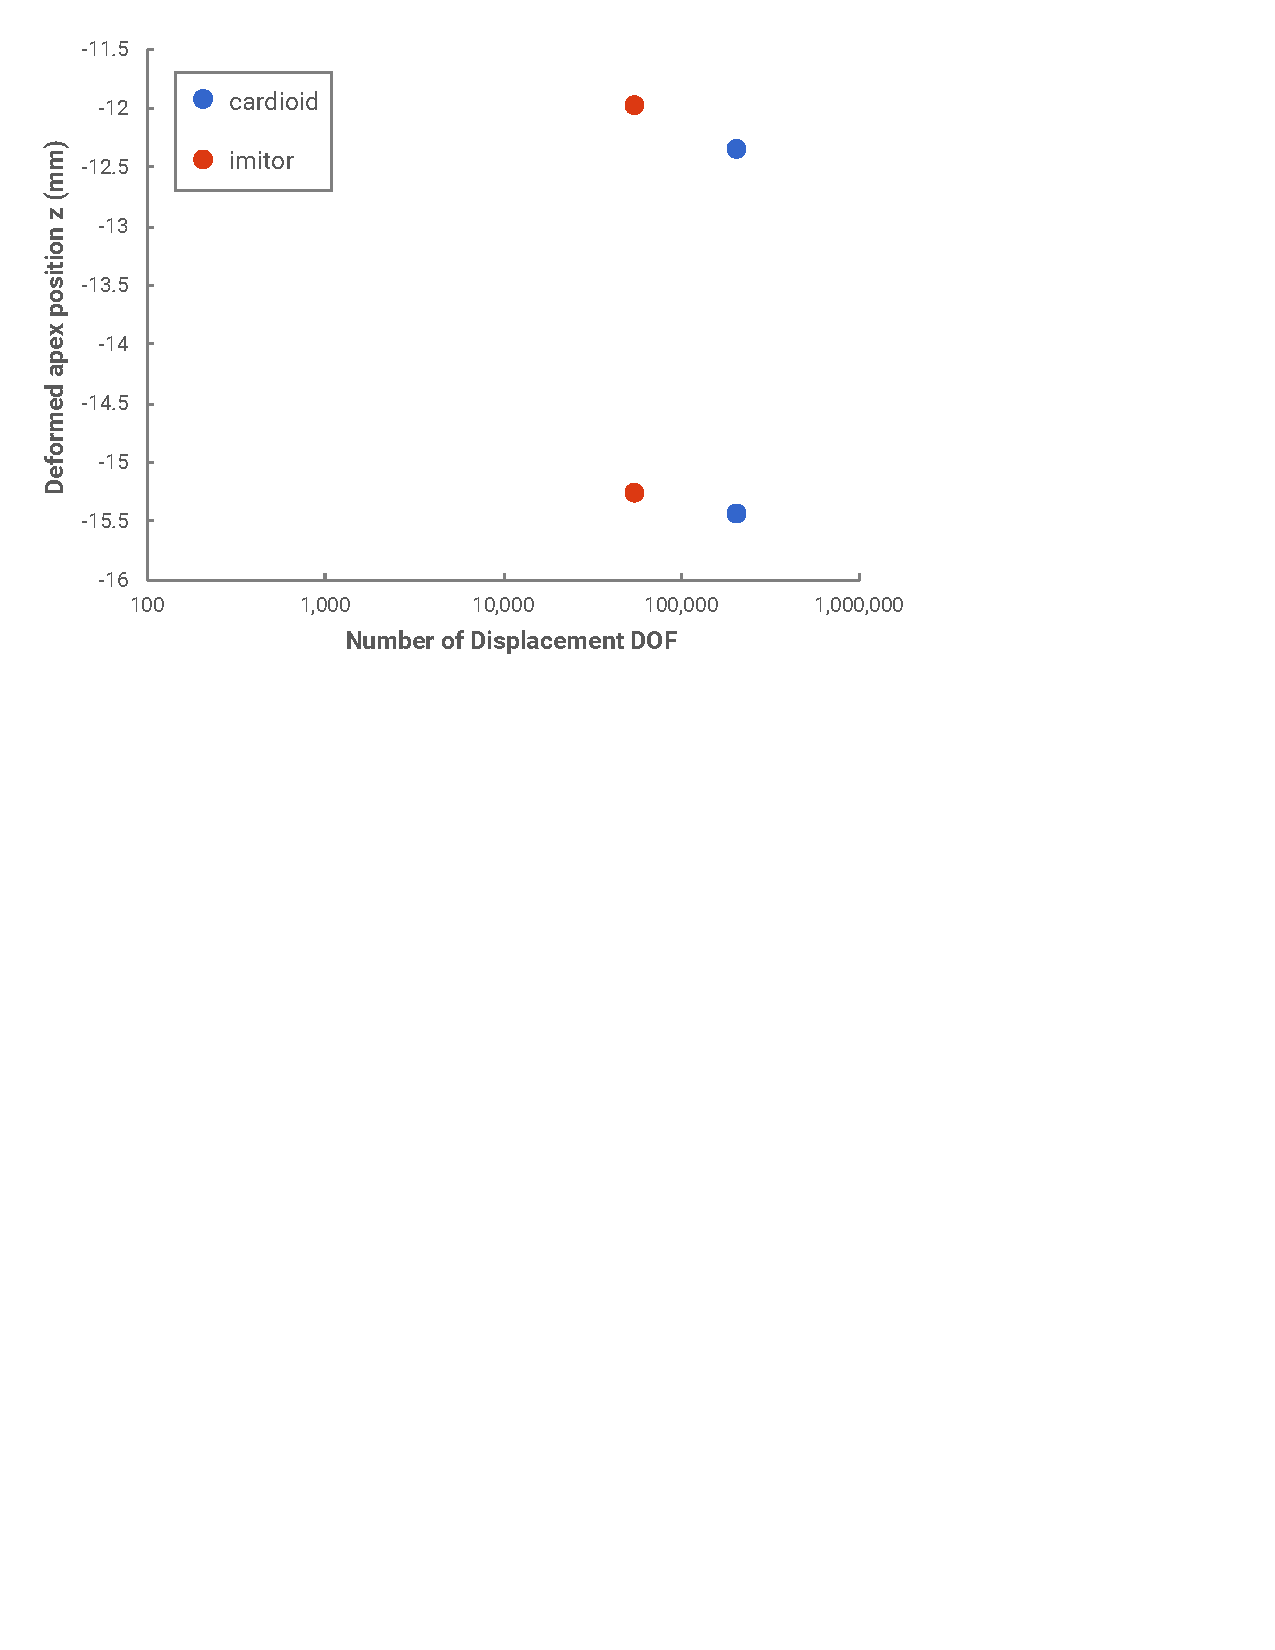
\includegraphics[scale=0.46]{media/5-verif/6-land3/land3-5.pdf}
\label{fig:land3.2-3}}			
	
%
\caption{Results for Land P3 verification problem: (a) The same deformed position of middle of the ventricle wall, shown in the $x-y$ plane, with (b) details at the inflection point. Panel (c) shows the deformed position of the apex at the endo- and epicardium for each of the simulation codes.}
\label{fig:land3.2}
\end{figure}
